\newpage\begin{center}
\parindent=0pt

{\Large Maïeul ROUQUETTE}
\vspace{0.5ex}

{\footnotesize \emph{Avec la participation de}}

\vspace{0.5ex}

{Brendan CHABANNES et Enimie ROUQUETTE}

\vspace{8ex}
{\LARGE\logo~appliqué aux sciences humaines}

\vspace{10ex}
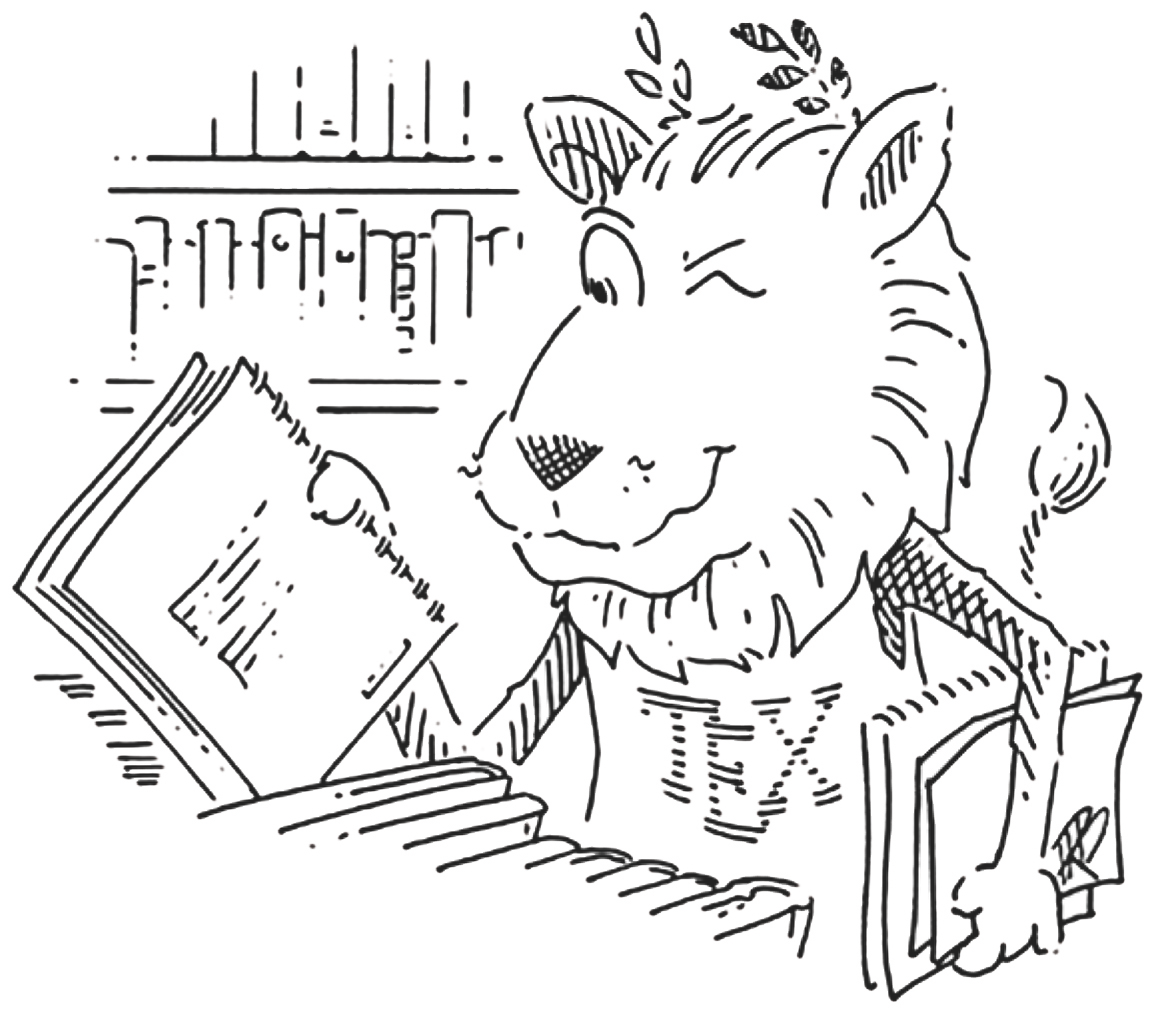
\includegraphics[width=0.75\textwidth]{images/lion.png}
\vspace{3ex}

{\large \emph{Le seul livre sur \LaTeX sans une seule équation !}}

\vspace{28ex}



{\small Publié sous licence \href{http://creativecommons.org/licenses/by-sa/3.0/fr/}{Creative Commons France 3.0 - Paternité - Partage à l'Identique}}
\end{center}
\newpage

\def\epi{Du \LaTeX sed \TeX}
\def\episource{Proverbe Latin}

\phantomsection\part*{Avant-propos\addcontentsline{toc}{part}{Avant-propos}}
\pdfbookmark[0]{Remerciements et détails techniques}{}
\phantomsection\addcontentsline{toc}{section}{Remerciement}\section*{Remerciement}

Nombreuses sont les personnes à remercier pour leurs participations à ce projet. Tout d'abord Brendan Chabannes et ma sœur Enimie qui ont accepté d'écrire plusieurs passages ainsi que Laura Pigeon pour avoir mis en page la première et la quatrième de couverture.

Christophe Masutti m'a incité à écrire ce livre et je ne me serais pas lancé dans cette rédaction sans ses encouragements. Ma reconnaissance va également à mon directeur de mémoire, Rémi Gounelle, qui a aimablement accepté de prendre sur son temps décanal pour discuter de ce projet.

Deux amis astronomes sont également à mentionner : Benjamin pour m'avoir fait découvrir  \LaTeX et Yannick pour m'avoir convaincu, sans le savoir, de l'utiliser pour mon mémoire, au cours de l'une de nos nombreuses conversations électroniques.

Je tiens également à remercier l'ensemble de la communauté \LaTeX sans qui ce livre n'aurait pu exister, faute d'objet. 


\newpage
\phantomsection\addcontentsline{toc}{section}{Au sujet de ce livre}\section*{Au sujet de ce livre}\thispagestyle{plain}

Il va de soi que ce livre a été composé avec \XeLaTeX. Outre les packages dont il traite, j'ai utilisé les packages  \package{minted} pour les citations de code ; ainsi que \package{mdframed} et \package{framed} pour les boîtes colorées.



Ce livre est diffusé sous licence \emph{Creatives Commons - Paternité - Partage des Conditions Initiales à l'Identique 3.0 France}. Sommairement\footnote{Pour les détails, je renvoie au texte intégral de la licence : \url{http://creativecommons.org/licenses/by-sa/3.0/fr/legalcode}.}, cela signifie que vous pouvez le diffuser, le dupliquer, le publier et même le modifier si vous respectez deux conditions:
\begin{enumerate}
\item que vous citiez mon nom\footnote{Et que vous ne portiez  pas atteinte à mes droits moraux.};
\item que vous offriez les mêmes droits aux destinataires de vos diffusions\footnote{Les images de pas et d'éclair servant à indiquer les encarts sont tirées du domaine public et (légèrement) modifiées par mes soins. Elles ne sont donc pas affectées par ces règles. Voir \url{http://www.openclipart.org/detail/154855/green-steps-by-netalloy} et \url{http://thenounproject.com/noun/high-voltage/}. L'image de couverture est de Duane  Bibby, avec une légère modification. Voir \url{http://www.ctan.org/lion.html}.}.
\end{enumerate}

Bien sûr, si vous souhaitez me soutenir, vous pouvez acheter cet ouvrage en version papier, ou simplement m'envoyer un petit mot (vous trouverez aisément comment me contacter sur Internet).

Si vous souhaitez améliorer cette œuvre, soyez le bienvenu. Le code est mis à disposition sur GitHub\footnote{À l'adresse \url{https://github.com/maieul/latexhumain}.}, un service fonctionnant à l'aide de l'outil de travail collaboratif Git\renvoi{svn} mais disposant d'une interface d'édition en ligne. 

N'hésitez pas à me demander un accès à l'édition du projet ! 


\chapter{\LaTeX{} : définition et intérêts}

\begin{prealable}
 Dans ce chapitre nous allons vous présenter brièvement \LaTeX{} et les raisons pour lesquelles nous pensons que son apprentissage est utile pour la rédaction de travaux en sciences humaines.
\end{prealable}

\section{Pourquoi \LaTeX{} ?}

\subsection{Inconvénient des traitements de textes}

Quand vous rédigez un texte dans votre traitement de texte, comme par exemple Microsoft Word ou Openoffice.org, celui-ci exécute deux actions simultanées :

\begin{itemize}
\item D'une part il stocke dans un fichier la structure logique de votre texte : titres, paragraphes, notes de bas de pages etc.
\item D'autre part il vous affiche à l'écran le rendu \enquote{physique} de votre texte (justifications, gras, italiques etc), tel qu'un lecteur en disposera.
\end{itemize}

Pour cette raison on appelle ce type de logiciel WYSIWYG, ce qui en anglais signifie \textenglish{What You See Is What You Get}\footnote{\enquote{Ce que vous voyez est ce que vous faites}.}. 

Cette combinaison de deux fonctions différentes dans les  traitements de texte a trois conséquences :

\begin{itemize}
\item La nécessité d'afficher en temps réel le rendu physique du texte tout en conservant une vitesse relativement élevée du logiciel entraîne une baisse de la qualité typographique. Par exemple :
	\begin{itemize}
		\item Pour avoir un texte justifié à gauche et à droite, les traitements de texte font varier la taille des espaces entre les mots. Les variations peuvent parfois être considérables ce qui peut diminuer le confort de lecture. Pour éviter ce type d'ennui, les livres \enquote{classiques} coupent les mots en fin de ligne, ce qu'on appelle une césure\footnote{La césure ne se fait toutefois pas n'importe où : elle doit respecter des règles propres à chaque langue.}.
		\item Les blancs situés avant certains signes de ponctuations, comme par exemple les points d'exclamation font la même taille que les blancs séparant les mots, alors que les règles typographiques \enquote{classiques} prévoient des blancs plus petits.
	\end{itemize}
\item Le fait qu'un même logiciel s'occupe \emph{à la fois} de l'affichage et de la structure du texte incite à confondre les deux. Ce qui peut avoir deux effets négatifs, qui ne sont pas systématiques toutefois\footcite[Les auteurs de ces lignes sont moins sévères envers les traitements de texte que d'autres LaTeXiens : \cf][]{stupide}:
	\begin{itemize}
		\item Cela peut inciter à se concentrer sur le forme plutôt que sur le fond et la structure. Toutefois en théorie la formation universitaire de sciences humaines incite à penser \emph{structure et sens d'abord}\footcite[Voir un débat sur le blog d'un des auteurs]{structurevsforme}. 
		\item Les rédacteurs n'utilisent pas toujours la possibilité de séparer sens et forme grâce aux styles. Dans ces cas, lorsqu'on désire changer la forme d'un élément logique (par exemple le titre d'un chapitre) on doit changer l'ensemble des endroits où cet élément logique est utilisé\footnote{Par exemple, pour une personne  qui n'aurait pas utilisé les styles pour désigner ses titres de chapitre, il faudra sélectionner \emph{l'ensemble des titres de chapitres} puis aller dans les menus de mise en forme etc.}.
	\end{itemize}

\item Les lourds calculs informatiques nécessaire au calcul de la mise en forme en temps réel rendent les traitements de textes particulièrement lents comparativement à d'autres logiciels. Cette lenteur est souvent source d'énervement et de pertes de concentration. Pour compenser, ces logiciels exigent bien souvent du matériel récent.
\end{itemize}

En outre, si les traitements de textes récents disposent d'outils de gestions de bibliographies, ceux-ci manquent en général de souplesse, c'est pourquoi ils sont rarement utilisés. Ainsi nombreux sont les auteurs à écrire directement leur bibliographie \enquote{à la main} en tapant directement : Nom de l'Auteur, \emph{Titre}, etc. En cas d'erreur ils faut donc corriger l'ensemble des endroits où l'œuvre est citée.

\subsection{Avantage de \LaTeX{}}

\LaTeX{} permet de résoudre l'ensemble des problèmes des traitements de texte. En effet, \LaTeX{} sépare deux étapes : 

\begin{itemize}
\item L'étape de rédaction, qui se passe dans un éditeur de texte. L'auteur frappe son texte et indique par un certain nombre de commandes sa structure (titres, paragraphes, notes de bas de pages).
\item L'étape de calcul de l'affichage se fait seulement ensuite : l'auteur fait passer son fichier par un \concept{compositeur}, parfois aussi appelé \concept{compilateur}\footnote{Qu'on peut sommairement décrire comme un ensemble de scripts informatiques.}. Ce dernier programme va lire l'ensemble des commandes du fichier pour produire un nouveau fichier au format \ext{.pdf}\footnote{Historiquement \LaTeX{} produisait un autre format de fichier : \ext{dvi}. Mais pour notre propos, cela n'a pas d'importance : dans ce livre nous n'utiliserons que la production de \ext{pdf}.}.
\end{itemize}

Cette séparation permet :
\begin{itemize}
\item Une qualité typographique supérieure :  le compositeur n'étant pas contraint par la nécessité d'un affichage en temps réels, il peut faire des calculs plus lourds : ainsi par exemple \LaTeX{} produit des césures typographiques et non pas des blancs à géométrie variable, et équilibre bien mieux la composition du texte.
\item Une meilleure séparation du sens et de la forme\footnote{Qui répétons-le est toutefois possible avec les logiciels WYSIWYG.} puisque l'auteur donne uniquement des indications de sens.
\end{itemize}

En outre \LaTeX{} possède un système de gestion de la bibliographie extrêmement puissant. Il permet à l'auteur de séparer le contenu de sa bibliographie\footnote{Titres, auteurs etc.} de son affichage\footnote{Faut-il mettre des \emph{op. cit.}, et si oui où ; faut-il mettre uniquement les initiales des prénoms ou les prénoms en entier etc.}.

Cette séparation entre contenu de la bibliographie et affichage est utile non seulement aux auteurs mais aussi aux éditeurs. En effet, si l'auteur structure correctement sa base de donnée bibliographique\renvoi{bddbiblio} l'éditeur peut adapter l'affichage de la bibliographie à ses propres règles : il lui suffit de créer des fichiers de styles bibliographiques, suivant une syntaxe simple.

La gestion d'une bibliographie est à la fois l'un des travaux les plus importants en sciences humaines \emph{et} l'un des plus pénibles, avec des nombreuses sources d'erreurs possibles. Cette simple raison suffit aux yeux des auteurs à préférer \LaTeX{} à un logiciel de traitement de texte\footnote{Les deux auteurs se sont décidés à utiliser \LaTeX{} dans le cadre de leurs travaux universitaires, et l'élément déclencheur du choix a été la facilité et la souplesse de la gestion bibliographique.}.

\subsection{Qu'est qu'un éditeur de texte ?}

Nous avons parler dans ces paragraphes de deux types de logiciels, qu'il ne faut pas confondre :
\begin{itemize}
	\item Les traitements de texte.
	\item Les éditeurs de texte.
\end{itemize}

Nous avons vu ce qu'était les premiers : des logiciels qui s'occupent d'insérer dans un fichier la structure logique d'un texte \emph{et} de montrer son rendu physique.
Les seconds sont simplement des logiciels qui permettent à une personne d'écrire dans un fichier texte et de placer lui même ses commandes de structurations.
Toutefois les bon éditeurs de texte font plus que permettre d'écrire dans un fichier texte : ils aident à sa rédaction par différents outils :
\begin{itemize}
\item Souvent ils colorient à l'écran les commandes, afin de permettre de mieux les visualiser; c'est ce que l'on appelle la coloration syntaxique.
\item Ils proposent des raccourcis pour taper les commandes les plus fréquentes :  raccourcis clavier, boutons etc.
\item Ils proposent parfois un affichage du plan du travail.
\end{itemize}

Certains de ces éditeurs de texte sont généralistes et adaptés à plusieurs langages informatiques\footnote{Par exemple le \LaTeX{} et le HTML, ce dernier étant utilisé pour les sites internet}. D'autres sont spécialisés dans tel ou tel langage : ils proposent en général des outils supplémentaires propres au langage de spécialisation. 

Par exemple les éditeurs spécialisés en \LaTeX{} proposent des boutons spécifiques afin de lancer le compositeur \LaTeX{}.

Pour commencer en \LaTeX{} il vous faudra donc abandonner votre ancien traitement de texte et choisir un éditeur de texte spécialisé en \LaTeX{} : nous en listons plusieurs en annexes\renvoi{annexe:editeurs}.

\section[TeX, LaTeX, XeTeX, XeLaTeX : points communs et différences]{\TeX{}, \LaTeX{}, \XeTeX{} et \XeLaTeX{} : points communs et différences}

Dans ce chapitre nous avons parlé de \LaTeX{}. Le titre de ce livre parle pourtant  de \XeLaTeX{}. Quelle est la différence ? Voici une brève explication historique, très simplifiée\footnote{Le lecteurs curieux trouvera aisément de la documentation plus détaillée sur le sujet.}.

\begin{enumerate}
\item En 1977 Donal Knuth invente  \TeX{} qui était un simple compositeur de texte, capable de transformer un texte structuré par des commandes en un texte mis en forme. Avec \TeX{} on pouvait également inventer ses propres commandes.
\item L'utilisation de \TeX{} était relativement complexe. Pour simplifier cela Leslie Lamport a créé un ensemble de commandes \TeX{}. Cet ensemble de commande a permis de former le langage \LaTeX{} et le compositeur associé.
\item Par la suite un compositeur dérivé de \TeX{} a été créé : \XeTeX{}. Ce compositeur permet deux choses :
\begin{itemize}
	\item Une gestion native de l'ensemble des écritures mondiales, par le biais du jeu de caractères Unicode\renvoi{utf8}.
	\item Une gestion native des nouvelles polices de caractères au format OpenType\footnote{Ce type de fonte permet une gestion poussée des ligatures entre les caractères, par exemple. Le lecteur curieux trouvera aisément de la documentation techniques sur le sujet.}, apparus au début des années 2000.

\end{itemize} 
\item Pour permettre d'utiliser les commandes de \LaTeX{} avec \TeX{} on a créé \XeLaTeX{}.
\end{enumerate}

On peut résumer les liens entre \TeX{}, \LaTeX{}, \XeTeX{} et \XeLaTeX{} par le schéma \ref{sch:tex} (p. \pageref{sch:tex}).

\begin{figure}[ht]
\centering
% Schéma des parentes entres TeX LaTeX XeTeX etc.
\begin{tikzpicture}
	
	% Les textes
	\node[text height=1ex,anchor=mid] (T) at (0,0) 		 	{\TeX} ;
	\node[text height=1ex,anchor=mid]  (X) at (1, -2)	 	 	{\XeTeX};
	\node[text height=1ex,anchor=mid]  (L) at (-1, -2) 		{\LaTeX};
	\node[text height=1ex,anchor=mid]  (XL) at (0,-4)			{\XeLaTeX};
	
	% Les traits
	\draw[->] (T) -- (X.north);
	\draw[->] (T) -- (L.north);
	\draw[->] (L) -- (XL.100);
	\draw[->] (X) -- (XL.80);
\end{tikzpicture}

\caption{Les relations entre \TeX{}, \LaTeX{}, \XeTeX{} et \XeLaTeX{}}\label{sch:tex}
\end{figure} 

Dans  ce livre nous travaillerons sur \XeLaTeX{}. Toutefois comme la plupart de nos propos peuvent s'appliquer indifféremment  à \LaTeX{} et à \XeLaTeX{}, nous parlerons de \LaTeX{}, sauf lorsque nous signalerons une spécificité de \XeLaTeX{}.

\begin{anedocte}
Bien que le sujet soit controversé, il semblerait qu'il faille prononcer le  \forme{X} de \TeX{} comme un \forme{χ} grec\footnote{\forme{Latek}}, car le nom \TeX{} viendrait du mot grec \forme{\textgreek{τέχνη}} : \forme{art, sciences}.
\end{anedocte}



\def\epi{Les Sabins \textelp{} commencerent la bataille, qui fut aspre \& dura longuement}
\def\episource{\cite{Sabins}}

\part{Premiers pas avec \LaTeX}
\chapter[Commencer avec XeLaTeX]{Commencer avec \XeLaTeX}\label{commencer}

\begin{prealable}
Nous supposons que vous avez installé \LaTeX et un éditeur de texte spécialisé en \LaTeX. Voyez en annexe. \renvoi{install}\renvoi{logiciel}

La première chose à faire est de vérifier que ce logiciel de traitement de texte enregistre bien en UTF-8\footnote{Le réglage se trouve en général dans les préférences du logiciel, dans une rubrique \emph{enregistrement} ou \emph{encodage} : consultez le manuel de votre logiciel le cas échéant.}. Nous reviendrons plus loin\renvoi{utf8} sur l'intérêt d'un tel encodage, sachez simplement que il permet d'utiliser des signes non latins\footnote{Cyrilliques, grecs, sanskrits, hébraïques etc. Et même extra-terrestres.}.

\end{prealable}

\section{Un premier document}

Dans votre éditeur de texte, frappez le code suivant :\footnote{Comme nous l'avons expliqué en introduction (p.~\pageref{colorationsyntax}), la coloration que vous voyiez ici, si vous lisez la version informatique de ce livre, a un sens syntaxique : ne vous préoccupez pas de savoir comment cela apparaîtra dans votre éditeur, et ne pensez pas que cela apparaîtra ainsi une fois compilé.} puis cliquez sur le bouton de compilation avec \XeLaTeX \footnote{Sa position dépend de votre éditeur de texte. Pour le moment vous pouvez vous contenter de ce bouton, mais un jour vous devrez apprendre à faire quelques lignes de commandes : ne vous inquiétez pas, tout sera expliqué.} :

\inputminted{exemples/premierpas/notions/1.tex}


Regardez le PDF obtenu :  afin de comprendre les principes de base de \LaTeX nous allons lire le code que vous avez copié et le commenter ligne par ligne.

\section{Structure d'un document \LaTeX}

\subsection{La classe du document}
La première ligne \csp{documentclass}\verb|[12pt]{book}| déclare la classe du document, ici \classe{book}. Une classe correspond à un choix éditorial    --- mise en page et organisation générale du document. Le choix de la classe influence entre autre :
\begin{itemize}
\item Le nombre de niveaux de titre disponibles.
\item Les marges appliquées.
\item Les en-têtes et pieds de page.
\end{itemize}

Il existe en standard plusieurs classes de documents : citons \classe{book}, pour rédiger un livre ; \classe{article} pour un article (si, si !) ; \classe{beamer} pour un présentation sous forme de diapositive à projeter. Dans cet ouvrage, nous aborderons essentiellement les deux premières, nous ferons également une brève présentation de \classe{beamer}\renvoi{beamer}.



Tout document \LaTeX doit commencer par une déclaration de classe, avant toutes autres lignes. La syntaxe est la suivante : \cs{documentclass}\oarg{options}\marg{classe}

\begin{attention}
Dans la suite de ce livre, tout texte situé entre crochets (\arg{ainsi}), doit être remplacé dans votre fichier \ext{tex} par une valeur textuelle.
\end{attention}

Les options viennent spécifier certaines propriétés de la classe. Dans notre exemple, nous précisons que la taille de la police du texte courant doit être de 12~pt et que le format du papier est A4. Vous pouvez indiquer plusieurs options, en les séparant par des virgules. \label{optionsclasse}. 

Voici quelques options disponibles et utiles en sciences humaines :

\begin{description}
\item[10pt] pour une police de base en 10 pt.
\item[11pt] pour une police de base en 11 pt.
\item[12pt] pour une police de base en 12 pt.
\item[onecolumn] pour un texte sur une seule colonne. C'est le cas par défaut sur les classes citées.
\item[twocolumn] pour un texte sur deux colonne.
\item[oneside] pour une impression en recto seulement. \label{nbsides}
\item[twoside] pour une impression en recto-verso\footnote{Cette option et la précédente servent essentiellement pour les question de reliure. En effet, l'option \option{twoside} produit des marges gauches et droites de tailles différentes, la taille des marges dépendant du caractère recto ou verso de la page. En outre la numérotation des pages est inscrite à gauche et à droite  en alternance.}.\label{rectoverso}
\end{description}

Nous en préciserons d'autres au fur et à mesure de l'ouvrage, lorsque les notions requises auront été abordées.

\subsection{L'appel aux packages}

Voyons les trois lignes suivantes : 
\begin{minted}[linenos,firstnumber=2]{latex}
\usepackage{fontspec}
\usepackage{xunicode}
\usepackage{polyglossia}
\end{minted}

Il s'agit, comme vous auriez pu le deviner, d'appel à des packages\footnote{Nous avons fait volontairement le choix de ne pas traduire ce terme, pour éviter des confusions.}. Un package est un ensemble de fichiers qui ajoutent des fonctionnalités à \LaTeX, c'est l'équivalent d'un plugin sous Firefox. 

Le premier package est \package{fontspec}. Il est utile à \XeLaTeX  pour une typographie avancée, notamment pour disposer d'accents dans le document PDF produit. 

Le second package est \package{xunicode}. Il permet de gérer l'unicode, autrement appelé UTF-8\footnote{En réalité UTF-8 n'est pas tout à fait Unicode, mais une implémentation de ce dernier. Toutefois, pour simplifier, nous assimilons les deux.}. Il nous permet d'utiliser des caractères non-latin dans le document \ext{tex}.\renvoi{utf8}


Le troisième, \package{polyglossia} permet de gérer facilement un document multilingue\renvoi{i18n} et les changements typographiques qu'un tel document implique.

C'est trois packages sont propres à \XeLaTeX  : ils ne fonctionnent pas avec \LaTeX.\ref{TeXLaTeX}

Certains packages peuvent recevoir des options qui modifieront leur comportement standard. La syntaxe est alors \csp{usepackage}\oarg{options}\marg{package}

Tout au long de cet ouvrage, nous aborderons divers packages.

\subsection{Le fran\c cais, langue par défaut\label{french}}

Tout de suite après, la ligne \csp{setmainlanguage}\verb|{french}| indique que nous utilisons comme langue principale du document le fran\c cais\renvoi{i18n}, et donc que le compositeur de texte devra prendre en compte la typographie fran\c caise. Cette ligne n'est compréhensible par le compilateur que parce que nous avons chargé \package{polyglossia} au préalable.

\begin{plusloins}
Vous entendrez peut-être parler du package \package{babel}.Il est très souvent utilisé à la place de \package{polyglossia}, notamment parce qu'il est plus ancien. Toutefois, nous avons choisis pour notre part de nous limiter à \package{polyglossia}, puisque c'est lui que nous avons utilisé pour nos travaux et qu'il possède plus de fonctionalités, notamment pour les langues notées dans un alphabet non latin.

Vous trouverez aisément des informations à propos \package{babel} sur Internet.

\end{plusloins}

\subsection{Le corps du document}

Tout ce que nous avons vu jusqu'à maintenant faisait parti de ce qu'on appelle le préambule du document.\label{preambule} Ce sont des informations qui n'apparaissent pas \emph{in extenso} dans le document final, mais qui sont utiles à sa composition, autrement dit des méta-données. Tout les packages que vous souhaitez utiliser sont à appeler dans le préambule.

Tout ce qui se trouve entre la ligne \cs{begin}\verb|{document}| et \cs{end}\verb|{document}| constitue le corps du document, le contenu proprement dit de votre travail.

Enfin, rien de ce qui se trouve après \cs{end}\verb|{document}| n'est analysé par le compilateur. Vous pouvez donc y mettre ce que vous voulez, cependant nous ne vous le conseillons pas.

\subsection{Titre, auteur et date : la notion de commande}\label{notioncommande}

\begin{minted}[linenos,firstnumber=8]{latex}
\title{Un titre d'ouvrage}
\author{Le nom de son auteur}
\date{Une date}
\maketitle
\end{minted}

Les trois premières de ces lignes définissent respectivement le titre\sindex[cs]{title@\oldcs{title}|hyperpagetextbf}, l'auteur\sindex[cs]{author@\oldcs{author}|hyperpagetextbf} et la date\sindex[cs]{date@\oldcs{date}|hyperpagetextbf} du travail. En ce qui concerne cette dernière, ne pas l'indiquer revient à indiquer  celle du jour de la compilation.

La dernière ligne affiche ces informations. Si votre document est de classe  \classe{book}, alors le compilateur les dispose sur une page à part. S'il est de classe  \classe{article}, il les affiche sans provoquer de saut de page.

On peut déroger à cette règle en passant une option à l'appel de classe\renvoi{optionsclasse}.
\begin{description}
\item[notitlepage] pour ne pas avoir de page de titre spécifique.
\item[titlepage] pour avoir une page de titre spécifique.
\end{description}

Nous pouvons maintenant définir la notion de commande. Une commande  est un bout de code qui est interprété par le compilateur pour effectuer une suite d'opérations, c'est un raccourci d'écriture. 
Ici la commande \csp{maketitle} affiche les informations tel que le titre, la date et l'auteur du travail, informations que le compilateur a apprises grâce aux commandes utilisées au préalable.

Une commande peut prendre des arguments, certains facultatifs, d'autres obligatoires. Ces arguments  modifient son comportement.

La syntaxe d'une commande est : \cs{nom}\oarg{opt1}\oarg{{…}\oarg{optn}\marg{obl1}\marg{…}\marg{obln} \label{syntaxecommande}



Entre crochets sont indiqués les arguments optionnels, entre accolades les arguments obligatoires.


L'ordre des arguments dépend de chaque commande, et les arguments optionnels ne sont pas systématiquement avant les arguments obligatoires : ils peuvent être après ou s'intercaler entre. Notez que certaines commandes peuvent ne pas prendre d'argument : c'est le cas ici de \cs{maketitle}.

La grande force de \LaTeX est justement de permettre d'utiliser des commandes afin d'éviter de répéter des tâches fréquentes. C'est pourquoi nous apprendrons à définir nos propres commandes\renvoi{creercommandes}.



\subsection{Le corps du texte : la manière de rédiger}

\subsubsection{Analyse de notre exemple}
Regardez maintenant les lignes suivantes et leurs résultats à la compilation .


\begin{minted}[linenos,firstnumber=13]{latex}
Lorem ipsum dolor sit amet, consectetuer adipiscing elit ?
Morbi commodo ; ipsum sed pharetra gravida !
Nullam sit amet enim. Suspendisse id : velit vitae ligula.
Aliquam erat volutpat.
Sed quis velit. Nulla facilisi. Nulla libero. 

Quisque facilisis erat a dui.
Nam malesuada ornare dolor.
Cras gravida, diam sit amet rhoncus ornare, 
erat      elit consectetuer erat, id egestas pede nibh eget odio.
\end{minted}


Nous pouvons constater plusieurs choses.
\begin{itemize}
\item Une ligne vide produit un changement de paragraphe. Plusieurs lignes vides produisent un seul changement de paragraphe.
\item Un retour à la ligne en revanche se comporte comme une espace\footnote{En matière typographie, ce terme est féminin.}. C'est une grande différence avec les logiciels WYSIWYG, qui traduisent automatiquement un saut de paragraphe par un retour à la ligne.
\item Plusieurs espaces à la suite produisent une seule espace. 
\end{itemize}

Vous connaissez donc les règles de bases de la rédaction d'un texte en \LaTeX.

\subsubsection{Allons plus loin}


Nous l'avons dit \LaTeX produit une mise en page et une typographie plus correcte qu'un logiciel de type WYSIWYG. Pour autant, il est nécessaire de lui fournir un code correct, afin qu'il puisse déterminer comment typographier.

\LaTeX produit automatiquement  une espace fine devant les signes de ponctuations double, principalement \verb|!:;?| principalement, comme il se doit en bonne typographie fran\c caise\footnote{Une espace fine est une espace plus petit qu'une espace normale.}. Toutefois, nous recommandons d'insérer des espaces dans le fichier \ext{tex} avant ces signes de ponctuation double, pour le confort de lecture.

\begin{attention}
Les espaces avant les signes de ponctuation double sont une spécificité de la typographie française. Il ne sont généralement pas présent dans les autres langues. C'est pourquoi, si vous écrivez dans une autre langue que celle de Molière, il ne faut pas mettre ces espaces.
\end{attention}
En revanche \emph{il est obligatoire de mettre une espace après chaque signe de ponctuation}. Pour ce qui est des points de suspensions, il est mieux de ne pas frapper trois points à la suite, mais d'utiliser la commande \cs{ldots} qui espacera correctement les points\footnote{Il est tout à fait possible de configurer l'éditeur de texte pour qu'il remplace automatiquement trois points à la suite par cette commande}.

En ce qui concerne les guillemets, une partie sera consacré plus tard à l'art et la manière de faire des citations en \LaTeX.\renvoi{guillemets} Nous n'en parlons donc pas maintenant.

Prêtons attention à certaines lettres ligaturées comme  \verb|œ| et  \verb|æ|. À la différence de la plupart des traitements de texte, \LaTeX ne remplace pas automatiquement les suites \verb|oe| et \verb|ae| par \verb|œ| ou \verb|æ|. Il faut donc frapper soit même ces caractères, ou configurer son éditeur pour qu'il effectue ce remplacement.

Signalons également trois types de tirets\label{tirets} :
\begin{itemize}
\item \verb|-| qui produit un tiret simple (-), utilisé pour les mots composés ;
\item \verb|--| qui produit un tiret demi-cadratin (--), en théorie à utiliser pour séparer une plage de nombre ;
\item \verb|---| qui produit un tiret cadratin (---), pour des incises\footnote{Certains éditeurs préférent utiliser des tirets demi-cadratins.}.
\end{itemize}
 
Enfin, il est parfois utile d'insérer une espace insécable, pour éviter que deux mots se trouvent séparés par un retour à la ligne, par exemple entre un nom de souverain et son numéro de règne : \enquote{Jean~\textsc{xxiii}}.  L'espace insécable est produit par le caractère \verb|~|.



Par ailleurs, comme vous avez pu le constater, \LaTeX interprète de manière spécifique un certain nombre de caractères : \verb|\{}~|, à quoi nous ajoutons \verb|%_&$#^| \footnote{Nous ne verrons pas l'utilité \LaTeX  de tout ces caractères, certains servant essentiellement pour rédiger des formules mathématiques.}.

Comment faire si nous désirons afficher un de ces caractères ? Il faut les faire précéder du caractère \verb|\|. Ainsi pour insérer le caractère \verb|%|, il faut écrire \verb|\%|. 

Trois exceptions toutefois :
\begin{description}
\item[\textbackslash] qui s'insère avec la commande \csp{textbackslash} ;
\item[\textasciitilde] qui s'insère avec la commande \csp{textasciitilde} ; 
\item[\textasciicircum] qui s'insère avec la commande \csp{textasciicircum}. 
\end{description} 
\subsection{Un commentaire}

La ligne suivante est : \verb|%La fin du document|

Il existe en \LaTeX une règle simple : tout ce qui se trouve à droite d'un signe \verb|%| est un commentaire.
C'est à dire qu'il n'est pas interprété par le compilateur et n'apparaît donc pas dans le document final. 

Nous conseillons d'utiliser les commentaires pour indiquer les grandes structure du documents et pour commenter les commandes que vous créez vous mêmes\renvoi{creercommandes}. 

Vous pouvez aussi vous en servir, par exemple, pour faire un commentaire à usage personnel ligne à ligne d'un texte que vous traduisez.

En revanche, nous vous déconseillons de l'utiliser pour des notes personnelles lors de la rédaction. Nous vous indiquerons plus loin \renvoi{commentaireredac} comment définir une commande  personnalisée afin de générer un fichier qui les affiche, pour un relecture, et une autre qui les masque, pour le document final.



\subsection{La notion d'environnement environnement }

Nous avons vu jusqu'à maintenant les notions de  package, en-tête, commande. 
Il nous reste à définir une dernière notion de base : celle d'environnement .

Un environnement  est une portion de document ayant une signification spécifique et qui par conséquent subit un traitement spécifique. Par exemple, pour indiquer une citation, une liste etc. Nous découvrirons au fur et à mesure  des environnements. 


On marque le début d'un environnement  \arg{nom} par la commande \csp{begin}\marg{nom} et on le termine par la commande \csp{end}\marg{nom}.

\begin{minted}{latex}
\end{nom}
\end{minted}


Dans la classe \classe{article} il existe un environnement utile : \enviro{abstract}. On place dans cette environnement un résumé de l'article :

\begin{minted}{latex}
\begin{abstract}
Écrivons ici un résumé de l'article. 
\end{abstract}
\end{minted}


Il est possible d'imbriquer des environnements :

\begin{minted}{latex}
\begin{1}
blabla blab
\begin{2}
blabl blab
\end{2}
blabl
\end{1}
\end{minted}


En revanche il n'est pas possible de superposer des environnements : ainsi le code suivant ne fonctionne pas et produit une erreur lors de la compilation.


\begin{minted}{latex}
\begin{1}
blabla blab
\begin{2}
blabl blab
\end{1}
blabl
\end{2}
\end{minted}

\subsection{Conclusion}

Vous avez appris ici les principales notions de \LaTeX. Pour l'instant, cela doit sans doute paraître très floue : mais au fur et à mesure de votre lecture, vous comprendrez mieux\footnote{Enfin, nous espérons !}\ldots



\chapter{Structurer son travail}
\begin{prealable}
Après avoir découvert les bases de \LaTeX{}, apprenons la manière de structurer son travail.
\end{prealable}

\section{Différents niveaux de titres}\label{niveautitre}

\LaTeX{} propose par défaut six ou sept niveaux de titre, selon la classe choisie.
Pour introduire un titre dans \LaTeX{} --- en dehors du titre du travail --- il suffit d'utiliser une commande de titre qui possède la syntaxe suivante: \csp{\meta{titre}}\oarg{titre court}\marg{titre long}.

Le titre court est facultatif, comme l'indique le fait qu'il soit entre crochets\renvoi{syntaxecommande}. Il sert pour la table de matière et, éventuellement, pour les en-têtes des pages\renvoi{toc}\renvoi{entete}.

Évidemment \cs{titre} doit être remplacé par le type de titre. Voici les niveaux de titre disponibles, du plus général au plus détaillé. Plus un titre se trouve haut dans la hiérarchie, plus son numéro de niveau est faible.



     \begin{longtable}{|l||l|l|}
    \hline     
     \headlongtable{Commande}                & \headlongtable{Sens}                         & \headlongtable{Numéro de niveau}     \\
     \hline
    \endhead
    \hline
    \endfoot
     \csp{part}            & Titre de partie             & -1     \\
     \csp{chapter}         & Titre de chapitre         & 0           \\
    \csp{section}            & Titre de section          & 1            \\
    \csp{subsection}        & Titre de sous-section     & 2            \\
    \csp{subsubsection}    & Titre de sous-sous-section& 3            \\
    \csp{paragraph}        & Titre de paragraphe         &4            \\

    \csp{subparagraph}        & Titre de sous-paragraphe     & 5            \\
    \end{longtable}



Quelques remarques importantes :
\begin{itemize}
\item Le niveau \cs{chapter} n'existe que dans la classe \classe{book} ;
\item Chaque niveau de titre se voit attribuer un numéro. Ce numéro sert lors de l'affichage de la table des matières pour définir sa profondeur.\label{numeroniveau}\renvoi{tocdepth}
\item Les niveaux dont les numéros sont inférieurs à 1 provoquent, par défaut, un changement de pages.
\item Les niveaux dont les numéros sont supérieurs à 3 ne provoquent pas de changement de paragraphe. Les titres sont positionnés en \enquote{lettrine}.
\end{itemize}

\subsection{Des titres non numérotés}\label{titresansnumero}
Par défaut, tout les titres sont automatiquement numérotés\footnote{Nous verrons plus loin comment changer la numérotation (p.~\pageref{apparencecompteur}).}. Il est possible d'avoir un titre non numéroté, en faisant suivre le nom de la commande d'un astérisque : \csp{chapter*}\marg{Un chapitre non numéroté}.


Toutefois un titre non numéroté ne sera pas ajouté à la table des matières\renvoi{toc}. Pour contourner ce problème, il faut utiliser la commande 
\csp{addcontentsline}\verb|{toc}|\marg{1}\marg{2} où : \label{addcontentsline}
\begin{description}
    \item[\arg{1}] est le type de titre ;
    \item[\arg{2}] est le texte du titre ;
\end{description}

Un exemple sera plus parlant :


\begin{latexcode}
\chapter*{Introduction}
\addcontentsline{toc}{chapter}{Introduction}
\end{latexcode}


\begin{plusloins}
Le lecteur alerte se demandera sans doute pourquoi il est nécessaire de mettre \verb|toc| comme premier argument. Cela correspond à l'extension du fichier qui contiendra la table des matières : nous renvoyons vers le chapitre dédiée à ce sujet.\renvoi{toc}
\end{plusloins}

\section{Structurer ses fichiers}\label{inclusion}

Jusqu'à maintenant, vous aviez tout mis dans un seul fichier. Une fonctionnalité intéressante de \LaTeX{} est la possibilité d'appeler dans un fichier d'autres fichiers, pour ainsi séparer son travail en plusieurs fichiers, chacun contenant une partie seulement du document final.

Par exemple, il est possible de faire un fichier par chapitre d'un mémoire, ou encore  par texte cité dans un exemplier. Seul un fichier \enquote{père} est compilé, ce document appelle des fichiers \enquote{fils}.

Pourquoi procéder ainsi ?
\begin{itemize}
\item Pour pouvoir changer plus aisément l'ordre des parties. 
\item Pour pouvoir \enquote{recycler} plus facilement certaines parties.
\item Pour pouvoir compiler seulement certaines parties.
\end{itemize}

Concrètement comment fait-on ?
\begin{enumerate}
\item Le fichier \enquote{père} doit systématiquement commencer par un appel de classe.
\item Les fichiers \enquote{fils} ne doivent contenir aucun appel de classe.
\item Ils sont inclus dans le fichier \enquote{père} par l'une des commandes suivantes :
\begin{itemize}
    \item \csp{include}\marg{chemin-du-fichier}|, qui entraîne systématiquement un saut de page.
    \item \csp{input}\marg{chemin-du-fichier}|, qui n'entraîne pas de saut de page.\label{input}
\end{itemize}
\end{enumerate}

La commande \cs{input}, contrairement à \cs{include}, peut aussi être  appelée dans un fichier \enquote{fils}, voire dans un fichier \enquote{petit-fils} etc.

Nous conseillons de mettre l'ensemble des appels à des packages dans un fichier à part. Ainsi, vous pouvez disposer d'un jeu de package pour tout vos documents : il suffit d'appeler à chaque fois ce fichier.


\subsection{Comment indiquer le chemin du fichier}\label{chemin}

La notion de chemin de fichier en informatique renvoie à l'arborescence des dossiers sur un ordinateur.

En \LaTeX{}, le chemin du fichier se compte à partir du fichier \enquote{père}, celui qui est compilé. \emph{Y compris lorsqu'on procède à une inclusion dans un fichier \enquote{fils}}.

On indique le chemin du fichier en séparant chaque dossiers par \verb|/|.\footnote{Cette norme s'applique même sous Windows, qui sépare traditionnellement les répertoires par des \texttt{\ } dans les chemins.} Par exemple, nous souhaitons inclure le fichier nommé \verb|c.tex| situé dans le dossier \verb|b|, lui même situé dans le dossier \verb|a|, qui se trouve à côté du fichier \enquote{père}.

Il faut que nous mettions dans notre fichier \enquote{père} : \cs{input}\verb|{a/b/c}|
ou bien
\cs{include}\verb|{a/b/c}|

\begin{attention}

Il est déconseillé d'avoir des caractères spéciaux dans le nom des dossiers et des fichiers.
\end{attention}

Nous conseillons de mettre les fichiers \enquote{fils} dans un ou plusieurs sous-dossier.

\section{La classe \classenoidx{book} : structuration globale du document}\sindex[classe]{book}\label{sectionbook}

La classe \classe{book} propose, en plus des niveaux de titres, une manière de structurer en quatre parties sont travail : préambules (avant-propos, sommaire, introductions etc.) ; corps du travail ; appendices ; outils de navigation (index, glossaires, bibliographie, tables des matières,  etc.). 

Chacune de ces parties est indiquée par une commande initiale, respectivement : \cs{frontmatter} ; \cs{mainmatter} ; \cs{appendix}\footnote{Cette commande existe aussi dans la classe \classe{article}.}; \cs{backmatter}.

Cette structuration en partie globales a un impact sur la présentation des numéros de page (romains ou arabes) et sur la numérotation des titres.

Ainsi, par défaut : \begin{description}
\item[\csp{frontmatter}] donne des titres non numérotés mais présents dans la table des matières. En outre les numéros de pages sont en chiffres romains minuscules. 
\item[\csp{mainmatter}] donne des titres numérotés. La numérotation des pages est réinitialisée et est en chiffre arabe.
\item[\csp{appendix}] affiche les numéros de chapitre sous forme de lettres majuscules. Le texte \forme{chapitre} est remplacé par \forme{appendice}.
\item[\csp{backmatter}] supprime les numéros de chapitre tout en présentant les chapitres dans la table des matières.
\end{description}


\chapter{Gérer les langues avec \packagenoidx{Xunicode} et \packagenoidx{Polyglossia}}\sindex[pkg]{xunicode}\sindex[pkg]{polyglossia}\label{i18n}

\begin{prealable}
    Dans ce chapitre nous verrons la manière de signaler à \LaTeX les changements de langue, ainsi que les méthodes pour écrire en caractères non latins.
\end{prealable}

\section{Indiquer les changements de langue}

\subsection{Pourquoi indiquer les changements de langue ?}

Voici les principales raisons :
\begin{enumerate}
\item Chaque langue  a ses propres règles typographiques (espacement avant et/ou après les signes de ponctuation, par exemple). Indiquer la langue courante permet donc à \LaTeX d'adapter sa typographie.
\item Chaque langue a ses propres règles de césure des mots : indiquer la langue permet d'avoir une césure correcte.
\end{enumerate}


\subsection{Commandes et environnements de changement de langue}

\subsubsection{Langue principale et langues secondaires}

Nous avons vu qu'on indique dans le préambule que le français est langue principale par la commande : \cs{setmainlanguage}\verb|{french}|\renvoi{french}.




Évidemment on pourrait indiquer une autre langue :  par exemple si vous écrivez votre travail en grec :
\cs{setmainlanguage}\verb|{greek}|.


On pourrait même préciser qu'il s'agit du grec ancien\footnote{L'auteur de ces lignes aime retarder de quelques mondialisations, c'est pourquoi il préfère le grec ancien à l'anglais.} : \cs{setmainlanguage}\verb|[variant=ancient]{greek}|.



On trouve une liste des langues disponibles et de leurs variantes dans la documentation de \package{polyglossia}\footcite{polyglossia}. Dans le cas où votre langue n'est pas disponible, trois solutions s'offrent à vous :
\begin{itemize}
\item Regardez si le package \package{babel} ne peut rien faire pour vous. 
\item Écrivez à l'auteur\footnote{Du package, pas de ces lignes.} en lui présentant le nom de la langue et ses règles typographiques et de césure et demandez lui gentiment d'ajouter une langue à \package{polyglossia}.
\item Ne respectez pas les bonnes raisons d'indiquer les changements de langue.
\end{itemize}

Pour pouvoir indiquer des changements de langue, il faut déclarer dans le préambule les langues secondaires, par la commande : \csp{setotherlanguage}\oarg{options}\marg{codelang} où \arg{codelang} est remplacé par le code de la langue (par exemple \contenuarg{greek}).

Les options sont principalement les variantes, mais il peut également s'agir d'option d'affichage des nombres ou des dates : voir le manuel de \package{polyglossia}\footcite{polyglossia_options}.

\subsection{Indiquer un changement de langue}\label{changerlang}

Il existe deux manières d'indiquer un changement de langue.

\subsubsection{Par une commande}

On peut le faire par une commande 
\csp{text\meta{codelang}}\oarg{options}\marg{texte dans une
autre langue} par exemple : 

\begin{latexcode}
\textgreek[variant=ancient]{Ἐν ἀρχῇ ἦν ὁ λόγος}
\end{latexcode}

\subsubsection{Par un environnement}

Pour des textes plus longs, il peut être intéressant d'utiliser plutôt un environnement \enviro{codelang}:

\begin{latexcode}
\begin[options]{codelang}
texte dans une autre langue
\end{codelang}
\end{latexcode}

\subsection{Le problème du latin}\label{redefinirlatin}

Dans le package \package{polyglossia} le latin suit la typographie anglaise. Ainsi le francophone aura quelque soucis s'il souhaite des espaces avant les signes typographiques doubles dans un environnement \enviro{latin} ou dans une commande \csp{textlatin}.
Pourtant il pourrait vouloir utiliser cet environnement ou cette commande, afin d'avoir un respect des césures latines.

Pour ce faire, il devra redéfinir l'environnement \enviro{latin} par le code suivant :

\begin{latexcode}
\renewenvironment{latin}{\begin{hyphenrules}{latin}}{\end{hyphenrules}}
\end{latexcode}

\begin{plusloins}
La commande \csp{renewenvironnement} redéfinit un environnement, ici \enviro{latin}. Le deuxième argument de la commande indique ce qui se passe lors que l'on ouvre l'environnement, le troisième argument ce qui se passe lorsqu'on l'on ferme l'environnement. L'environnement \enviro{hyphenrules} indique un changement de règle de césures.
\end{plusloins}


\section{Saisir des textes en caractères non latins}\label{utf8}

Ce que nous allons expliquer maintenant n'a en réalité pas grand chose à voir avec \LaTeX. Il s'agit en réalité d'un problème plus général à l'informatique : comment écrire dans des caractères non latins ? Nous allons ici expliquer la mauvaise méthode, puis la bonne méthode.

Nous commencerons par un peu d'explications techniques extrêmement simplifiées : que les puristes nous pardonnent.

\subsection{Les jeux de caractères : ou comment se servir de nombres pour autre chose que des mathématiques}

Au départ, un ordinateur ne manipule que des nombres. Mais les ordinateurs servant aux humains, ceux-ci leurs ont appris à \enquote{stocker} des caractères, en associant des lettres à des nombres.

Mais les premiers ordinateurs ayant été développés par des anglo-saxons, on a  attribué des nombres qu'à  127 caractères, ce qui suffisait largement pour écrire en anglais et ajouter des caractères spécifiques, comme les accolades informatiques\footnote{Celles dont vous vous servez pour les commandes \LaTeX.}.  Le jeu de caractères connu sous le doux nom d'ASCII\footnote{\textenglish{American Standard Code for Information Interchange.}} a ainsi vu le jour.

Un jour d'autres peuples que les anglo-saxons ont voulu écrire avec un ordinateur et ont souhaité frapper leurs propres caractères. Par exemple les européens occidentaux ont voulu taper des accents, des cédilles, des trémas et autres joyeusetés. On a donc créé un nouveau système de codage pour représenter les caractères latin occidentaux, en attribuant des nombres à d'autres caractères. On a ainsi formé le jeu de caractère  ISO-8859-1. 

D'autres  ont voulu frapper leurs caractères et c'est ainsi que furent inventés des jeux de caractères comme ISO-8859-5 pour les caractères cyrilliques. En outre certaines entreprises inventèrent leurs propres manières de stocker des caractères :  ainsi Appla invente MacRoman et Microsoft Windows-1252\footnote{D'où le fait que pendant longtemps les accents « sautaient » régulièrement lorsqu'on envoyait un email d'un ordinateur Apple vers un PC sous Windows ou \emph{vice-versa}.}. 

Mais certaines personnes souhaitaient mélanger des caractères de divers alphabets : par exemple écrire tantôt en grec, tantôt en cyrillique, tantôt en caractères latins. Comment faire ? Pendant longtemps une technique utilisée\footnote{Qui malheureusement est encore utilisée, voir apprise, par des personnes peu au courant des évolutions informatiques.} consistait à écrire dans un jeu de caractères donné, typiquement ISO-8859-1, mais à dire d'utiliser une police qui affichait le texte dans un autre alphabet. 

Par exemple, pour écrire le caractère grec \enquote{α} ont écrivait le caractère latin \enquote{a} et disait qu'on l'affichait dans la police SPIonic. Cette méthode posait --- et pose encore --- de nombreux problèmes :
\begin{itemize}
\item Elle nécessitait que la police soit présente sur toutes les machines de travail.
\item Ne stockant pas l'information exacte sur le caractère, puisqu'elle utilise un code pour désigner autre chose que ce qu'il devait désigné, elle ne permettait pas aisément de faire une recherche.
\item Avec \LaTeX, étant donné que nous ne sommes pas dans un système WYSIWIG, elle rendait la rédaction et la relecture extrêmement pénible.
\item Elle était un non sens informatique et logique. 
\end{itemize}

Une métaphore simple explique le problème : supposons que vous vouliez une maison en brique rouge. Que diriez vous si votre entreprise de maçonnerie vous posait du parpaing, puis le peignait en rouge pour faire croire que c'est de la brique ? Voilà le problème fondamental de cette méthode : elle fait prendre du parpaing (la lettre \enquote{a}) pour de la brique (la lettre \enquote{α}) en se servant d'une peinture (la police de caractères).

Heureusement petit à petit une solution a émergé : elle a consisté à inventer un jeu de caractère qui puisse stocker tout les caractères présents sur la terre, y compris dans le passé, tout en laissant de la place pour les caractères des civilisations extra-terrestres qu'un jour, éventuellement, nous rencontrerions. Ce jeu de caractère s'appelle \emph{Unicode}.

Avec ce jeu de caractère, il est donc possible de mélanger allègrement de l'arabe, du vietnamien, de l'hébreu et du cyrillique dans un même fichier. Toutefois, histoire de compliquer les choses, plusieurs implémentations de ces jeux de caractères ont été inventées, chacune présentant des avantages et des inconvénient divers\footnote{Par exemple sur le volume des fichiers et les temps de recherches.}. La plus courante de ces implémentations est UTF-8.

C'est celle que vous utilisez depuis que vous lisez ce livre, si du moins vous avez lu le chapitre~\ref{commencer}\renvoi{commencer}.

En un mot : Unicode dans sa variante UTF-8 est aujourd'hui la meilleure méthode pour écrire des fichiers mêlants plusieurs familles de caractères\footnote{L'auteur pense même que, étant donné la baisse des coûts de stockages et de transferts, on ne devrait plus utiliser que ce jeu de caractères, ce qui aurait pour mérite de permettre bien plus facilement à tous les peuples de s'exprimer dans leur langue. Malheureusement son expérience personnelle lui prouve que cela n'est pas encore toujours le cas.}.

\begin{plusloins}Le lecteur narquois fera remarquer que le même problème qu'avec la méthode de la police se pose : à savoir que chaque ordinateur de travail devrait implanter Unicode et UTF-8 chez lui. 

L'auteur fera remarquer qu'aujourd'hui tout les ordinateurs possèdent en natif ces possibilités, et qu'il est possible très facilement de l'installer sur des ordinateurs un peu anciens. En outre, avec Unicode on stocke du sens, et non pas de la forme, ce qui permet une plus grande souplesse. 

\end{plusloins}

\subsection{Concrètement}

Fort bien, fort bien, stockons en UTF-8. Mais comment écrit-on en UTF-8 ? Avec les claviers des ordinateurs vendus en Europe occidentale\footnote{Le lecteur militant voudra bien pardonner cet ethnocentrisme.}, nous n'avons pas les caractères grecs à portée.

Il faut ici distinguer le support physique : le clavier avec ces touches concrètes et le support logique : le fait que telle touche appuyée donne tel ou tel caractère. 

Pour reprendre notre cas, il suffit de dire à notre ordinateur que la touche A correspond au caractère α. Les ordinateurs récents proposent plusieurs pilotes de clavier en standard\footnote{Sous Macintosh, cela se règle dans les Préférences Systèmes, Panneau \enquote{International}, sous Windows cela se règle dans les panneaux de configuration, panneau \enquote{options régionales et linguistiques}; sous Linux, on trouve le réglage dans les Paramètres Systèmes, Panneau \endquote{Pays et langue}, onglet Agencements.}. Toutefois ces pilotes de clavier sont généralement destinés aux langues contemporaines, et rarement adaptés aux langues anciennes --- par exemple pour les accents sur le grec\footnote{À l'exception notable de GNU/Linux, qui propose des disposition de clavier pour le grec polytonique et l'hébreu biblique.}. Heureusement on trouve aisément sur Internet des pilotes de clavier pour d'autres langues\footcites[Pour ce qui concerne le grec ancien, le syriaque, l'hébreu ancien, on pourra utiliser les claviers proposés par Michel Langlois][\nopp,~]{clavierLanglois}[ou encore, pour le grec, les pilotes de l'École Normale Supérieure][]{clavierENS}.


\subsection{Et les changements de sens d'écriture ?}

Certaines langues s'écrivent de droite à gauche, d'autres de gauche à droite. On souhaiterait que les alignements de paragraphes, les positions des titres et d'autres éléments correspondent au sens de la langue. 
Comment signaler cela à \LaTeX ? Le signalement des changements de langues suffit\ref{changerlang}.

\begin{plusloins}
Pour ce qui concerne l'écriture en boustrophédon, on utilisera le package \package{bidi}. Celui-ci possède des  commandes qui permettent d'indiquer des changements de sens. 
\end{plusloins}

\chapter{Mettre en sens son document (1) : premiers pas}

\begin{intro}
Nous allons maintenant voir comment \emph{mettre en sens} notre document, c'est-à-dire comment poser des balises, des repères, pour marquer le \enquote{relief} sémantique du texte.
\end{intro}

\section{Mettre en forme n'est pas mettre en sens}\label{sensforme}

Lorsque nous lisons un livre, tous les éléments ne sont pas présentés de la même manière : certains sont en gras, d'autres en italique, en souligné, en couleur, etc. 

Tout ceci constitue la \emph{mise en forme} du texte. Si notre livre est bien conçu, ces changements de forme renvoient à des changements de signification : l'italique peut indiquer un titre d'ouvrage ou bien une citation ou une simple insistance, le gras peut indiquer une notion ou une définition ou toute autre signification.

On le voit, la \emph{mise en forme} diffère de la \emph{mise en sens}. Cette dernière est idéalement faite par l'auteur du travail, tandis que l'éditeur s'occupe normalement de la mise en forme et de la mise en page.

C'est d'ailleurs ce qui se passait auparavant quand les auteurs proposaient encore des textes manuscrits à leurs éditeurs : ils indiquaient les éléments à mettre en sens par des signes, mise en sens que l'éditeur transformait en mise en forme\footnote{Dans un traitement de texte de type WYSIWYG, cette distinction se fait normalement à l'aide des styles. Bien souvent malheureusement les utilisateurs ne savent pas s'en servir.}.

Dans \LaTeX, le principe est le même : il existe des commandes de mise en sens qui sont ensuite transformées en commandes de mise en forme. Mieux : on peut définir ses propres commandes de mise en sens. L'intérêt est  évident : pouvoir changer rapidement de mise en forme pour un ensemble de données mises en sens.

Un exemple sera plus parlant. Supposons que nous écrivions un livre d'introduction à l'histoire du christianisme antique. Ce livre cite divers auteurs. Nous souhaitons mettre en valeur ces auteurs, et pour ce faire décidons de les mettre en petites capitales.

Donc, à chaque fois que nous citons un auteur, nous indiquons que nous souhaitons avoir son nom en petite capitale.
Vient le moment où nous imprimons notre livre, et nous nous rendons compte que le choix des petites capitales n'est pas le plus pertinent, mais qu'il vaudrait mieux mettre du gras. Il ne nous reste alors plus qu'à repérer toutes les petites capitales dans notre texte, à vérifier qu'il s'agit bien de petites capitales indiquant un nom d'auteur et à les remplacer par du gras --- travail fastidieux !

En revanche, si au lieu de signaler à chaque occurrence qu'il faut des petites capitales, nous signalons simplement  qu'il s'agit d'un nom d'auteur --- par exemple en écrivant : \cs{auteur}\verb|{Tertullien}| --- nous n'aurons qu'une seule ligne à changer pour indiquer que nous souhaitons avoir mes noms d'auteur en gras. Mieux : nous pourrons créer très simplement un index des auteurs\renvoi{indexauteur}.

LaTeX propose quelques commandes simples de mise en sens  : par exemple celles que nous avons vues plus haut pour indiquer les niveaux de titres\renvoi{niveautitre}.

Nous allons ici présenter quelques autres commandes et environnements de mise en sens. Dans le chapitre suivant, nous en indiquerons des spécifiques aux citations\renvoi{citertexte}. Dans un troisième chapitre, nous expliquerons comment créer ses propres commandes\renvoi{creercommandes}, et nous présenterons alors la manière de mettre en forme.

\section{Commandes de mise en sens}

\subsection{Mise en valeur d'un texte}

On peut ponctuellement vouloir mettre en valeur un morceau de son écrit. Pour ce faire il existe la commande \cs{emph}\marg{texte en emphase}.
Exemple :

\begin{latexcode}
On peut se demander si des textes apocryphes 
ont été non seulement \emph{utilisés} mais aussi \emph{lus}
dans la liturgie africaine.
\end{latexcode}

Concrètement cela se traduit par un italique. 

\begin{quotation}
On peut se demander si des textes apocryphes 
ont été non seulement \emph{utilisés} mais aussi \emph{lus} dans la liturgie africaine.
\end{quotation}

Toutefois, à la différence d'une commande qui indiquerait directement de mettre le texte en italique, cette commande pourrait, si on voulait, donner un résultat différent, par exemple mettre en couleur. 

Une autre propriété intéressante est la gestion des imbrications : par défaut une commande \cs{emph} à l'intérieur d'une autre commande \cs{emph} produit un texte en caractères droits.

\subsection{Le paratexte : notes de bas de page et de marge}

\LaTeX propose deux commandes pour indiquer des paratextes\footnote{La question des apparats critiques mise à part, question que nous traiterons plus loin\renvoi{ledmac}.} : pour des notes de bas de page et des notes de marge (la position de ces dernières changeant, quand on est en recto-verso, selon que la page est paire ou impaire). Ces commandes sont, respectivement, \csp{footnote} et \csp{marginpar}.

\begin{latexcode}
Lorem\footnote{Une note de bas de page.} ipsum dolor amat.
Aliquam sagittis\marginpar{Annotation marginale} magna.
\end{latexcode}

\begin{attention}
    On serait tenté d'utiliser cette commande pour citer en note de bas de page une référence bibliographique. Il existe en fait une commande spécifique, que nous étudierons en temps voulu\renvoi{footcite}.
\end{attention}
\begin{attention}
    Certaines mauvaises langues diront qu'il s'agit ici d'une mise en forme et non pas d'une mise en sens. Ils ont partiellement raison, dans la mesure où parfois distinguer la mise en forme de la mise en sens n'est pas évident.
    
    Les personnes vraiment perfectionnistes pourront définir leurs propres commandes pour différencier les différents sens d'une note de marge ou de bas de page.
\end{attention}

\begin{plusloins}
    Certains préfèrent mettre des notes de fin de texte. Bien que nous n'approuvons guère ce choix, nous signalons qu'il est possible d'en produire à l'aide du package \package{endnotes}.
\end{plusloins}

\subsection{Listes}

\LaTeX propose trois types de listes : les listes numérotées, les listes non-numérotées et les listes de description.

\subsubsection{Les listes numérotées}

Une liste numérotée est un environnement \enviro{enumerate}.
Chaque élément de la liste est marqué par la commande \csp{item}.

\begin{latexcode}
\begin{enumerate}
    \item Premier élément
    \item Deuxième élément
    \item Troisième élément
\end{enumerate}
\end{latexcode}

\begin{quotation*}
\begin{enumerate}
    \item Premier élément
    \item Deuxième élément
    \item Troisième élément
\end{enumerate}
\end{quotation*}

\begin{plusloins}
Il existe un package \package{etaremune} qui propose un environnement  \enviro{etaremune} pour obtenir une liste numérotée à l'envers, avec le plus grand numéro en début de liste.

\end{plusloins}
\subsubsection{Les listes non-numérotées}

Une liste non-numérotée est un environnement \enviro{itemize}.
Chaque élément de la liste est marqué par la commande \cs{item}.

\begin{latexcode}
\begin{itemize}
    \item Un élément
    \item Un autre
    \item Encore un autre
\end{itemize}
\end{latexcode}

\begin{quotation*}
\begin{itemize}
    \item Un élément
    \item Un autre
    \item Encore un autre
\end{itemize}
\end{quotation*}

\subsubsection{Les listes de descriptions}

Une liste de descriptions fait correspondre une à une des valeurs. Une telle liste peut être utile pour des lexiques, des glossaires, des chronologies, etc. Pour chaque couple, la première valeur est passée comme argument à la commande \cs{item}. Les listes de définitions sont des environnements \enviro{description}.


\begin{latexcode}
\begin{description}
    \item[325]Concile de Nicée.
    \item[381]Concile de Constantinople.
    \item[431]Concile d'Éphèse.
\end{description}
\end{latexcode}

\begin{quotation*}
\begin{description}
    \item[325]Concile de Nicée.
    \item[381]Concile de Constantinople.
    \item[431]Concile d'Éphèse.
\end{description}
\end{quotation*}

\subsection{Imbrication des listes}

Il est possible d'imbriquer des listes, quels que soient leurs types. On ne peut, par défaut, avoir plus de quatre niveaux d'imbrication.

\begin{latexcode}
\begin{itemize}
    \item Un élément de premier niveau
    \begin{enumerate}
            \item Premier sous élément
            \item Second sous élément
    \end{enumerate}
    \item Un autre élément de premier niveau
\end{itemize}
\end{latexcode}

\begin{quotation*}
\begin{itemize}
    \item Un élément de premier niveau
    \begin{enumerate}
            \item Premier sous élément
            \item Second sous élément
    \end{enumerate}
    \item Un autre élément de premier niveau
\end{itemize}
\end{quotation*}

\begin{plusloins}
On a parfois besoin de personnaliser l'aspect des listes, ou bien encore d'arrêter une numérotation de liste pour la reprendre plus loin. Bertrand Masson a écrit un excellent tutoriel sur la manière d'utiliser le package \package{enumitem} pour arriver à ces fins\footcite{bebert_liste}. 
\end{plusloins}

\chapter{Mettre en sens (2) : l'art de citer en LaTeX}


Nous évoquerons dans ce chapitre les citations \emph{explicites et textuelles}, c'est à dire celles où l'auteur du travail ne se contente pas de renvoyer à une source ou à une étude, mais cite des extraits de cette source.

Ces citations peuvent se faire de deux manières : dans le corps du propos, elle est alors normalement entourée de guillemets\footnote{Il existe cependant deux exceptions courantes à cette règle : les citations dans des alphabets non latins, qui se voient privées de guillemets, et celles d'un texte en latin, qu'on \enquote{prive} de guillemets mais à qui on accordes des italiques. Cette coutume, notamment en ce qui concerne le latin, nous semble bien étrange -- quoique parfaitement explicable d'un point de vue historique -- puisqu'elle accorde à des langues un statut particulier qui leur ferait échapper aux règles typographiques communes.}, ou bien dans un paragraphe spécifique : elle est alors généralement présentée avec des marqueurs typographiques particuliers : changement de la taille de police, de la marge etc.

Nous avions vu plus haut qu'il fallait à ce sujet séparer sens et forme. Nous allons donc présenter ici les commandes servant à marquer des citations.

\begin{attention}
Toute citation se doit d'être accompagnée d'une référence, généralement en note de bas de page. Toutefois toute référence n'accompagne pas nécessairement une citation textuelle. C'est pourquoi nous renvoyons pour la gestion des références bibliographiques à la partie qui lui est consacré.\renvoi{bibliographie}

\end{attention}

\section{Citation dans le corps du texte}

Les citations dans le corps d'un texte sont normalement entourées de guillemets français : \verb|« |\ldots \verb| »|. Lorsque qu'on cite un texte qui cite un texte, la citation dans la citation s'entoure de guillemets courbes \verb|“”|. 

\begin{quotation}
	Comme le dit très justement xxx : \enquote{Lorsque yyy déclare \enquote{zzz} il ne déclare rien du tout}.
\end{quotation}

Les claviers disponibles sur nos ordinateurs ne disposent généralement que des guillemets anglais\footnote{Deux exceptions notables sont la disposition de clavier Bépo, et la gestion des claviers sous GNU/Linux (essayez la combinaison de touche \verb|AltGr + w| et \verb|AltGr + x|.} : \verb|" "|. 
La plupart des logiciels WYSIWYG convertissent automatiquement les guillemets vers des guillemets français. Rares sont les éditeurs de texte qui le proposent\footnote{C'est d'ailleurs à nos yeux une des raisons qui fait qu'un site internet d'un quotidien national dit \enquote{de référence} n'utilise pas de guillemet français sur sa page d'accueil (à la date du 10 avril 2011), les rédacteurs ne prenant pas le temps de taper les combinaisons complexes de touches nécessaires à la frappe de guillemets français}. 

En outre, en vertu du principe de séparation du sens et de la forme, évoqué plus haut\renvoi{sensform}, il est plus pertinent d'utiliser une commande spécifique pour indiquer une citation dans le corps du texte.

Nous allons donc utiliser le package \package{csquotes} qui propose des commandes  pour les citations.

\begin{minted}{latex}
	\usepackage{csquotes}
\end{minted}

Le package propose une première commande utile : \commande{\enquote{citation}}, qui sert pour les citations en ligne.

\begin{minted}{latex}
	Comme le dit très justement xxx : \enquote{Lorsque yyy déclare \enquote{zzz} il ne déclare rien du tout}.
\end{minted}


\begin{quotation}
	Comme le dit très justement xxx : \enquote{Lorsque yyy déclare \enquote{zzz} il ne déclare rien du tout}.
\end{quotation}


Nous constatons que le package s'occupe automatiquement de choisir les bons guillemets. Par défaut on ne peut imbriquer que deux niveaux de citation. Toutefois une option du package permet d'avoir plus de niveaux de citation. Par exemple pour en avoir 3 : 

\begin{minted}{latex}
	\usepackage[maxlevel=3]{csquotes}
\end{minted}

Le package propose d'autres options : consultez le manuel.

\section{Citation dans un bloc séparé}


LaTeX propose en standard trois environnements pour citer dans un bloc séparés.

\subsection{L'environnement \enviro{quote}}

Il est prévu pour des courtes citations d'un paragraphe.

\begin{minted}{latex}
	\begin{quote}
	Le corps de Pierre gît à Rome, disent les hommes, le corps de Paul gît à Rome, le corps de Laurent aussi, les corps d'autres martyrs y gisent, mais Rome est misérable, elle est dévastée, affligée, saccagée, incendiée.\footcite[6]{AugustinSermo296}
	\end{quote}
\end{minted}


	\begin{quote}
	Le corps de Pierre gît à Rome, disent les hommes, le corps de Paul gît à Rome, le corps de Laurent aussi, les corps d'autres martyrs y gisent, mais Rome est misérable, elle est dévastée, affligée, saccagée, incendiée.
	\end{quote}

\subsection{L'environnement \enviro{quotation}}

Il est prévu pour des citations plus longues.

\begin{minted}{latex}
	\begin{quotation}
	Que rien exceptées les écritures canoniques ne soit lu en église sous le nom d’écritures divines.

Les écritures canoniques sont : Genèse, Exode, Lévitique, Nombres, Deutéronome, Josué fils de Noun, Juges, Ruth, 4 livres des règnes, 2 livres des paralipoménes, Job, psautier, cinq livres de Salomon, 12 livres des prophètes mineurs, de même Isaïe, Jérémie, Ézechiel, Daniel, Tobie, Judith, Esther, 2 livres d’Esdras, 2 livres des Maccabées.

Du nouveau testament sont : 4 évangiles, un livre des actes des apôtres, 14 lettres de l’apôtre Paul, 2 de Pierre, 3 de Jean, 1 de Jude, 1 de Jacques, l’apocalypse de Jean.

Que l’Église d'outre-mer soit consultée pour la confirmation de ce canon.

De plus, qu'il soit permis de lire les passions des martyrs, lorsqu'on célèbre leurs anniversaires.
	\end{quotation}
\end{minted}

	\begin{quotation}
Que rien exceptées les écritures canoniques ne soit lu en église sous le nom d’écritures divines.

Les écritures canoniques sont : Genèse, Exode, Lévitique, Nombres, Deutéronome, Josué fils de Noun, Juges, Ruth, 4 livres des règnes, 2 livres des paralipoménes, Job, psautier, cinq livres de Salomon, 12 livres des prophètes mineurs, de même Isaïe, Jérémie, Ézechiel, Daniel, Tobie, Judith, Esther, 2 livres d’Esdras, 2 livres des Maccabées.

Du nouveau testament sont : 4 évangiles, un livre des actes des apôtres, 14 lettres de l’apôtre Paul, 2 de Pierre, 3 de Jean, 1 de Jude, 1 de Jacques, l’apocalypse de Jean.

Que l’Église d'outre-mer soit consultée pour la confirmation de ce canon.

De plus, qu'il soit permis de lire les passions des martyrs, lorsqu'on célèbre leurs anniversaires.
\footcite{BreveHippone}
	\end{quotation}

\subsection{L'environnement \enviro{verse}}

Il est prévu pour des citations de poèmes. Sa particularité est de gérer spécifiquement les fins de lignes, afin de continuer à distinguer les strophes les unes des autres.

\begin{minted}{latex}
\begin{verse}

Demain, dès l'aube, à l'heure où blanchit la campagne,\\
Je partirai. Vois-tu, je sais que tu m'attends.\\
J'irai par la forêt, j'irai par la montagne.\\
Je ne puis demeurer loin de toi plus longtemps.\\

Je marcherai les yeux fixés sur mes pensées,\\
Sans rien voir au dehors, sans entendre aucun bruit,\\
Seul, inconnu, le dos courbé, les mains croisées,\\
Triste, et le jour pour moi sera comme la nuit.\\

Je ne regarderai ni l'or du soir qui tombe,\\
Ni les voiles au loin descendant vers Harfleur,\\
Et, quand j'arriverai, je mettrai sur ta tombe\\
Un bouquet de houx vert et de bruyère en fleur.\\

\end{verse}
\end{minted}

\begin{verse}


Demain, dès l'aube, à l'heure où blanchit la campagne,\\
Je partirai. Vois-tu, je sais que tu m'attends.\\
J'irai par la forêt, j'irai par la montagne.\\
Je ne puis demeurer loin de toi plus longtemps.\\

Je marcherai les yeux fixés sur mes pensées,\\
Sans rien voir au dehors, sans entendre aucun bruit,\\
Seul, inconnu, le dos courbé, les mains croisées,\\
Triste, et le jour pour moi sera comme la nuit.\\

Je ne regarderai ni l'or du soir qui tombe,\\
Ni les voiles au loin descendant vers Harfleur,\\
Et, quand j'arriverai, je mettrai sur ta tombe\\
Un bouquet de houx vert et de bruyère en fleur.\footcite{demain}\\

\end{verse}

\section{Citations tronquées et modifiées}

Le package \package{csquotes} proposent deux commandes spécifiques pour signaler qu'une citation a été tronquée ou modifiée.

\subsection{Citation tronquée}

La commande \commande{textelp{}} signale un texte tronqué. Si on lui passe un argument, on signale qu'on ajoute un texte après la troncature.

\begin{minted}{latex}
	\begin{quotation}
	Que rien exceptées les écritures canoniques ne soit lu en église sous le nom d’écritures divines.
\textelp{Suit la liste des écritures canoniques.}

Que l’Église d'outre-mer soit consultée pour la confirmation de ce canon.

De plus, qu'il soit permis de lire les passions des martyrs, lorsqu'on célèbre leurs anniversaires.
	\end{quotation}
\end{minted}

	\begin{quotation}
	Que rien exceptées les écritures canoniques ne soit lu en église sous le nom d’écritures divines.
\textelp{Suit la liste des écritures canoniques.}

Que l’Église d'outre-mer soit consultée pour la confirmation de ce canon.

De plus, qu'il soit permis de lire les passions des martyrs, lorsqu'on célèbre leurs anniversaires.\footcite{BreveHippone}
	\end{quotation}

\begin{anedocte}
On peut décider de la manière dont la troncature et l'ajout sont signalés : consulter le manuel.
\end{anedocte}

\subsection{Citation modifiée}

Pour signaler une modification dans une citation, on utilise  \commande{textins{}}.
\begin{minted}{latex}
\begin{quotation}
	Comme le disait très justement xxx : \enquote{Lorsque yyy \textins{a déclaré} \enquote{zzz} il \textins{n'a rien déclaré} du tout}.
\end{quotation}
\end{minted}

\begin{quotation}
	Comme le disait très justement xxx : \enquote{Lorsque yyy \textins{a déclaré} \enquote{zzz} il \textins{n'a rien déclaré} du tout}.
\end{quotation}

La commande \commande{textins*{}} est une variante, servant pour déclarer les changements mineurs nécessaires au nouveau contexte d'énonciation : mise en majuscules, changement de personne etc.

\chapter{Mettre en sens (3) : créer ses propres commandes}

\begin{prealable}
Nous avons parlé longuement de l'intérêt de séparer mise en sens et mise en forme.\renvoi{mef}.
Nous avons indiquer que la meilleur manière pour ce faire était de créer des commandes de mise en sens, qui elle-même appelleront des commandes de mise en forme.

Voyons maintenant comment créer ces commandes personalisées.
\end{prealable}

\section{Création d'une commande personnalisée}

Reprenons notre exemple : nous voulons créer une commande personnalisée servant à indiquer que nous parlons d'un auteur : \verb|\auteur{nom}|.

Notre commande se décompose en plusieurs parties : son nom (ici \forme{auteur}) et ses arguments (ici, un seul \forme{nom}).

Une commande LaTeX peut prendre jusqu'à 9 arguments, ce qui est en général bien suffisant. Si nous notons N le nombre d'arguments, la syntaxe de la déclaration d'une nouvelle commande est là suivante :

\begin{minted}{latex}
\newcommand{\nomcommande}[N]{code}
\end{minted}

\begin{attention}
	Les noms de commandes ne doivent contenir que des caractères alpha-numériques\footnote{Les 26 lettres et les dix chiffres.} non accentués. 
	
	Les noms sont sensibles à la casse : \verb|\a| est différent de \verb|\A|.
\end{attention}
À l'intérieur de la partie \forme{code}, on pourra  :
\begin{itemize}
	\item Mettre du texte.
	\item Utiliser des commandes de mise en forme ou de mise en sens.
	\item Appeler les arguments passés en utilisant la syntaxe \#x, où x représente le rang de l'argument.
\end{itemize}

Prenons toujours notre cas d'une commande pour indiquer les noms. Pour le début, nous souhaitons simplement que les noms d'auteur soient suivis d'un astérix (*).

\begin{minted}{latex}
\newcommand{\auteur}[1]{#1*}
Il est bien connu que \auteur{Tertullien} n'était pas montaniste
mais tertullianiste.
\end{minted}

\newcommand{\auteur}[1]{#1*}

\exemple{
Il est bien connu que \auteur{Tertullien} n'était pas montaniste mais tertullianiste.
}


\forme{Tertullien} a été passé en premier argument. Il apparaîtra donc à la place du \#1 de la déclaration de commande.

On pourrait souhaiter passer en second argument des informations complémentaire, comme les dates de vie.

\begin{minted}{latex}
\newcommand{\auteur}[2]{#1* (#2)}
Il est bien connu que \auteur{Tertullien}{150 ? - 220 ?}
n'était pas montaniste
mais tertullianiste.
\end{minted}

\renewcommand{\auteur}[2]{#1* (#2)}

\exemple{
Il est bien connu que \auteur{Tertullien}{150 ? - 220 ?}
n'était pas montaniste mais tertullianiste.
}

\begin{anedocte}
Le lecteur attentif se rappellera \renvoi{syntaxebasecommande} qu'il est possible d'avoir des commandes avec des arguments optionnels. Il souhaitera sans doute en créer lui même.

Si \LaTeX prévoit bien en standard un mécanisme pour permettre cela, le mécanisme est relativement peu souple. 

Nous conseillons donc de ce tourner vers le package \package{xargs} et \package{ifthenelse} afin de pouvoir faire des tests à l'intérieur d'une déclaration de commande.

Mais tout ceci dépasserait le cadre de cette ouvrage.
\end{anedocte}

Fort bien, mais comment faire pour mettre en forme ? Il faut pour cela utiliser une commande de mise en forme à l'intérieur de la déclaration de commande de mise en sens. Par exemple, pour mettre en petites capitales la commande est \commande{textsc}

\begin{minted}{latex}
\newcommand{\auteur}[2]{\textsc{#1}* (#2)}
\end{minted}

\renewcommand{\auteur}[2]{\textsc{#1}* (#2)}

\exemple{
Il est bien connu que \auteur{Tertullien}{150 ? - 220 ?}
n'était pas montaniste mais tertullianiste.
}

Nous décrirons plus loins dans ce chapitre un ensemble de commande de mise en forme\renvoi{mef}.

\begin{attention}
	Si la possibilité de créer ses propres commandes est une grande force de \LaTeX, cela ne fait pas toujours la joie des éditeurs. 
	
	Il est donc recommandée de discuter au préalable avec son éditeur, et surtout de lui indiquer qu'un balisage sous forme de commande doit, normalement, lui faciliter la tâche.
	
	Gageons qu'avec le développement  de \LaTeX dans le monde des sciences humaines les éditeurs rechignent de moins en moins à accepter ce format.
	
	Nous recommandons par ailleurs de regrouper toutes ses déclarations de commandes dans un fichier unique, appelés via une commande \commande{include}.
	
	Il est également possible de créer son propre package, pour des commandes utilisées fréquemment dans plusieurs projets\footcite[Ceci dépasserais le cadre de cet ouvrage : je renvois à d'autres documents. Par exemples][]{creer_sty}.
\end{attention}


\subsection{Code d'une commande sur plusieurs lignes}\label{commandepourcent}

Jusqu'ici nos commandes étaient relativement simples. Mais il peut arriver que leur code se complexifie. Nous souhaiterons alors l'avoir sur plusieurs lignes.

C'est tout à fait possible, mais il faut simplement mettre  un signe pourcentage (\%) à la fin de chaque ligne, sous peine d'avoir  des espaces intempestifs.

Exemple sans  \% :

\begin{minted}{latex}
\newcommand{\auteur}[2]{
	\textsc{#1}*(#2)
	}
\end{minted}

\renewcommand{\auteur}[2]{\underline{ }%
	\textsc{#1}*(#2)\underline{ }%
}

\exemple{
Il est bien connu que \auteur{Tertullien}{150 ? - 220 ?}
n'était pas montaniste mais tertullianiste.
}

On constate un espace en trop avant et après la mention de l'auteur\footnote{Pour les besoins de l'explication, nous avons souligné cet espace.}.

En revanche, si on met des \% 

\begin{minted}{latex}
\newcommand{\auteur}[2]{%
	\textsc{#1}*(#2)%
	}
\end{minted}

\renewcommand{\auteur}[2]{%
	\textsc{#1}*(#2)%
}\exemple{

Il est bien connu que \auteur{Tertullien}{150 ? - 220 ?}
n'était pas montaniste mais tertullianiste.
}

On ne constate pas d'espace intempestifs.


\subsection[Étoiler newcommand]{Étoiler \commande{newcommand}}

La création des commandes sous \LaTeX est une fonctionnalité très puissante, mais potentiellement dangereuse.

Supposons la commande suivante :

\begin{minted}{latex}
\newcommand{\auteur}[1]{\textsc{#1}*}
\end{minted}

Imaginons que je l'appelle en oubliant de fermer mon accolade :

\begin{minted}{latex}
Il est bien connu que \auteur{Tertullien
n'était pas montaniste mais tertullianiste.
\end{minted}

Que va-t-il se passer ? \LaTeX va comprendre que l'ensemble de la fin du texte est un argument de la commande, ce qui empêchera le compilateur de bien fonctionner, et vous n'obtiendrez rien.

Pour limiter ces soucis, \LaTeX propose de définir des commandes courtes, dont les arguments ne dépasseront pas la longueur d'un paragraphe. En cas d'oublis de fermeture de parenthèses, \LaTeX arrêtera automatiquement l'argument à la fin d'un paragraphe.

Pour définir ces commandes courtes, il suffit d'utiliser la commande{newcommand*}.

\begin{minted}{latex}
\newcommand*{\auteur}[1]{\textsc{#1}*}
\end{minted}

\section{Commandes de mise en forme\label{mef}}

Nous listons ici les principales commandes de mise en forme. Pour des besoins avancées, on trouvera aisément de la documentation sur internet.

\subsection{Taille des caractères}

Il est possible de définir de manière absolue la taille des caractères en indiquant le nombre de points. Toutefois la meilleur méthode est de le définir d'après la taille de base, et d'utiliser les commandes ci-dessous. La taille obtenue dépendra de la taille de base définie lors de l'appel au préambule\renvoi{preambule}.

\begin{longtable}{l|l}
	 Commande 				&	Effet 								\\
 	 \hline
	 \endhead
	
	 \commande{tiny} 			& 	\tiny{abcdefghijklmnopqrstuvwxyz} 			\\
	 \commande{scriptsize} 		& 	\scriptsize{abcdefghijklmnopqrstuvwxyz} 		\\
	 \commande{footnotesize} 	& 	\footnotesize{abcdefghijklmnopqrstuvwxyz}		\\
	 \commande{small}			&	\small{abcdefghijklmnopqrstuvwxyz}			\\
	 \commande{normalsize}		& 	\normalsize{abcdefghijklmnopqrstuvwxyz}		\\
	 \commande{large}			&	\large{abcdefghijklmnopqrstuvwxyz}			\\
	 \commande{Large}			& 	\Large{abcdefghijklmnopqrstuvwxyz}			\\
	 \commande{LARGE}		& 	\LARGE{abcdefghijklmnopqrstuvwxyz}			\\
	 \commande{huge}			& 	\huge{abcdefghijklmnopqrstuvwxyz}			\\
	 \commande{Huge}			&	\Huge{abcdefghijklmnopqrstuvwxyz}			\\
\end{longtable}

\subsection{Style de caractères}

Voici une liste non exhaustive de commandes utiles pour personnaliser les styles de caractères\footcite[Sur les usages des différents styles de caractères, on peut notamment se reporter à][]{stylecaractere}.


\begin{longtable}{l|l}
	Commande				& Effet 								\\
	\hline
	\commande{textit}			& \textit{Italique}							\\
	\commande{emph}			& \emph{Texte en emphase}					\\
	\commande{textbf}			&  \textbf{Gras}							\\
	\commande{textsc}			& \textsc{Petites capitales}					\\
	\commande{underline}		& \textsc{Souligné}	 (à éviter)				\\
	\commande{textsuperscript}	&  \textsuperscript{Exposant}					\\
	\endhead
	
\end{longtable}

\subsection{Couleur}

Les couleurs ne sont pas gérées nativement dans \LaTeX. Il faut passer par le package \package{color} ou le package \package{xcolor}. Ils proposent tout les deux une commande \commande{textcolor}

\begin{minted}{latex}

\textcolor{nom de la couleur}{texte à mettre en couleur}}.
\end{minted}


La différence tient principalement au nombre de color disponible par défauts et à la facilité à en définir des nouvelles, mais aussi à la facilité d'appliquer des couleurs à d'autres éléments que le texte\footnote{Par exemple les lignes de tableaux.}. Nous ne présenterons ici que le package \package{xcolor}, de manière succincte. Nous renvoyons vers la documentation pour des usages avancées.

\subsubsection{Couleurs standards}
Celui-ci présente les couleurs de bases suivantes : 

% Définition de la fonction de modélisation des couleurs
\newcommand{\exemplecouleur}[1]{#1 & \fcolorbox{black}{#1}{~} \\}
% Fin de la définition

\begin{longtable}{l|l}
	Nom de la couleur 		& Couleur 								\\
	\hline
	\endhead
	\exemplecouleur{black}
	\exemplecouleur{blue}
	\exemplecouleur{brown}
	\exemplecouleur{cyan}
	\exemplecouleur{darkgray}
	\exemplecouleur{gray}
	\exemplecouleur{green}
	\exemplecouleur{lightgray}
	\exemplecouleur{lime}
	\exemplecouleur{magenta}
	\exemplecouleur{olive}
	\exemplecouleur{orange}
	\exemplecouleur{pink}
	\exemplecouleur{purple}
	\exemplecouleur{red}
	\exemplecouleur{teal}
	\exemplecouleur{violet}
	\exemplecouleur{white}
	\exemplecouleur{yellow}
	
\end{longtable}

\subsubsection{Couleurs supplémentaires}

On peut passage les arguments \argument{dvipsnames}, \argument{svgnames} ou \package{x11names} lors de l'appel au package \package{xcolor}, chacune de ces arguments fournissant un jeu de couleur. Ne pouvant lister toutes ces couleurs dans cette ouvrage, nous renvoyons à la documentation de \package{xcolor}\footcite{doccouleurjeu}.

\subsubsection{Définir ses propres couleurs}

Il est possible de définir ses propres couleurs. Il faut pour se faire utiliser \commande{definecolor}, selon la syntaxe suivante :

\begin{minted}{latex}
\definecolor{nom}{methode}{definition}
\end{minted}

Les couleurs peuvent être définies principalement de plusieurs manières\footnote{On consultera n'importe quelle livre scientifique sur les couleurs pour plus de détails. On peut également consulter la documentation du package{xcolor}.}
\begin{itemize}
\item Par méthode additive en additionnant du rouge, du vert et du bleu (comme sur un écran d'ordinateur).
\item Par méthode soustractive en superposant du cyan, du magenta, du jaune et du noir (comme sur une imprimante couleur).
\end{itemize}
Nous ne présenterons que les deux premières méthodes\footcite[Il existe aussi la méthode de définition par la longueur d'onde pour les couleurs de l'arc en ciel, par pourcentage de gris pour les différents niveaux de gris, ainsi que par teinte, saturation et luminosité, mais ceci nécessiterait un cours de physique lumineuse. Pour  les personnes intéressés par les détails, consulter]{doccouleurmethode}.

Les deux méthodes nécessitent de donner une valeur comprise entre 0 (inclus) et 1 (inclus) à chacun des composants\footcite[On pourra trouver une série de code couleur sur le site]{codecouleur}.

\definecolor{rougebourgogne}{HTML}{6B0D0D}


Prenons par exemple la définition de la couleur \textcolor{rougebourgogne}{rouge bourgogne}\footnote{Avec Anne Sylvestre les auteurs proclament fièrement \enquote{Que Bordeaux me pardonne, j’appartiens au Bourgogne} \parencite{romaneconti}.}.

On peut la définir de la manière suivante en méthode additive :
\begin{minted}{latex}
\definecolor{rougebourgogne}{rgb}{0.41,0.05,0.05}
\end{minted}

Ou bien en méthode soustractive\footnote{Idéalement le choix de  la méthode devrait relever du support de destination. Mais le package \package{xcolors} propose des système de conversion d'une méthode à l'autre.}de la manière suivante :
\begin{minted}{latex}
\definecolor{rougebourgogne}{cmyk}{0,0.88,0.88,0.58}
\end{minted}

Enfin signalons la méthode HTML qui offre l'avantage d'avoir de nombreux site internet qui donnent les codes couleurs HTML\footnote{En réalité la méthode HTML est une méthode additive avec des valeurs comprises entre 0 et 255, notées en hexadécimal.}.

La même couleur se définirait ainsi :

\begin{minted}{latex}
\definecolor{rougebourgogne}{HTML}{6B0D0D}
\end{minted}



\begin{attention}
	Nous l'avons déjà dit : les problèmes de couleurs sont en général extrêmement complexe. Nous ne présentons ici qu'un aperçu. D'une manière générale, on évitera d'utiliser des couleurs dans un texte. Toutefois notre présentation servira plus tard, lorsqu'on nous aborderons la manière de faire des schémas en LaTeX.
	
\end{attention}




\chapter{Insérer des éléments non textuels}

\begin{prealable}
	Dans ce chapitre nous allons examiner comment insérer des éléments qui ne font pas parties du flux du texte : images, graphismes, tableaux de données.
\end{prealable}

\section{Insérer des images}

Les images insérables avec Xe\LaTeX doivent être au format JPEG (extension \ext{jpg}) ou PNG (extension \ext{png}) ou PDF (extension \ext{jpg}).

L'insertion d'une image se fait de la manière suivante :
\begin{minted}{latex}
\includegraphics[param. opti.]{chemin de l'image}
\end{minted}

Le chemin de l'image s'indique de la même manière que le chemin des fichiers inclus, vu plus haut.\renvoi{chemin}

Les paramètres optionnels peuvent être les suivants :

\begin{longtable}{l||l|l}
	Paramètres & Signification & Exemple	\\
	\hline
	\endhead
	width		& Largeur 	& \verb|width=10cm| 	\\
	height		& Hauteur	& \verb|height=10cm|	 \\
	scale		& Redimension proportionelle & \verb|scale=0.5|\\
	
\end{longtable}

\begin{anedocte}
Le centimètre n'est pas la seule  unité de mesure disponible en \LaTeX. Nous en parlons en annexe de ce livre.
\end{anedocte}

\begin{attention}
	Évidemment, il est plus correct d'insérer une légende sous une image. Nous expliquons comment faire plus loin.\renvoi{legende}
\end{attention}


\section[La notion de flottants]{Où insérer les éléments non textuels ? : la notion de flottants}
\label{legende}
Nous avons vu comment insérer des éléments non textuels. Mais vous constaterez rapidement que la mise en forme n'est pas toujours des meilleurs, l'élément s'insérant dans le texte à l'endroit précis où il a été appelé, ce qui peut entraîner des espaces blancs disgracieux.

En outre, ces éléments non textuels disposent habituellement d'une légende.

Pour résoudre ces deux problèmes --- positionnement esthétique et légende --- \LaTeX utilise la notion de flottant. \emph{Un flottant est donc un élément non textuel que LaTeX essaie d'insérer au meilleur endroit du point de vue de l'esthétique et qui dispose (éventuellement) d'une légende.}

Il existe deux types principaux de flottant :
\begin{itemize}
	\item Les figures.
	\item Les tableaux.
\end{itemize}

La syntaxe pour insérer le premier est la suivante :

\begin{minted}{latex}
\begin{figure}[paramètre de placement]
	Insertion de la figure ou de l'image suivant les codes montrés plus haut.
	\caption{Légende}
\end{figure} 
\end{minted}

Celle pour insérer le second est la suivante :
\begin{minted}{latex}
\begin{table}[paramètre de placement]
	Insertion d'un tableau suivant le codes montrés plus haut.
	\caption{Légende}
\end{table} 
\end{minted}

Si la commande \commande{caption} est insérée au dessus de la figure, de l'image ou du table, la légende sera située au dessus de l'élément et non en dessous. Il est possible, mais déconseillée, de ne pas mettre de légende.

\begin{attention}
	On pourrait vouloir changer les intitulés comme \emph{figure} et \emph{tableau}. Tout ceci est possible, nous en parlerons plus loins dans le chapitre consacrée aux chaînes de langue.\renvoi{chainedelangue}.
	
	De même on pourrait souhaiter renvoyer automatiquement vers le numéro et la page d'une figure : nous en parlons dans le chapitre consacré à la navigation à l'intérieur d'un document.\renvoi{label}
\end{attention}

\subsection{Choix de l'emplacement du flottant}

Le paramètre de placement indique à \LaTeX comment placer idéalement les flottants. Ce sont des paramètres indicatifs que le compilateur essaiera autant que possible de suivre, sans pour autant être contraint. Ces valeurs sont les suivantes :

\begin{longtable}{l|l}
	Valeur & Signification	\\
	\hline
	\endhead
	h 	& À l'emplacement de l'appel au flottant 	\\
	t 	& En haut d'une page				\\
	b 	& En bas d'une page				\\
	p 	& Sur une page dédiée aux flottants		\\
\end{longtable}


Si le système des flottants généralement de conserver une mise en page correcte tout en n'éloignant pas trop l'élément de son emplacement \enquote{logique}, il peut arriver parfois que l'élément soit trop éloigné de son emplacement logique.

Pour remédier à ce problème, on pourra utiliser la commande \commande{FloatBarrier} du paquet \package{placeins}. 
Tout les flottants appelés précédemment seront systématiquement placés avant cette commande.

\subsection{Sous-figure}

Il est possible d'insérer au sein d'une figure des sous-figures, chacune d'entre elles disposant d'une légende, en plus de la légende principal.
Pour ce faire il faut utiliser le paquet \package{subfig}.

La syntaxe est la suivante :  
\begin{minted}{latex}
\begin{figure}[paramètre de placement]
	\subfloat[Légende 1]{Code de la figure 1}
	\subfloat[Légende 2]{Code de la figure 2}
	…
	\subfloat[Légende N]{Code de la figure N}
	\caption{Légende principale}
\end{figure} 
\end{minted}
	

\def\epi{Empoisonnée de dogmes et de mythes, notre opinion, même la moins ennemie des lumières, a perdu jusqu’au goût du contrôle. Le jour où, ayant pris soin d’abord de ne pas la rebuter par un oiseux pédantisme, nous aurons réussi à la persuader de mesurer la valeur d’une connaissance sur son empressement à tendre le cou d’avance à la réfutation, les forces de la raison remporteront une de leurs plus éclatantes victoires. C’est à la préparer que travaillent nos humbles notes, nos petites références tatillonnes que moquent aujourd’hui, sans les comprendre, tant de beaux esprits.}
\def\episource{\cite{bloch}}
\part{Gérer sa bibliographie avec \LaTeX}\label{bibliographie}
\chapter[Introduction]{Introduction à la gestion bibliographique en \LaTeX{}}
\begin{prealable}
Nous abordons maintenant un des atouts majeurs de \LaTeX{} pour les sciences humaines : la possibilité de gérer très simplement une bibliographie complexe, tout en conservant une certaine souplesse dans son affichage.

\end{prealable}
\section{Principe général}



Il existe certes un module de gestion de la bibliographie dans la plupart des logiciels WYSIWYG, mais ceux-ci manquent de souplesse.

Conséquences : la grande partie des utilisateurs de ces logiciels gèrent leur bibliographie \enquote{à la main} : les références bibliographique sont écrites textuellement, directement dans le fichier. 

Ce qui implique beaucoup de contraintes  :
\begin{itemize}
\item Si on veut changer l'ordre des informations, ou en supprimer, il faut reprendre soit même l'ensemble des références.
\item La gestion des versions abrégées des références est rendue compliquée (avec les \emph{op. cit.}, \emph{idem.} etc. :  il faut s'assurer soit même que la référence a déjà été citée, mais pas trop loin etc. 
\item Il faut copier-coller soit même à la fin l'ensemble des références bibliographiques. 
\end{itemize}

La logique de la gestion bibliographique en \LaTeX{} est relativement simple. Un fichier\footnote{Éventuellement plusieurs.}, dans un format spécifique, contient l'ensemble des références bibliographique. Pour chaque référence, appelées entrées, sont indiqués les éléments utiles :  type de référence (livre, article, actes de colloques etc.), titre, auteur, pagination, sous-titre, éditeur etc\footnote{Par ailleurs ce fichier pourra contenir des commentaires utiles pour la préparation du travail : résumé, notes de lecture, cotation dans une bibliothèque.}. Chaque référence possède une clef unique permettant de la distinguer d'une autre.

Dans le document \LaTeX{}, on précise dans l'en-tête le nom du fichier externe. À chaque fois que l'on souhaite citer une référence, οn utilise une commande en lui passant la clef en argument. Le package \package{biblatex} se charge alors d'afficher la référence selon un style de citation\footnote{C’est-à-dire une présentation.} déterminé. Ainsi, si on veut changer l'ordre de présentation, par exemple intervertir l'éditeur et la ville de publication, il suffit de modifier le style, ce qui se fait aisément, puisque les styles sont une série de commandes \LaTeX{}. Par ailleurs \package{BibLaTex} gérera automatiquement les références déjà citées et introduira tout seul en fonction du style choisi les abréviations universitaires. 

\begin{anedocte}

\package{BibLaTex} n'est pas forcément nécessaire pour gérer une bibliographie avec \LaTeX{}. Cependant, les fonctionnalités standards de LaTeX pour la gestion bibliographiques sont très limitées, et inadaptées aux sciences humaines. 

Vous trouverez peut-être sur internet des fichiers \ext{bst}. Ces fichiers sont des styles bibliographiques, mais pour les fonctionnalités standards de \LaTeX{}. Ils ne peuvent servir pour \package{BibLaTex}. Cependant il est aisé d'avoir ses propres styles BibLaTex tandis que la syntaxe des fichiers \ext{} est complexe\footnote{Elle est écrite en notation polonaise inversée.}.

\end{anedocte}

Enfin, à la fin du document, ou a tout autre endroit jugé utile, une (ou plusieurs) commande permettra d'afficher la bibliographie, qui reprendra les références citées\footnote{Il est aussi possible, si on le souhaite, d'ajouter une ou plusieurs références non citées.} dans le document, en les classant et en les affichant selon un style de bibliographie, lui aussi personalisable.

\section{Une triple compilation}

Jusqu'à maintenant, vous aviez compilé votre fichier \ext{tex} une seule fois, avec XeLaTex. La gestion bibliographique étant quelque chose de relativement complexe, il va falloir procéder à une triple compilation :
\begin{enumerate}
\item le fichier \ext{tex} avec XeLaTex. Outre le fichier \ext{pdf}, cette compilation produira un fichier auxiliaire \ext{aux} ;
\item ce fichier devra être lui même compilé avec BibTex ;
\item puis il faudra re-compiler le fichier \ext{sty} avec \XeLaTeX.
\end{enumerate}

En général, les éditeurs de texte spécialisée en \LaTeX{} prévoient un bouton pour compiler le fichier \ext{aux} avec BibTex, voire même pour faire ces trois compilations à la suite. Consulter le manuel du logiciel le cas échéant.

\begin{attention}

Il ne faut pas confondre BibTex et \package{BibLaTex}. Le premier est un logiciel, le second est une package de \LaTeX{}.

On compile avec BibTex mais on fait appel au package \package{BibLaTex}.

\end{attention}






\chapter{Remplir sa base de donnée bibliographique}\renvoi{bibliofichier}

\begin{prealable}
La première étape pour gérer une bibliographique avec \LaTeX est d'entrer l'ensemble des références dans une base de donnée bibliographique. La base de donnée bibliographique est un simple fichier texte qui porte une extension \ext{bib} et possède une structure particulière.
\end{prealable}


\section{Structure de base d'un fichier \ext{bib}}

Chaque élément d'une bibliographie est appelé entrée. Une entrée bibliographique se caractérise par :
\begin{description}
\item[Un type d'entrée]s'agit-il d'un article, d'un livre, d'actes de colloques ?
\item[Une clef unique] qui permet de distinguer une entrée bibliographique d'une autre. C'est elle qui sera mentionnée dans vos fichiers \ext{tex} lorsque vous voudrez insérer une référence bibliographique.
\item[Des champs] contenant des indications sur l'ouvrage, tels que : auteur, titre, éditeur etc. 
\end{description}

L'avantage de ce système est aisément compréhensible. En effet, une correction dans la base de donnée bibliographique sera automatiquement reportée dans le travail\footnote{Moyennant une nouvelle compilation avec BibTeX.} à chaque fois que l'entrée est mentionnée.

Un fichier \ext{bib} est un fichier texte contenant une suite d'instruction, de la forme suivante.


\begin{minted}{latex}
@type{clef,
	Champ1 = {Valeur 1},
	Champ… = {Valeur …},
	Champn = {Valeur n}
}
\end{minted}



Par exemple

\inputminted{exemples/biblio/fichier/urner.bib}

Signifie que je déclare un livre (\verb|@book|) auquel j'attribue la clef \verb|Urner1952|. Ce livre est une œuvre de Urner, Hans de son prénom ; il s'intitule \emph{Die ausserbiblische Lesung in Christlichen Gottesdienst} et a été publié en 1952 à Gottigen.


Il pourra être affiché dans le fichier .pdf sous la forme :

\begin{quotation}
\cite{Urner1952}
\end{quotation}



Un fichier \ext{bib} n'est rien d'autre qu'une \renvoi{logiciel:biblio} série d'entrées de ce type. Cependant, comme il est assez aisé de \enquote{s'emmêler les pinceaux}, notamment dans les ouvertures et fermetures des accolades, il vaut la peine d'utiliser un logiciel de gestion de bibliographies, capable de gérer  des fichiers au formats \ext{bib}. Un certain nombre sont présentés en annexe. En outre ces logiciels permettent en générale des recherches croisés dans la base de donnée.

La documentation de \package{BibLaTeX} contient l'ensemble des champs et des types possibles. Pour éviter de répéter ce manuel, nous vous présenterons les champs en les classant par catégorie. Mais auparavant, nous dirons donnerons quelques conseils sur le choix de la clef et sur les différents types de catégories.

\section{Le choix de la clef}

Une entrée bibliographique doit avoir une clef unique. Cette clef doit comporter uniquement des caractères alphanumériques non accentués, éventuellement avec des tirets. 




Voici les conseils que nous donnons pour le choix de la clef :
\subsection{Pour les œuvres contemporaines}
Notamment les sources secondaire, prendre le nom de l'auteur suivi de la date. Par exemple \verb|Urner1952|.

\subsection{Pour les œuvres anciennes}

Prendre le nom de l'œuvre  éventuellement abrégée : par exemple \verb|ContraFelix| pour parler du \citetitle{ContraFelix} d'Augustin\footcite{ContraFelix}. Si plusieurs œuvres d'auteurs différents portent le même nom, faire précéder du nom de l'auteur. On peut aussi pour les œuvres sans titres et sans auteurs indiquer un numéro dans un catalogue de référence.



\section{Les différentes types d'entrées}
Voici les différents types d'entrées disponibles\footnote{A vrai dire il est possible de rajouter les siennes, mais nous vous le déconseillons}.


\begin{fieldlist}

	\fielditem{article} 
Article d'un périodique. Pour les communications de colloques, voir @inproceedings.

	\fielditem{book} 
Livre. Pour les actes de colloques, voir plus bas @proceedings. 

	\fielditem{booklet}
	
	Livret. Texte sous la forme d'un livre mais sans éditeur (commercial) officiel.
	
	\fielditem{bookinbook}
	
	Livre dans un livre. Par exemple lorsque un auteur  voit ses livres rassemblés en un seul volume physique. 	
	
	\fielditem{collection}
	
	Ouvrage collectif mais avec des parties distinctes par auteurs.
	
	\fielditem{inbook}
	
	Partie d'un livre.
	
	\fielditem{incollection}
	
	Partie individuelle (avec un auteur propre) dans un ouvrage collectif.
	
	\fielditem{inproceedings}
	 
	 Contribution à un colloque.
	 

		 
	 \fielditem{inreference}
	 
	 Article de dictionnaire, d'encyclopédie ou apparenté.
	 

	\fielditem{manuel}
	
	 Manuel, pas nécessairement sous forme imprimé.
	 
	 \fielditem{mvbook}
	 Livre en plusieurs volumes.
	 
	 \fielditem{mvcollection}
	 
	 Ouvrages collectifs en plusieurs volumes, avec des parties distinctes par auteurs.
	 
	 \fielditem{mvproceedings}
	 
	 Actes de colloques en plusieurs volumes.
	 
	 \fielditem{mvreference}
	 
	 Dictionnaire, encylopédie ou apparenté en plusieurs volumes.


	\fielditem{misc}
	 Entrée générique, pour tout type d'entrée non catégorisable. Par Exemple : tableau, manuscrit, ostracon. 
	\fielditem{online}
	Ressource interne. Si une une œuvre existe sous deux formes, prendre l'une des autres entrées et utilise le champ \champ{url}.
	
	\fielditem{patent}
	Brevet industriel.

	\fielditem{periodical}
	
	Numéro précis d'un périodique.
	
	\fielditem{report}	
	
	Rapport technique ou de recherche.
		
	\fielditem{proceedings}
	Actes de colloques.
	
	
		
	\fielditem{suppbook}
	
	Partie annexe d'une livre, comme par exemple la préface ou les annexes.
	
	\fielditem{supperiodical}
	Supplément à un numéro de périodique.
	
	\fielditem{reference}
	
	Dictionnaire, encyclopédie ou apparenté.

	\fielditem{thesis}
	
	Thèse de doctorat, mémoire de maîtrise ou tout ouvrage rédigé en vue de l'obtention d'un titre scolaire ou universitaire.
	
	\fielditem{unpublished}
	
	Ouvrage non publié.
	
\end{fieldlist}


\section{Les différents champs possibles}

Nous ne listons pas ici tout les champs, mais seulement ceux qui peuvent rentrer dans les catégories les plus utiles.
\subsection{Les champs de personnes}

Ces champs servent à désigner des personnes qui ont participé au processus de production de l'œuvre : auteur, annotateur, éditeur (scientifique) etc. Tous ces champs ne sont évidemment pas à remplir. Voici la liste  :


\begin{fieldlist}
	\fielditem{afterword} Auteur(s) de la postface. 
   	\fielditem{annotator} Auteur(s) des annotations. 
   	\fielditem{author} Auteur(s) de l'œuvre.    
   	\fielditem{bookauthor} Auteur(s) du livre dans lequel l'œuvre est insérée. 
   	\fielditem{commentator} Auteur(s) des commentaires. 
   	\fielditem{editor} Éditeur(s) scientifique(s). On peut préciser son rôle grâce au champ \champ{editortype}.	
   	\fielditem{editora} Éditeur(s) scientifiques ayant un autre rôle. On peut préciser son rôle grâce au champ \champ{editoratype}.  
   	\fielditem{editorb} Éditeur(s) scientifiques ayant un autre rôle. On peut préciser son rôle grâce au champ \champ{editorbtype}.  
   	\fielditem{editorc} Éditeur(s) scientifiques ayant un autre rôle. On peut préciser son rôle grâce au champ \champ{editorctype}\footcite[Pour ces quatres champs, se reporter à][]{biblatex_editortype}.
	\fielditem{foreword} Auteur(s) de la préface.
   	\fielditem{holder} Titulaire d'un brevet industriel. 
   	\fielditem{introduction} Auteur(s) de l'introduction. 
   	\fielditem{translator} Traducteur(s). 		
\end{fieldlist}

Lorsque des champs possèdent des valeurs identiques (par exemples les champs \champ{publisher} et \champ{translator}), \package{BibLaTeX} va  fusionner ces champs lors de l'affichage. Prenons ainsi l'entrée suivante : 

\inputminted{exemples/biblio/fichier/augustin_editeur.bib}

Elle sera affichée ainsi : 

\begin{quote}
\cite{DoctrineChretienne}
\end{quote}

\subsubsection{Comment entrer un nom de personne}

Ces différents champs prennent comme valeur un ou plusieurs noms de personnes. S'il y a plusieurs noms, il suffit de les séparer par le mot-clef \forme{and}. Par exemple pour les auteurs de l'ouvrage que vous avez entre les mains : 

\begin{minted}{latex}
author = {Maïeul Rouquette and Enimie Rouquette}
\end{minted}

Un nom se caractérise en LaTeX par :
\begin{description}
	\item[Un ou plusieurs prénoms.]L'initiale doit être en majuscule, le reste en minuscule. Exemple : \forme{Albert}. Il vaut mieux mettre le prénom complet : on peut confier le travail de limitation à une minuscule  à \package{BibLaTex}\footnote{Il faut pour cela passer l'option \option{firstinits=true} lors du chargement du package.}.
	\item[Un nom.]L'initiale doit être en majuscule, le reste en minuscule. Exemple : \forme{Londres} et non pas \forme{LONDRES}. \package{BibLaTex} se chargera le cas échéant de mettre en petites capitales.
	\item[Éventuellement une particule.]Elle doit être entièrement en minuscule. Par exemple : \forme{de}, \forme{von}.
	\item[Éventuellement un suffixe] avec l'initiale en majuscule. Ce type de donnée est plutôt anglo-saxonne. Exemple : \forme{Junior}.
\end{description}

En ce qui concerne l'ordre des éléments, il  peut être :
\begin{itemize}
\item\enquote{Prénoms  (particule)  Nom}
\item\enquote{particule Nom, (suffixe) Prénoms} 
\end{itemize}

Ainsi les entrées suivantes sont équivalentes :

\begin{minted}{latex}
Victor Marie Hugo
\end{minted}

\begin{minted}{latex}
Hugo, Victor Marie
\end{minted}

Dans le premier cas, BibTeX considère que le dernier mot commençant par une majuscule est le nom de famille. Dans le second cas, il considère l'ensemble situé avant la virgule comme le nom de famille. Ce qui est utile pour les noms composés. Ainsi pour parler de Charles De Gaulle :

\begin{minted}{latex}
De Gaulle, Charles
\end{minted}

Si je parle de Simone de Beauvoir, le \forme{de} étant une particule je peux utiliser la première syntaxe : dans ce cas BibLaTeX considère tout ce qui suit la particule comme constituant le nom :

\begin{minted}{latex}
Simone de Beauvoir
\end{minted}

Mais la seconde syntaxe fonctionne également :

\begin{minted}{latex}
de Beauvoir, Simone
\end{minted}

Pour distinguer Alexandre Dumas père d'Alexandre Dumas fils, on peut utiliser le suffixe :

\begin{minted}{latex}
Dumas, Fils, Alexandre
\end{minted}

Un cas problématique est celui des auteurs anciens, où l'on écrit souvent le prénom suivi de la ville d'exercice ou de naissance, comme par exemple pour Grégoire de Tours. Si j'écris : 

\begin{minted}{latex}
Grégoire de Tour
\end{minted}

\package{BibLaTeX} va comprendre qu'il s'agit d'une personne prénommée \forme{Grégoire}, dont le nom est \forme{Tours} et la particule \forme{de}. Par conséquent il va l'afficher sous la forme \forme{Tours, Grégoire, de.}. Pour éviter ce problème, il suffit d'utiliser des accolades :

\begin{minted}{latex}
{Grégoire de Tour}
\end{minted}

À noter que cela peut servir aussi pour les institutions auteurs d'ouvrages.

Par exemple :
\begin{minted}{latex}
{Centre Nationale de la Recherche Scientifique}
\end{minted}

Pour résumer, voici un exemples de quelques entrées correctes\footnote{Le lecteur exigeant pardonnera aux auteurs de ne mettre ici que les noms d'auteurs et titres d'œuvres.}.

\inputminted{exemples/biblio/fichier/noms.bib}

\begin{quote}
   \cite{HugoMiserable} 	\\
   \cite{HugoLegende}		\\ 
   \cite{DeGaulle}			\\	
   \cite{BeauvoirSexe}		\\ 
   \cite{BeauvoirMemoires}	\\ 
   \cite{Dumas}				\\
   \cite{Gregoire}			\\
\end{quote}

\subsection{Champs de titre}


\begin{fieldlist}
	\fielditem{booksubtitle}Sous-titre du livre dans lequel l'entrée se situe. 
   	\fielditem{booktitle} Titre du livre dans lequel l'entrée se situe. 		
   	\fielditem{booktitleaddon} Ajout au titre du livre dans lequel l'entrée se situe 
   	\fielditem{chapter} Chapitre d'un livre. Pour les entrées de type @inbook	
   	\fielditem{eventitle} Titre du colloque, pour les entrées de type @proceedings et @inproceedings 
   	\fielditem{issuesubtitle} Sous-titre d'un numéro spécifique d'un périodique. 	Pour les entrées de type @periodical, le sous-titre du périodique doit aller dans le champ \champ{subtitle}, celui du numéro dans le champ \champ{issusubtitle}		
   	\fielditem{issuetitle} Titre d'un numéro spécifique d'un périodique. Pour les entrées de type @periodical, le titre du périodique doit aller dans le champ \champ{title}, celui titre du numéro dans le champ \champ{issutitle}		
   	\fielditem{journalsubtitle} Sous-titre d'un périodique.							
   	\fielditem{journaltitle} Titre d'un périodique. Le champ \champ{journal} est un alias de ce champs\footnote{C'est à dire que remplir le \champ{journal} revient à remplir ce champ.}.							
   	\fielditem{mainsubtitle} Sous-titre d'une œuvre en plusieurs volumes.			
   	\fielditem{maintitle} Titre d'une œuvre en plusieurs volumes. Le titre du volume spécifique à une entrée correspond au champs \champ{title}.						
   	\fielditem{maintitleaddon}  Ajout au titre d'une œuvre en plusieurs volumes.		
   	\fielditem{origtitle} Titre originale de l'œuvre, si traduction. N'est pas affiché en standard. 
   	\fielditem{reprinttitle} Titre d'un reprint. N'est pas affiché en standard.	
   	\fielditem{subtitle} Sous-titre de l'œuvre.									
   	\fielditem{title} Titre de l'œuvre.									
   	\fielditem{titleaddon} Ajout au titre de l'œuvre. Dans ce manuel, nous conseillons de l'utiliser pour les divisions de source. \renvoi{divisionsource}
\end{fieldlist}

Voici quelques exemples afin de comprendre comment se servir de ces champs.

\subsubsection{Un livre avec un sous-titre}

\inputminted{exemples/biblio/fichier/saxer.bib}

\begin{quote}
\cite{Saxer1980}
\end{quote}

\subsubsection{Un livre situé dans un recueil}

\inputminted{exemples/biblio/fichier/felix.bib}

\begin{quote}
\cite{ContraFelix}
\end{quote}

\subsubsection{Un article dans une revue}

\inputminted{exemples/biblio/fichier/junod.bib}

\begin{quote}
\cite{Junod1992}
\end{quote}

\subsection{Champs d'informations sur la publication}

\begin{fieldlist}
	\fielditem{adress} 
	
	Lieu de publication. Alias du champ \champ{location}.	
   	
	\fielditem{date} 
	Date de publication, sous la forme \verb|AAAA-MM-JJ/AAAA-MM-JJ|.
	La première date indiqué correspondant à la date de début, la seconde à la date de fin. Pour n'indiquer qu'une date de début, mettre \verb|AAAA-MM-JJ/|. 
	
	On peut ne pas indiquer le mois ou le jour. On peut également utiliser les champs \champ{year} et {month} à la place. 
   	\fielditem{edition} 
	
	Numéro d'édition, si plusieurs éditions existent. Doit être un entier ou bien un chaîne de caractères.				
   	\fielditem{eventdate} Date du colloque pour les entrées du type @proceedings et @inproceedings. 
	\fielditem{howpublished} Pour les entrées de type @misc, précise le mode de publication.
   	\fielditem{institution} Institution dans laquelle l'œuvre a été produite. Typiquement pour les entrées de type @thesis. 
   	\fielditem{issue} Spécification d'un numéro spécifique d'un périodique (par exemple \enquote{numéro d'été}). On préférera les champs \champ{year}, \champ{month}.	
   	\fielditem{language} Langue de l'œuvre. Le nom de la langue doit, idéalement, être comme indiqué dans la documentation de \package{polyglossia}.					
   	\fielditem{location} Lieu d'impression.  					
   	\fielditem{month} Mois de publication. Doit être un entier compris entre 1 et 12. 
   	\fielditem{number} Numéro d'un périodique ou numéro au sein d'une collection. 	
   	\fielditem{organization} Organisation à l'origine d'un manuel ou d'une page internet.	
   	\fielditem{origdate} Date de l'édition originale.						
   	\fielditem{origlanguage} Langue originelle. Le nom de la langue doit, idéalement, être comme indiqué dans la documentation de \package{polyglossia}. 
   	\fielditem{origlocation} Lieu d'impression de l'édition originelle.		
   	\fielditem{origpublisher} Éditeur (commercial) de l'édition originelle.		
	\fielditem{pages} Pages de l'article ou de la partie du livre étudiée. 
	\fielditem{pagetotal} Nombre total de pages.
   	\fielditem{part} Pour les livres en plusieurs volumes, indique le numéro du volume physique. 
   	\fielditem{publisher} Éditeur commercial.					
   	\fielditem{pubstate} Pour les œuvres non encore imprimées, indique le statut :
					\begin{description}
						\item[inpress]œuvre sous presse.
						\item[inpreparation]œuvre en préparation.
						\item[submitted]œuvre soumise à évaluation.
					\end{description}
					
					
   	\fielditem{type} Pour les entrées de type  @manual, @patent et @report, précise le type de travail.
	
	 Pour les entrées de type @manual, deux valeurs possibles :
					\begin{description}
						\item[mathesis]mémoire de master.
						\item[phdthesis]thèse de doctorat.
					\end{description}
					
					 Pour les entrées de type @patent, plusieurs  valeurs possibles : 
					 
					 
					 \begin{description}
						\item[patentde] Brevet allemand.
						\item[patenteu] Brevet européen.
						\item[patentfr] Brevet français.
						\item[patentuk] Brevet grand-breton.
						\item[patentus] Brevet États-Unien.
						\item[etc.]
					 \end{description}
					
					Pour les entrées de type @report : 
					\begin{description}
						\item[techreport]rapport technique.
						\item[resreport]rapport de recherche.
					\end{description}
					
	\fielditem{url} Url (adresse électronique) d'une publication en-ligne. 
   	\fielditem{urldate} Date à laquelle une publication électronique a été consultée. 
   	\fielditem{venue} Lieu du colloque pour les entrées du type @proceedings et @inproceedings. 
   	\fielditem{version} Numéro de révision d'un manuel, d'un logiciel. 
   	\fielditem{volume} Volume dans une œuvre en plusieurs volumes. 
   	\fielditem{volumes} Nombre de volume dans une œuvres en plusieurs volumes. 
   	\fielditem{year} Année de publication. 				
\end{fieldlist}


Évidemment tout ces champs ne sont pas à systématiquement remplir : le lecteur sera mieux que nous lesquels remplir. Certains champs peuvent contenir différentes valeurs, qu'il suffit de séparer par le mot-clef \forme{and}. Prenons un livre co-publié par les éditions \forme{Labor et Fides} et \forme{Cerf} : pour indiquer les deux éditeurs, il faut mettre :

\begin{minted}{latex}
publisher ={Labor et Fides and Cerf}
\end{minted}




\subsection{Les champs d'identifications formels}

Il peut être utile d'indiquer des informations comme l'ISBN etc. Voici les champs possibles\footcite[BibLaTeX imprimera ces champs par défaut, il est toutefois possible de ne pas les afficher en passant une option au chargement du package]{biblatex_isbn}. Nous signalons ici la liste de ces champs. Le lecteur curieux trouvera aisément des informations sur leurs significations.

\begin{fieldlist}
	\fielditem{eid} Identifiant électronique d'une entrée de type @article. 
   	\fielditem{isan} \textenglish{International Standard Audiovisual Number}, pour les entrées de type audiovisuel.
   	\fielditem{isbn} \textenglish{International Standard Book Number}, pour les livres. 
   	\fielditem{ismn} \textenglish{International Standard Music Numbe}, pour les musiques imprimées, comme par exemple les partitions. 
   	\fielditem{isrn} \textenglish{International Standard Technical Report Number}, pour les rapports techniques. 
   	\fielditem{issn} \textenglish{International Standard Serial Number}, pour les numéros de revue. 
   	\fielditem{iswc} \textenglish{International Standard Work Code} pour les œuvres musicales.
\end{fieldlist}

\subsection{Champs d'annotations}

Ces champs ne sont pas imprimés par défaut. 

\begin{fieldlist}
	\fielditem{abstract} Résumé de l'œuvre. 
   	\fielditem{annotation} Annotation sur l'œuvre.
   	\fielditem{file} Adresse d'une version informatique du travail. 
   	\fielditem{library} Annotation sur la disponibilité en bibliothèque, par exemple mettre le nom de la bibliothèque et la cotation.
	
\end{fieldlist}

Il existe d'autres champs : nous les présenterons en temps utile. Si le cœur vous en dit, vous pouvez toujours consulter le manuel de \package{BibLateX}\footcite{biblatex_champs}.
\chapter{Indiquer des références bibliographiques}

\bibverbose

\begin{intro}
Nous avons vu plus haut les différentes manières de citer un texte\renvoi{citertexte} dans le corps du travail. Nous avons également vu comment remplir une base de données bibliographique\renvoi{bddbiblio}.

Il ne nous reste plus qu'à mettre en relation les textes cités avec la base de données constituée pour avoir un travail correct, en indiquant les références des citations. C'est l'objet de ce chapitre.

\end{intro}


\section[Appel du package]{Appel du package \package{biblatex}}

La gestion bibliographique s'effectue avec le package \package{biblatex}. Dans le préambule, on appelle le package dans sa forme la plus simple par la commande:
\cs{usepackage}\verb|{biblatex}|.


Cependant, le package dispose de nombreuses options\footcite{biblatex_options}. Celle qui nous intéresse pour le moment est \option{citestyle}, qui permet de définir la manière dont les références bibliographiques sont affichées, notamment lorsqu'elles sont citées à plusieurs reprises.

Il existe un nombre important de styles de citation livrés en standard. Nous mentionnons ici les principaux\footcite[Se reporter pour plus de détails à][]{biblatex_style}:
\begin{choix}
\item[numeric]chaque entrée se voit attribuer un numéro, qui est appelé lorsque l'on renvoie à cette entrée. La bibliographie finale indique les correspondances.
\item[authortitle]sont indiqués seulement l'auteur et le titre de l'œuvre.
\item[verbose]la description complète de l'entrée est donnée la première fois, une version abrégée est affichée ensuite.
\item[verbose-ibid]la description complète de l'entrée est donnée, mais si un passage est cité plusieurs fois de suite, l'abréviation \emph{ibidem} est utilisée.
\item[verbose-note]la description complète de l'entrée est donnée à sa première mention, puis une version abrégée est utilisée.
\item[verbose-trad1; verbose-trad2; verbose-trad3]~la description complète de l'entrée est utilisée, puis les abréviations universitaires de type \emph{op. cit.}, \emph{ibidem.} etc. sont utilisées ; \package{biblatex} calcule automatiquement l'opportunité d'utiliser une abréviation universitaire, selon l'endroit où l'ouvrage aura été cité précédemment. Voir le manuel pour la description complète des différences entre ces trois styles.
\end{choix}

On comprend ici l'un des grands intérêts de \LaTeX : plus de perte de temps à se demander : \enquote{Faut-il que j'utilise ici une version abrégée de la référence ?}, \package{biblatex} le fait pour vous.

Voici donc comment doit se faire l'appel au package si nous choisissons le style de citation \verb|verbose-trad-2|:

\begin{latexcode}
\usepackage[citestyle=verbose-trad2]{biblatex}
\end{latexcode}

Pour les sciences humaines, nous recommandons les styles de la famille verbose.


\section{Appel de la base de donnée bibliographique}


Pour que \LaTeX{} sache où chercher les références bibliographiques, il faut lui signaler  quel est le fichier \ext{bib} à utiliser, pour cela il suffit d'utiliser dans le préambule la commande   :
\csp{bibliography}\marg{chemin du fichier}.

Le chemin du fichier s'indique de la même manière que n'importe quel chemin de fichier\renvoi{chemin}.

\begin{attention}
Il est possible d'appeler plusieurs fichiers bibliographiques. Nous le déconseillons, dans la mesure où cela contraint à vérifier qu'il n'y ait pas plusieurs entrées avec la même clef.
\end{attention}

\section{Citation d'un élément bibliographique}

L'ensemble des commandes de citation ont la syntaxe  : 

\csp{\meta{prefix}cite}\oarg{prenote}\oarg{postnote}\marg{clef}, \meta{prefix} indique où et comment doit apparaître la référence : directement dans le texte, entre parenthèses, en note de bas de page, etc.

Par exemple, nous souhaitons citer  un livre de Victor Saxer que nous avons entré de cette manière dans la base de données :


\inputminted{exemples/biblio/fichier/saxer.bib}

Nous écrivons \csp{cite}\verb|{Saxer1980}|. Après la troisième compilation\renvoi{3compil}, la référence apparaît selon le style choisi lors de l'appel à  \package{biblatex}. Ainsi, pour un style de la famille verbose :

\begin{quotation}
\fullcite{Saxer1980}
\end{quotation}

L'usage en sciences humaines est de citer en note de bas de page. C'est pourquoi il vaut mieux utiliser : \csp{footcite}\verb|{Saxer1980}|,\label{footcite} qui met la référence en note de bas de page, en ajoutant automatiquement le point de fin de note. On peut également décider d'utiliser la commande \csp{parencite}, pour citer entre parenthèses. 

Mais on peut aussi choisir la commande \csp{autocite}. Le mode de citation (note de bas page, citation directe, citation entre parenthèse, etc.) dépend alors du style de citation choisi : pour les styles de la famille verbose, la référence est mise en note de bas de page. 

\begin{plusloins}
Par défaut les champs bibliographiques sont séparés par des points. Si vous êtes pressé d'avoir des virgules à la place, rendez-vous au chapitre~\ref{style1}.
\end{plusloins}

\subsection{Les arguments \arg{prenote} et \arg{postnote}}

Supposons que nous souhaitons afficher un texte avant notre référence. Par exemple : \enquote{Voir également}. On utilise l'argument optionnel \arg{prenote}.

\begin{latexcode}
Blabla \autocite[Voir également][]{Saxer1980} blablabla.
\end{latexcode}

\begin{quotation}
Blabla \cite[Voir également][]{Saxer1980} blablabla.
\end{quotation}



On peut également vouloir afficher quelque chose après la référence. On utilise dans ce cas l'argument \arg{postnote}.

\begin{latexcode}
Blabla \autocite[Voir également][qui porte sur un
sujet similaire.]{Saxer1980} blabla
\end{latexcode}

\begin{quotation}
Blabla \cite[Voir également][qui porte sur un sujet similaire.]{Saxer1980} blabla
\end{quotation}

\begin{attention}
Si on utilise l'argument \arg{prenote}, il est obligatoire d'indiquer un argument \arg{postnote}, fût-il vide. En l'absence de cet argument, \package{biblatex} interprète  ce que vous pensiez être \arg{prenote} comme \arg{postnote}.
\end{attention}

\subsection{L'argument \arg{postnote} et la numérotation des pages}\label{pagespostnote}

L'argument \arg{postnote} peut servir à indiquer les pages précises du passage cité\footcite[On consultera pour plus de détails : ][]{biblatex_pages}. Il suffit pour cela qu'il contienne une valeur de type numérique, en chiffres arabes ou romains, ou bien une séquence de valeurs numériques.

Par exemple, pour citer la page 25 : 

\begin{latexcode}
\autocite[25]{Saxer1980}
\end{latexcode}

 Pour citer les pages 25 à 35 :

\begin{latexcode}
\autocite[25-35]{Saxer1980}
\end{latexcode}

Ou encore les pages 25 et 35:

\begin{latexcode}
\autocite[25 \& 35]{Saxer1980}
\end{latexcode}

Pour non seulement citer la page précise mais  aussi ajouter autre chose dans l'argument \arg{postnote}, utilisons la commande \csp{pno}, afin que \package{biblatex} insère lui même le \forme{p.} :

\begin{latexcode}
\autocite[\pno~22,  avec lequel nous sommes en désaccord.]{Saxer1980}
\end{latexcode}

\begin{quotation}
\cite[\pno~22, avec lequel nous sommes en désaccord.]{Saxer1980}
\end{quotation}

On pourra également utiliser les commandes \csp{nopp} pour ne pas afficher de préfixe de pagination,  \csp{psq} pour indiquer qu'il  faut également prendre la page suivante et \csp{psqq} pour indiquer qu'il faut prendre les pages suivantes.

\subsubsection{Problème avec le champ \champ{pages}}


Un problème se pose lorsqu'il y a déjà un champ \champ{pages} de rempli, pour un article par exemple. On se retrouve en effet avec deux numérotations de pages : celle du champ \champ{pages} et celle du passage précis que l'on cite, indiquée par l'option \arg{postnote}. Prenons l'entrée suivante :

\inputminted{exemples/biblio/fichier/junod.bib}

Et appelons-la avec le code suivant :

\begin{latexcode}
\cite[24]{Junod1992}
\end{latexcode}

On obtient ce résultat :

\begin{quotation}
\fullcite[24]{Junod1992}
\end{quotation}



Pour éviter cet inconvénient, il faut, si on utilise un style de type verbose, passer une option lors de l'appel au package \option{citepages=omit}

\begin{latexcode}
\usepackage[citestyle=verbose,citepages=omit]{biblatex}
\end{latexcode}

Désormais écrire \cs{cite}\verb|[24]{Junod1992}|
affiche correctement :

\begin{quotation}
\cite[24]{Junod1992}
\end{quotation}

En revanche le problème demeure si l'on souhaite insérer du texte dans l'argument \arg{postnote} après le numéro de page.

\begin{latexcode}
\cite[\pno~24, passage fort intéressant.]{Junod1992}
\end{latexcode}

\begin{quotation}
\cite[\pno~24, passage fort intéressant.]{Junod1992}
\end{quotation}

Comme vous pouvez le constater, le champ \champ{pages} continue à être affiché. Il s'agit d'une limite de \emph{biblatex}. Nous ne trouvons pas d'autre solution que de le contourner en indiquant le texte qui suit la référence en dehors de l'argument \arg{postnote}. 

Dans le cas d'une citation en note de bas de page, il faut donc écrire :

\begin{latexcode}
\footnote{\cite[24]{Junod1992}, passage fort intéressant.}
\end{latexcode}

\begin{attention}
Pour les sources anciennes, on aimerait pouvoir indiquer non seulement la pagination dans l'édition contemporaine mais aussi la division de source (livre, chapitre, paragraphe, etc.). Malheureusement on ne peut avec \package{biblatex} indiquer qu'un seul élément variable lors de l'utilisation d'une commande de citation.

On peut contourner ce problème en créant des sous-entrées bibliogra\-phiques\renvoi{divisionsource}, dont nous parlons dans un autre chapitre. 
\end{attention}


\begin{plusloins}
Pour les œuvres en plusieurs volumes, on peut utiliser les commandes \csp{volvcite}, \csp{pvolcite}, \csp{fvolcite}, \csp{avolcite} correspondant aux commandes respectives \cs{cite}, \cs{parencite}, \cs{footcite}, \cs{autocite}.

La syntaxe est  : 
\csp{\meta{prefix}cite}\oarg{prenote}\marg{volume}\oarg{page}\marg{clef}.
\end{plusloins}

\subsubsection{Type de pagination}

On peut préciser dans sa base de données le type de pagination d'une entrée : pagine-t-on en pages, en colonnes, etc ? On utilise  pour cela le champ \champ{pagination}, en lui donnant l'une des valeurs suivantes : 

\begin{description}
\item[page] la pagination est sous forme de pages. C'est la valeur standard.
\item[column] la pagination est sous forme de colonnes.
\item[line] la pagination est sous forme de lignes.
\item[verse] la pagination est sous forme de versets / de vers. 
\item[section] la pagination est sous forme de sections.
\item[paragraph] la pagination est sous forme de paragraphes.
\item[none] la pagination est libre.
\end{description}

Le champ  \champ{pagination} sert lorsque l'on met une indication numérique dans l'argument \arg{postnote}. En revanche si on n'utilise pas d'argument \arg{postnote} et qu'on laisse le contenu du champ \champ{pages}, il est sans effet. Prenons l'entrée suivante :

\inputminted{exemples/biblio/citation/desnos.bib}

Appelons-la en utilisant l'argument \arg{postnote}, puis sans l'utiliser.


\begin{latexcode}
\autocite[2]{desnos}

\autocite{desnos}
\end{latexcode}

% On modifie pour avoir le choix standard :
\DeclareFieldFormat{pages}{\mkpageprefix[bookpagination]{#1}}

\begin{quotation}
\cite[2]{desnos}

\cite{desnos}
\end{quotation}

% On rétablis
\DeclareFieldFormat{pages}{\mkpageprefix[pagination]{#1}}

On constate que dans le deuxième cas, \champ{pagination} n'est pas pris en compte.
Il faut dans ce cas mettre le type de pagination dans le champ \champ{bookpagination} :

\begin{latexcode}
@book{desnos,
    Author = {Robert Desnos},
    Pagination = {verse},
    Bookpagination = {verse},
    Pages = {1-3},
    Title = {La fourmi}}
\end{latexcode}

\begin{quotation}
\cite[2]{desnos}

\cite{desnos}
\end{quotation}


\begin{plusloins}
On peut éviter de dupliquer l'information dans le champ \champ{bookpagination} en insérant la ligne suivante en début de fichier \ext{tex} :

\begin{minted}{latex}
\DeclareFieldFormat{pages}{\mkpageprefix[pagination]{#1}}
\end{minted}

La commande \csp{DeclareFieldFormat} indique la manière d'afficher le champ \champ{pages} : en passant son contenu (\verb|#1|) à une fonction \csp{mkpageprefix}, à qui on indique de se baser sur le champ \champ{pagination} pour afficher le préfixe de page\footcite[Voir][]{biblatex_formating}.
\end{plusloins}

\begin{plusloins}
Il est possible de définir ses propres types de pagination en déclarant des nouvelles chaînes de langues\renvoi{i18nchaines}. Nous détaillons sur notre blog la méthode\footcite{biblio_pagination}.
\end{plusloins}

\section{Citation de plusieurs œuvres}\label{citemultiple}

Il est possible de citer plusieurs œuvres d'une traite, en  utilisant une commande dont la syntaxe de base est :

 \csp{\meta{prefix}cites}\oarg{prenote}\oarg{postnote}\marg{clef}\oarg{prenote}\oarg{postnote}\marg{clef}…

On peut  citer à la suite autant d'œuvres que souhaité. Chaque élément cité a droit à son argument \arg{prenote} et \arg{postnote}, qui s'utilise de la même manière que pour les citations simples.
Voici un exemple d'utilisation : 

\begin{latexcode}
\autocites{Saxer1980}{Junod1992}
\end{latexcode}

\begin{quotation}
\cites{Saxer1980}{Junod1992}
\end{quotation}

Il est possible de préciser un texte à afficher avant la liste des références, ainsi qu'un texte à afficher après.

\begin{latexcode}
\<prefix>cites(Texte avant)(Texte après){Saxer1980}{Junod1992}
\end{latexcode}

Les séparateurs de citations sont par défaut des points-virgules. Il est possible de les modifier globalement, nous en parlons plus loin\renvoi{multicitedelim}.

Toutefois, si l'argument \arg{postnote} d'un élément de la commande de citation multiple finit par un signe de ponctuation, alors le point-virgule n'apparaît pas entre cet élément et le suivant :

\begin{latexcode}
\autocites[on consultera également :]{Saxer1980}{Urner1952}
\end{latexcode}

Donne :

\begin{quotation}
\cites[on consultera également :]{Saxer1980}{Urner1952}
\end{quotation}


\section{Choix de la forme abrégée}\label{shortfields}

Avec le style verbose, on peut faire apparaître les références sous une forme abrégée. Il existe pour cela plusieurs champs, que nous n'avons pas encore mentionnés.

\begin{choix}
    \item[shortauthor] Nom abrégé de l'auteur.
    \item[shorteditor] Nom abrégé de l'éditeur.
    \item[shorthand] Forme abrégée de la référence.
    \item[shorthandintro] Lorsqu'une entrée est citée pour la première fois, et si le champ \champ{shorthand} est utilisé, le champ \champ{shorthandintro} sert à introduire la forme abrégée. Par exemple, \enquote{cité plus tard :}.
    \item[shorttitle] Forme abrégée du titre.
\end{choix}

La commande \csp{printshorthands} permet d'imprimer la liste des abréviations.

\bibverbosetrad

\chapter{Afficher la bibliographie}

\begin{prealable}

Dans ce chapitre nous allons voir comment afficher et trier une bibliographie.
\end{prealable}


\section{Affichage de la bibliographie}

La commande \cs{printbibliography} est la commande de base pour imprimer une bibliographie. Si vous l'essayez dans votre projet, vous obtiendrez une bibliographie reprenant l'ensemble des œuvres que vous avez citées au cours de votre travail. Ainsi, vous êtes certains de ne rien oublier.

Toutefois une telle bibliographie est peu utile : elle mélange allègrement sources primaires et études secondaires, ne distingue pas selon les chapitres etc. Nous allons donc voir maintenant comment sectionner une bibliographie en plusieurs morceaux. Mais auparavent il nous faut mentionner une spécificité pour les sciences humaines.

\section{Choix du style de bibliographie}

De même qu'il est possible de choisir, lors de l'appel à \package{biblatex} les styles de références bibliographiques, il est possible de choisir un style bibliographique grâce à l'argument \arg{bibstyle}. Pour les sciences humaines, il vaut mieux choisir \verb|verbose| qui nous assure d'avoir une référence complète, sans pour autant attribuer un numéro à chaque entrée.

Ainsi, lors de l'appel au package \package{biblatex}, il suffit d'écrire :

\begin{minted}{latex}
\usepackage[bibstyle=verbose,...]{biblatex}

\end{minted}

\section{Trier une bibliographie par catégorie de document}

Une première manière de trier une bibliographie peut être selon le type de document. Les entrées bibliographiques peuvent avoir un champ \champ{entrysubtype} qui permet de préciser le type d'entrée (par exemple, préciser si une entrée est une lettre, un traité, une prédication etc.). On peut passer à la commande \cs{printbibliography} un argument afin de n'afficher que certains types de documents. Supposons que nous ne souhaitons afficher que les entrées dont le champ \champ{entrysubtype} a pour valeur \enquote{lettre}. Il suffit d'écrire :

\begin{minted}{latex}
\printbibliography[subtype=lettre]
\end{minted}

On peut passer un argument \arg{title} afin de préciser le titre de notre bibliographie :

\begin{minted}{latex}
\printbibliography[subtype=lettre,title=Lettres]
\end{minted}

Une telle méthode permet aisément de séparer une bibliographie en plusieurs parties selon les catégories de documents.

\begin{minted}{latex}
\printbibliography[subtype=concile,title=Actes de conciles]
\printbibliography[subtype=traite,title=Traités]
\printbibliography[subtype=lettre,title=Lettres]
…

\end{minted}


\section{Changer le niveau de titre d'une bibliographie}

Par défaut, les titres de bibliographie sont de niveaux \cs{chapter*}\renvoi{niveautitre}. Mais il est possible de redéfinir ces titres, grâce à la commande \cs{defbibheading}.

Imaginons que je souhaite que le titre de la bibliographie soit de niveau \cs{subsection}

\begin{minted}{latex}
\defbibheading{bibliography}[\bibname]{\subsection{#1}}
\end{minted}

Analysons ce code :
\begin{enumerate}
\item Le premier argument correspond au nom de l'en-tête de bibliographie (du titre de bibliographie). L'en-tête nommé \forme{bibliography} est celui utilisé par défaut. Mais on pourrait très bien définir un en-tête \forme{toto}, il suffirait alors de passer un argument \arg{heading} à la commande \cs{printbibliography}.

\begin{minted}{latex}
\defbibheading{toto}[\bibname]{\subsection{#1}}
\printbibliography[heading=toto]
\end{minted}

\item Le second argument, ici \cs{bibname} correspond au titre par défaut. Dans notre cas, la commande \cs{bibname} renvoie simplement la valeur \forme{Bibliographie}.
\item Le troisième argument contient le code qui sera appelé pour créer l'en-tête d'une bibliographie. Ici on déclare qu'on passe le titre (le \verb|#1|) à une commande \cs{subsection}.
\end{enumerate}


Avec une telle méthode, il est aisé de trier une bibliographie en sources primaires et sources secondaires. Il suffit d'attribuer une valeur au champ \champ{entrysubtype} des entrées bibliographiques, en donnant une valeur différente selon qu'il s'agit d'une source primaire ou d'une source secondaire.

Par exemple
\begin{minted}{latex}
\defbibheading{bibliography}[\bibname]{\subsection{#1}}
\chapter{Bibliographie}
\printbibliography[subtype=traite,title=Traités]
\printbibliography[subtype=lettre,title=Lettres]
\section{Sources}


\section{Littérature secondaire}
\printbibliography[subtype=outil,title=Outils]
\printbibliography[check=memoire,subtype=etude,title=Études]

\end{minted}


\section{Trier une bibliographie par sujet}

Une autre manière de  sectionner une bibliographie est de faire des parties thématiques. Pour cela, une solution est d'indiquer des mots clés dans le champ \champ{keywords} des entrées bibliographiques. Les mots clés doivent être séparés par des virgules.

On peut alors passer l'argument \arg{keyword} à la commande \cs{printbibliography}. On peut ainsi sélectionner toutes les entrées ayant la valeur \forme{xxx} dans leurs champs \champ{keywords} :

\begin{minted}{latex}
\printbibliography[keyword=xxx]
\end{minted}

À contrario, on peut afficher toutes les entrées n'ayant pas la valeur \forme{xxx} dans leurs champs \champ{keywords}.

\begin{minted}{latex}
\printbibliography[notkeyword=xxx]
\end{minted}

Il est enfin possible de combiner plusieurs mots clés. Dans ce cas, les entrées correspondant à chacun de ces mots clés apparaîtront:

\begin{minted}{latex}
\printbibliography[keyword=positivistes, keyword=naturalistes]
\end{minted}

\begin{plusloins}
	Un certain nombre de personne conseillent d'utiliser champ pour séparer sources primaires et sources secondaires. L'auteur de ces lignes considère qu'il s'agit là d'une déformation du sens de ce champ, qui ne porte pas sur le \emph{statut} épistémologique d'une référence mais sur son \emph{sujet}. 
\end{plusloins}

\section{Trier une bibliographie par section du document}

On peut aussi vouloir afficher une bibliographie correspondant à une partie du document, par exemple un chapitre. BibLaTeX propose cela grâce à la définition de segment bibliographique : un segment bibliographique étant une partie de document ayant sa bibliographie propre\footcites[En réalité \package{BibLaTeX} propose deux choses différentes : \enquote{segment} et \enquote{section} bibliographique. Seules les sections bibliographiques ont \enquote{réellement} une bibliographie propre, dans la mesure où, si on utilise un style \enquote{numeroté} de bibliographie, la numérotation recommence à chaque changement de section, mais pas à chaque changement de segment. Toutefois il est rare en science humaine d'utiliser un style bibliographique numéroté. C'est pourquoi nous ne parlons ici que des segments bibliographiques et non pas des sections bibliographiques.][]{biblatex_section}{biblatex_segment}

La méthode la plus simple est de passer un argument \arg{refsegment} lors de l'appel au package \package{biblatex}. La valeur de cet argument peut-être \arg{part}, \arg{chapter}, \arg{section}, \arg{subsection}, qui indique à quelle niveau de titre commencer une nouvelle section bibliographique\footcite[Il est toutefois possible de créer des sections bibliographiques autrement que suivant les niveaux de titre, voir :]{biblatex_segment}.

Chaque segment bibliographique possède un nombre, compris entre 0 et N. On peut connaître la valeur du segment courant grâce à la commande \cs{therefsegment}.

On peut ainsi afficher à la fin de chaque chapitre un bibliographie du chapitre :

\begin{minted}{latex}
\documentclass{…}
…
\usepackage[segment=chapter]{biblatex}
\defbibheading{bibliography}[\bibname]{\section{#1}}
…
\begin{document}
\chapter{…}
…
\printbibliography[segment=\therefsegment]
\chapter{…}
…
\printbibliography[segment=\therefsegment]
\end{document}
\end{minted}

\section{Autre manière de diviser une bibliographie}

\package{BibLaTeX} propose de nombreuses autres manières de diviser une bibliographie : ainsi il est possible de définir des filtres personnalisés pour ne sélectionner que les entrées répondant à certains critères, d'assigner des \enquote{catégories} à certaines entrées, etc. Nous n'avons présenté ici qu'un aperçu des usages les plus courants : nous renvoyons à la documentation de BibLaTeX pour plus de détails\footcite{biblatex_bibliographycommands}.

\section{Ajout de références non citées}

On peut vouloir ajouter dans une bibliographie des références qui n'ont pas été explicitement citées. Il faut pour ce faire utiliser la commande \cs{nocite}.

\begin{minted}{latex}
\nocite{clef1,clef2,…}
\end{minted}


Pour ajouter l'ensemble des références d'un fichier \ext{bib} il suffit d'écrire :
\begin{minted}{latex}
\nocite{*}
\end{minted}

\section{Tri à l'intérieur d'une bibliographie}

Vous aurez constaté que la bibliographie est triée par nom d'auteur, puis par titre, puis par année. Il est possible de passer un argument \arg{sorting} lors de l'appel au package \package{biblatex}. Cet argument prend pour valoir l'un des schémas de tri proposés par BibLaTeX ou bien définis par vos soins\footcites[Pour les schémas de tri standards voir][]{biblatex_tri}[pour les schémas personnalisés voir][qui nécéssite l'utilisation de Biber (\cf{} \pageref{biber})]{biblatex_triperso}.

Par exemple pour trier par nom d'auteur, année, titre :

\begin{minted}{latex}
\usepackage[sorting=nyt]{biblatex}
\end{minted}

Toutefois, on peut parfois vouloir que  la valeur utilisé pour le tri ne soit pas la valeur affichée. Prenons deux entrées, dont les titres sont \enquote{Lettre 237} et \enquote{Lettre 64}. \LaTeX va afficher dans la bibliographie finale
\enquote{Lettre 64} \emph{après} \enquote{lettre 237}. 

En effet, \package{BibLaTeX} ne reconnait pas le nombre \forme{237} mais seulement le caractère {2}, puis le caractère \forme{3} etc. C'est pourquoi il place la lettre 237 avant la lettre 64, 2 se situant avant 6.

Pour contourner ce problème, on peut utiliser le champ \champ{sorttitle}. Celui-ci ne sera pas affiché mais prend la priorité sur le le champ \champ{title} pour ce qui concerne le tri dans la bibliographie finale.  Voici ce que donne nos deux entrées :
\begin{minted}{latex}
@book{AugustinEpi64,
	Author = {Augustin},
	Sorttitle = {Lettre 064},
	Title = {Lettre 64}}
	
@book{AugustinEpi237,
	Author = {Augustin},
	Sorttitle = {Lettre 237},
	Title = {Lettre 237},
\end{minted}

Comme \forme{0} se situe avant \forme{2}, la lettre 64 sera bien située avant la lettre 237. Pour autant il y aura bien écrit \enquote{Lettre 64} et non pas \enquote{Lettre 064}.

Un problème semblable peut se poser pour les œuvres anonymes : en l'absence d'auteur, BibLaTeX se sert du titre comme premier critère de tri, ce qui a pour conséquence de disperser toutes les œuvres anonymes au sein de la bibliographie, plutôt que de les mettre à un seul endroit, par exemple tout au début.

Pour résoudre ce problème, il suffit d'utiliser le champ \champ{sortname}, et lui attribuant la valeur \forme{0}.

Par exemple :

\begin{minted}{latex}
@book{clef,
	Sortname = {0},
	Title = {Œuvre anonyme}
\end{minted}

Notre entrée \forme{clef} apparaîtra dans la bibliographie en tout début, avant même Augustin.

Il existe également un champ \champ{sortyear} pour préciser une autre année de tri. 

\chapter{Entrées hiérarchisées}\label{biber}

\begin{intro}
Jusqu'à maintenant, nous nous sommes servi de BibTeX pour interpréter les fichiers \ext{bib}. Dans ce chapitre nous allons vous proposer son successeur : Biber. Celui-ci  permet une utilisation avancée des fichiers \ext{bib} \emph{via} la possibilité de créer des sous entrées bibliographique.
\end{intro}

\section{Qu'est-ce que Biber ?}

Jusqu'à maintenant, pour intégrer une bibliographie, vous procédiez ainsi :
\begin{enumerate}
\item Compilation avec \XeLaTeX du fichier \ext{tex}.
\item Compilation avec BibTeX du fichier \ext{aux}.
\item Compilation avec \XeLaTeX du fichier \ext{tex}.
\end{enumerate}

Si vous utilisez Biber, il vous faudra procéder ainsi :

\begin{enumerate}
\item Compilation avec \XeLaTeX du fichier \ext{tex}.
\item Compilation avec Biber du fichier \ext{bcf}.
\item Compilation avec \XeLaTeX du fichier \ext{tex}.
\end{enumerate}

Biber est donc un logiciel qui remplace BibTeX. Quels sont ses avantages ?

\begin{itemize}
\item Biber gère nativement le tri alphabétique des caractères Unicodes\renvoi{utf8}. Ainsi \forme{Évode d'Uzal} sera classé à \forme{E} et non pas à la fin de l'alphabet\footnote{Il était bien sûr possible de contourner ce problème en utilisant les champs de tri des fichiers \ext{bib}. Mais pourquoi se compliquer la tâche à dupliquer l'information lorsque le besoin ne s'en fait pas sentir ?}.
\item Biber propose un système de sous-entrées bibliographiques beaucoup plus puissant que BibTeX. Ce  point  va nous intéresser tout particulièrement.
\item Certaines fonctionnalités avancées de \package{biblatex} ne fonctionnent qu'avec Biber.
\end{itemize}

\section[Principe des sous-entrées]{Les sous-entrées bibliographiques : le principe}

Supposons que vous citiez plusieurs contributions d'un même colloque. Classiquement vous créez plusieurs entrées bibliographiques sous la forme\footnote{Toute ressemblance avec un colloque s'étant déjà tenu ne saurait être que pure coïncidence.}:

\inputminted{exemples/biblio/biber/reproduction.bib}

Vous dupliquez ainsi les données sur le colloque (titre, éditeur, etc.). Si par hasard vous vous êtes trompés dans une information, vous devrez la modifier partout. Pour éviter cela BibTeX prévoit la possibilité de créer des filiations d'entrées : des entrées secondaires \enquote{héritant} d'une entrée principale. L'héritage étant pris en charge lors de l'interprétation du fichier. Pour ce faire, il suffit d'indiquer dans le champ \champ{crossref} des entrées secondaires la clef de l'entrée principale.


\inputminted{exemples/biblio/biber/crossref.bib}

En toute logique la compilation avec BibTeX devrait attribuer la valeur du champ \champ{title} de l'entrée \verb|principale| aux champs \champ{booktitle} des entrées \verb|clef1| et \verb|clef2|, puisqu'il s'agit d'entrées de type \type{inproceedings} héritant d'une entrée \type{proceedings}. 

Il n'en est rien : BibTeX procède à des héritages simples : il attribue les valeurs \enquote{mères} \champ{title} aux champs \champ{title} des fils. Ceci oblige donc à dupliquer les valeurs\footnote{Certains logiciels de gestion bibliographique le font pour vous. Cela alourdit toutefois le fichier. En outre ils se contentent de contourner une limitation technique de BibTeX, plutôt que de remédier à cette limitation.}.

Biber quant à lui attribue correctement les valeurs des champs. Si nous reprenons notre exemple et que nous utilisons Biber, nous obtenons les résultats souhaités :


\begin{quotation}
\cite{clef1}

\cite{clef2}
\end{quotation}

\begin{attention}
Il est  possible d'avoir des sous-sous-entrées bibliographiques, c'est à dire de faire référence dans le champ \champ{crossref} à une entrée ayant elle-même un champ \champ{crossref}, mais seulement à partir de la version 0.9.6 de Biber.

Celle-ci est sortie au cours de l'année 2011, et votre distribution \LaTeX ne l'inclut pas nécessairement. Si vous souhaitez utiliser cette possibilité, veillez à mettre à jour Biber avec votre gestionnaire de paquet. \renvoi{maj}
\end{attention}

\section{Se servir de Biber}

\subsection{Indiquer à biblatex d'utiliser Biber}

Pour que la compilation avec Biber fonctionne, il faut indiquer lors du chargement du package qu'on utiliser Biber, via l'option \option{backend} :

\begin{latexcode}
\usepackage[backend=biber,...]{biblatex}
\end{latexcode}

Par ailleurs, lorsqu'une entrée fille est citée, Biber rajoute systématiquement l'entrée mère dans la bibliographie finale. On peut toutefois indiquer un nombre minimal de citations d'entrées filles pour que se fasse l'ajout de l'entrée mère dans la bibliographie. Si nous souhaitons qu'une entrée mère ne soit ajoutée à la bibliographie que si les entrées filles sont citées au moins 10 fois (toutes entrées confondues) :


\begin{latexcode}
\usepackage[backend=biber,mincrossrefs=10,…]{biblatex}
\end{latexcode}



\subsection{Compiler avec Biber}

Pour compiler avec Biber, il faut bien sûr que ce dernier soit installé, ce qui est le cas avec les distributions récentes de \LaTeX. Toutefois la plupart des éditeurs \LaTeX{} ne prévoient pas encore de compiler avec Biber : il faut soit passer par la ligne de commande, que nous expliquons en annexe\renvoi{terminal}, soit modifier les réglages du logiciel\footcite[On peut trouver comment faire pour quelques logiciels à cette adresse][]{biber\_logiciels}.

Si vous optez pour la ligne de commande, il suffit de frapper dans votre terminal : \verb|biber fichieracompiler|. Il n'est pas nécessaire de préciser l'extension. Ainsi si votre fichier \ext{tex} principal s'appelle \fichier{principal.tex}, il vous faut procéder ainsi :

\begin{bashcode}
xelatex principal.tex
biber principal
xelatex principal
\end{bashcode}

\subsection{Préciser les héritages de champs}

Biber possède un certain nombre de réglages d'héritage de champs\footcite{biblatex_crossrefsetup}. On peut cependant modifier ces héritages, ou en ajouter d'autres. Les champs \champ{entrysubtype}, par exemple, ne sont par défaut pas hérités. 

Il suffit d'utiliser dans le préambule la commande :

\csp{DeclareDataInheritance}\marg{entrée mère}\marg{entrée fille}\marg{règles}.

\begin{description}
\item[\arg{entrée mère}] désigne le type d'entrée mère : \type{book}, \type{proceedings}, etc. Le symbole * désigne n'importe quel type d'entrée.
\item[\arg{entrée fille}] désigne le type d'entrée fille. Là aussi le symbole * désigne n'importe quel type d'entrée.
\item[\arg{règles}] désigne un certain nombre de règles d'héritages, sous forme de commandes.
\end{description}

Les types d'entrées à préciser dans les arguments \arg{entrée fille} et \arg{entrée mère} ne doivent pas être précédés du signe \verb|@|.

La première commande d'héritage est la suivante \csp{noinherit}\marg{champ}.
Elle empêche l'héritage d'un champ par une entrée fille.

La seconde commande est 
\csp{inherit}\oarg{option}\marg{champ source}\marg{champ cible}.

Il n'y qu'une seul option possible : \verb|override=true|. Si cette option est passée, alors la valeur du champ de l'entrée fille est écrasée par celles du champ de l'entrée mère. Sinon, la valeur  du champ de l'entrée fille a priorité.

Ainsi, pour permettre l'héritage du  champ \champ{entrysubtype} il suffit d'écrire :

\begin{latexcode}
\DeclareDataInheritance{*}{*}{
    \inherit{entrysubtype}{entrysubtype}
}
\end{latexcode}

\section[Division des sources antiques]{Utilisation de Biber pour la gestion des divisions de sources}\label{divisionsource}

Les sous-entrées peuvent être utilisées pour contourner une des limites de la gestion bibliographique de \LaTeX{} : l'impossibilité de gérer à la fois  la division d'une source et la pagination. Les textes anciens disposent en général d'une division propre qui permet --- en théorie ---  de repérer un passage dans n'importe quelle édition. Par exemple :

\begin{quotation}
\cite{DoctrineChretienneDivision}
\end{quotation}

Signifie que nous renvoyons au \emph{De Doctrina Christiana} d'Augustin, livre II, chapitre \textsc{viii}, paragraphes 12-13. En théorie on peut retrouver le passage concerné dans n'importe quelle édition du traité. Ceci est appelé généralement \enquote{division de source}.
En revanche, supposons que nous renvoyions à une édition particulière, par exemple celle de la Bibliothèque Augustinienne : on aimerait indiquer les pages précises.

\begin{quotation}
\cite{DeDoctChrIIviii18-20}
\end{quotation}

S'il est aisé lorsqu'on utilise une commande de citation d'indiquer une page précise\renvoi{pagespostnote}, il n'est pas possible en revanche d'indiquer une division de source précise. La solution est  simple : il suffit de créer une entrée principale correspondante à l'ensemble de l'œuvre, et des entrées secondaires correspondantes à des parties de l'œuvre. Ces entrées secondaires héritent des valeurs de l'entrée principale, sauf pour le champ \champ{pages} et le champ \champ{titleaddon} dans lequel on précise la division de source.

\begin{plusloins}
Il n'existe pas de champ spécifiquement prévu pour indiquer la division de source. Pourquoi choisir ce champ \champ{titleaddon} ? Deux raisons poussent l'auteur de ces lignes à adopter cette solution :
\begin{enumerate}
\item D'un point de vue sémantique, la division de source peut être considérée comme un ajout au titre. 
\item D'un point de vue pratique, ce champ a pour avantage d'être, par défaut, situé par \package{biblatex} entre le titre et les informations d'édition, sans pour autant être en italique.


\end{enumerate}

Le choix d'une entrée de type \type{book} pour la clef \verb|DeDoctChrIIviii18-20| à la place d'une entrée \type{inbook} se justifie par des questions d'héritage. On ne donne pas en effet  à cette entrée de titre propre. Dès lors, si elle était de type \type{inbook}, Biber récupérerait le champ \champ{title} de l'entrée mère et en ferait un \champ{booktitle}, ce qui n'est pas ce que nous souhaitons. En revanche, en faisant de notre division de source une entrée de type \type{book}, on  lui permet d'hériter dans son champ \champ{title} du champ \champ{title} de l'entrée mère.

Évidemment le choix de ce champ devrait, idéalement, être discuté en accord avec l'éditeur. De toute façon, il est  facile, si le choix ne convient pas, de changer en série les entrées.

Il est possible de vérifier automatiquement que les entrées soient du même type : nous en parlons sur notre blog\footnote{biblio\_verif1}.
\end{plusloins}

Ainsi pour notre cas, il suffit de créer les deux entrées suivantes :

\inputminted{exemples/biblio/biber/augustin.bib}

Pour citer notre passage précis, il faut écrire :

\begin{latexcode}
\autocite{DeDoctChrIIviii18-20}
\end{latexcode}

\begin{plusloins}
L'inconvénient d'une telle méthode est qu'elle multiplie les entrées dans la bibliographie finale, puisque celle-ci contiendra  à la fois l'œuvre entière et chacune des divisions que nous ajoutons dans notre fichier \ext{bib}.  Nous expliquons  sur  notre blog comment empêcher cela\footcite{biblio_sanssousentrees}.   

De même cette méthode pose quelques problèmes pour la gestion des \emph{op. cit.}. Nous expliquons sur notre blog comment les résoudre\footcite{biblio_divisionopcit}.

Ces deux explications nécessitent pour être comprise d'avoir lu les chapitres qui vont suivre.  
\end{plusloins}

\chapter{Modifier les styles bibliographiques (1)}

	\begin{prealable}
	
	Vous savez désormais utiliser les commandes de citations. Toutefois, vous pourriez souhaiter modifier la manière dont les citations s'affichent :  changer l'ordre des champs, les séparateurs, les textes du type \forme{dans}.
	
	Ces deux chapitres vous indiquerez les principes généraux pour le faire. Étant donné l'ampleur du sujet, deux chapitres ne sont pas de trop. Par ailleurs, ces deux chapitres n'ont pas pour vocation de tout présenter sur le sujet, mais simplement les principes de bases. On se reportera au manuel de \package{BibLaTeX} pour aller plus loin.
	
	Le premier de ce chapitre vous présentera les techniques les plus simples, celle qui ne nécessite pas de fouiller le styles bibliographiques standards. 
	
	
	\end{prealable}
	
	
\section{Séparateurs d'unité de sens}
	
Prenons un problème courant. Vous aurez constaté que, par défaut, les différents champs d'une référence bibliographique sont séparés par des points.

	On obtient par exemple :
	
	\renewcommand{\newunitpunct}[0]{\adddot\addspace} 
	
	\begin{quotation}
	\cite{Urner1952}
	\end{quotation}
	
	alors que le règles françaises voudraient que l'on ait :
	
	\renewcommand{\newunitpunct}[0]{\addcomma\addspace}
	
	\begin{quotation}
	\cite{Urner1952}
	\end{quotation}
	
À l'intérieur d'une référence bibliographique, BibLaTex distingue des unités de sens\footnote{A vrai dire il existe des unités plus vastes, appelés blocs. Mais concrètement nous n'avons jamais réussi à nous en servir.}. Ici : l'auteur, le titre, l'adresse, l'éditeur, l'année. 

	Ces unités sont séparés par des signes de ponctuations. Ces séparateurs sont définis par la commande \commande{newunitpunct}.
	
	Il suffit donc de redéfinir la commande :
	
	\begin{minted}{latex}
	\renewcommand{\newunitpunct}[0]{,}
	\end{minted}
	
	Cette solution semble fonctionner. Mais elle pose un problème : les styles définissent des unités de sens sans se poser la question de savoir si ces unités sont vides ou pas.
	
	Prenons l'entrée suivante :
	
		
	\inputminted{exemples/biblio/style1/afrique.bib}
	
	On obtiendra le résultat suivant :
	
	\begin{quotation}
		\cite{BrefHippone}
	\end{quotation}
	
	La virgule entre les deux points et \emph{Concilia Africae} s'explique parce qu'une unité a été créée, unité qui doit contenir normalement la valeur du champ \champ{Bookauthor}.
	
	Pour contourner ce problème, il ne faut pas mettre directement dans la définition de la commande \commande{newunitpunct} les signes de ponctuation. Il faut utiliser les commandes de ponctuation\footcite[Listées dans]{biblatex_ponctuation}. En effet, ces commandes afficheront la ponctuation uniquement si l'unité qui précède a bien un contenu\footnote{Par ailleurs, elle suppriment les espaces multiples qui précédent.}. \renvoi{commandesponctuation}
	
	Il faut donc mettre dans notre cas :
	
	\begin{minted}{latex}
		\renewcommand{\newunitpunct}[0]{\addcomma\addspace}
	\end{minted}
	
	
\subsection{Une séparateur spécifique à deux unités}
	
	On pourrait vouloir qu'entre deux unités spécifiques, par exemple entre le titre et le sous titre, le séparateur ne soit pas le même qu'entre les autres unités.	Vous aurez sans doute constaté que c'est d'ailleurs le cas pour le style verbose : l'adresse et l'édition sont séparés par des deux-points.
	
	Deux cas existent :
		\begin{enumerate}
			\item \package{BibLaTeX} a prévu une commande spécifique pour notre type d'unité. C'est le cas pour le séparateur avant le sous titre\footcite[Ces commandes sont peu nombreuse : on les trouvera dans][89-91]{biblatex_separateur_unites}. Il suffit dans ce cas de redéfinir la commande. Par exemple nous souhaitons avoir des deux-points entre le titre et le sous titre. Il nous suffit de faire :
			\begin{minted}{latex}
				\renewcommand{\subtitlepunct}[0]{\addspace\addcolon\addspace}
			\end{minted}
			
			\item \package{BibLaTeX} n'a pas prévu de commande spécifique pour notre type d'unité. Dans ce cas, le problème est plus complexe et nécessite des notions que nous n'avons pas encore abordées. C'est pourquoi nous renvoyons au prochain chapitre.\renvoi{unitepersonalisee}
		\end{enumerate}
		
\section{Chaînes de langues}
	
	Les chaînes de langues sont ces morceaux de textes figés mais qui dépendent de la langue. Prenons une entrée de type article, lorsque nous la citons, nous obtenons.
	
	\begin{quotation}
		\cite{Junod1992}
	\end{quotation}
	
	La chaîne \forme{dans} sépare le titre de l'article et le nom de la revue. Si nous rédigions en anglais, nous aurions \forme{in} à la place. Toutefois en français, on peut souhaiter avoir la forme latine \forme{in}. 
	
	Il peut justement nous arriver de vouloir changer ces chaînes de langues. Une chaîne de langues associe à une clef invariable une valeur qui change selon la langue.
	
	Les styles bibliographiques possèdent des chaînes de langues par défaut, qu'il est possible de remplacer au cas par cas. Pour ce faire, ils nous faut toutefois connaître les clefs. Il nous faut donc ouvrir le fichier de langue \fichier{french.lbx}. Pour repérer ce fichier, voir notre explication en annexe.\renvoi{fichierdefaut}.
	
	Une fois ce fichier ouvert, repérons la ligne qui commence par
	
	\begin{minted}{latex}
	\DeclareBibliographyStrings{
	\end{minted}
	
	Cette ligne est suivie d'autres lignes sous la forme :
	
	\begin{minted}{latex}
	\verb|clef	= {{chaîne longue}{chaîne courte}}|
	\end{minted}
	
	\begin{anedocte}
	Chaque chaîne de langue est disponible en version longue ou courte. On peut passer une option lors de l'appel du package \package{biblatex} pour décider d'utiliser les versions longues.
	
	\begin{minted}{latex}
	\usepackage[abbreviate=false]{biblatex}
	\end{minted}
	
	 Toutefois quand on redéfini une chaîne de langue, on ne lui accorde qu'une seule version.
	
		

	\end{anedocte}
	Il nous faut donc repérer la clef correspondante à notre chaîne \enquote{dans}. Très rapidement nous trouvons qu'il s'agit de la chaine \verb|in|.
	
	Une fois  notre clef repérée, il est facile de lui attribuer une nouvelle valeur\footnote{Cette valeur sera utilisée que l'on choisisse le mode abrégé ou non.}, grâce à la commande \commande{DefineBibliographyStrings{lang}{chaînes}}
	
	\begin{minted}{latex}
		\DefineBibliographyStrings{french}{%
      		  	in 	= {\emph{in}}%
		}
	\end{minted}
	
	On constatera qu'on peut utiliser dans une chaîne de langue des commandes \LaTeX. Si notre chaîne contient des signes de ponctuations, il faut utiliser les commandes de ponctuation mentionnées plus haut.
	
	On constatera les \% à la fin de chaque ligne, ceci afin d'éviter les espaces intempestifs.
	
	Si nous souhaitons redéfinir plusieurs chaînes de langue, il faut séparer chaque définition par une virgule :
	
	\begin{minted}{latex}
		\DefineBibliographyStrings{french}{%
      		  	clef1 	= {valeur1},%
			clef2	= {valeur2},%
			clefN	= {valeurN}%
		}
	\end{minted}
	
\subsection{Introduction au tests conditionnels}

Nous allons maintenant prendre un peu d'anticipation sur le prochaine chapitre.
Vous avez certainement constaté que les styles de la famille \forme{verbose-trad} utilisent des abréviations latines comme \emph{op. cit.}.
Ces abréviations sont les abréviations universitaires courantes. Toutefois en ce qui concerne l'abréviation \forme{op. cit.} l'utilise indistinctement pour tout les types d'entrées, y compris pour les entrées de type @article, alors même qu'on pourrait s'attendre à une abréviation de type \emph{art. cit.}.

Pour résoudre ce problème, il suffit de redéfinir la chaîne de langue qui définit \forme{op. cit.}, en lui attribuant une valeur différente selon le type d'entrée.  On va donc utiliser l'un des nombreux tests conditionnels disponibles dans BibLaTeX. Il s'agit de la commande :

\begin{minted}{latex}
\iffieldequalstr{champ}{texte}{sioui}{sinon}
\end{minted}

Cette commande ne peut s'utiliser que dans certaines parties d'un fichier \LaTeX : dans les commandes de définitions de styles bibliographiques, y compris dans celles de définition d'un chaîne de langue. 
Elle vérifie que le champ \argument{champ}	de l'entrée bibliographique citée correspond à l'argument \argument{texte} : si c'est le cas, elle retourne l'argument \argument{sioui}, et sinon elle retourne l'argument \argument{sinon}.

Ici nous allons tester le pseudo-champ\footnote{\forme{Pseudo} car il ne se situe pas réellement comme un champ dans l'entrée bibliographique.} \champ{entrytype }, qui correspond au type d'entrée sans le @. Nous allons donc vérifier s'il s'agit d'une entrée de type article : si c'est le cas nous donnerons à la chaîne de langue la valeur  \forme{art. cit.},  dans le cas contraire nous donnerons la valeur \forme{op. cit.}.

Ce qui donne : 

\begin{minted}{latex}
\DefineBibliographyStrings{french}{%
	opcit = \iffieldequalstr{entrytype}{article}%
	{art\adddotspacecit\adddot}%
	{op\adddotspacecit\adddot}%
}
\end{minted}

On remarquera l'utilisation des commandes de ponctuations, comme signalé plus haut.\renvoi{commandeponctuation}


	
\chapter{Modifier les styles bibliographiques (2)}

\begin{prealable}
	Nous avons vu que BibLaTeX propose un certain nombres de commandes pour personnaliser rapidement les styles bibliographiques. Toutefois  ces commandes ne suffisent pas pour des personnalisation avancées. 
	Ainsi la possibilité de choisir l'ordre d'affichage des champs, par exemple, nécessite d'aller plus loin dans la compréhension des styles bibliographiques de de \package{biblatex}.
\end{prealable}



\section{Que se passe-t-il lorsqu'on utilise une commande \cs{\meta{prefix}cite} ?}

Pour comprendre comment personnaliser l'affichage bibliographique, il est nécessaire de connaître sommairement ce qui passe lorsqu'on utilise une commande de citation. 


Lorsqu'on appelle une commande de citation, du type \cs{\meta{prefix}cite}, cette commande va appeler :
	\begin{itemize}
		\item Des macros bibliographiques, chargées d'afficher l'argument \arg{prenote} ou \arg{postnote}, ou encore de gérer les citations répétées. Les macros bibliographiques sont des types particuliers de commande, propres au package \package{biblatex}. 
		\item Un driver\footnote{Bien que le terme \enquote{driver} ne soit pas français, nous l'utilisons car il est utilisé dans les commandes internes de BibLaTeX} bibliographique. Un driver correspond à un type d'entrée (\type{article}, \type{book} etc.), et se charge d'afficher les champs de l'entrée dans le bon ordre. Pour ce faire, un il appelle :
		\begin{itemize}
			\item Des commandes de séparations d'unités bibliographiques, que nous avons vu plus haut.\renvoi{unitebiblio}
			\item Des macros bibliographiques. Ces macros bibliographiques appellent elles-même :
			\begin{itemize}
				\item des commandes d'impression de champs bibliographiques;
				\item éventuellement d'autres macros bibliographiques;
				\item des chaînes de langues.
			\end{itemize}
		\end{itemize}
		
	\end{itemize}

Ceci peut se résumer par le schéma \ref{schema_styles_biblios}.\renvoi{schema_styles_biblios} 

\begin{figure}[ht]
\begin{center}
\begin{tikzpicture}[level 1/.style={sibling distance=11em,level distance=4cm},level 2/.style={sibling distance=11em,level distance=4cm},
	every node/.style={align=center}]
	\node {Commande de citation} 
		child { node {Macros bibliographiques}}
		child { node {Driver bibliographiques}
			child { node {Macros bibliographiques}
			 	child {
					node{Impression de champs}
					}
			 	child {
					node{Appel à d'autre macros}
					}
				child {
					node{Appel à \\des chaînes de langues}
					}
				}
			child { node {Séparateur\\ d'unité bibliographique}}
			}	
	;		
\end{tikzpicture}
\end{center}
\caption{Le fonctionnement des styles bibliographiques}\label{schema_styles_biblios}
\end{figure}



\section{Redéfinir une macro bibliographique : l'exemple du champ auteur et éditeur}


L'ensemble de ces éléments sont entièrement redéfinissables. Nous allons prendre un exemple concret de problématique existante.

Prenons l'entrée suivante :

\inputminted{exemples/biblio/fichier/saxer.bib}

Elle s'affiche ainsi, avec l'éditeur commercial après l'adresse :

\begin{quotation}
\cite{Saxer1980}
\end{quotation}

On pourrait souhaiter avoir l'éditeur avant l'adresse, comme ceci : 

\renewbibmacro*{publisher+location+date}{%
  \printlist{publisher}%
  \iflistundef{publisher}
    {\setunit*{\addcomma\space}}
    {\setunit*{\addcolon\space}}%
  \printlist{location}%
  \setunit*{\addcomma\space}%
  \usebibmacro{date}%
  \newunit}

\begin{quotation}
\cite{Saxer1980}
\end{quotation}



La première chose à faire va donc être de repérer quelle macro bibliographique modifier. Pour cela, il faut trouver les fichiers de définition des styles bibliographiques\renvoi{trouverfichier}. Il en existe plusieurs :

\begin{itemize}
\item Fichier \ext{def} qui définit les styles invariants, quel que soit le style de bibliographie ou de citation choisi.
\item Fichiers \ext{cbx} qui définissent les styles utilisés lors de l'utilisation des commandes \cs{\meta{prefix}cite}.
\item Fichiers \ext{bbx} qui définissent les styles utilisés lors de l'appel à la commande \cs{printbibliography}.
\end{itemize}

Certains fichiers s'appellent mutuellement : ainsi les fichiers \ext{bbx} contiennent les drivers bibliographiques. Ils sont donc appelés par les fichiers \ext{cbx}. Ces appels mutuels entre fichiers permettent de garantir une uniformité entre les styles bibliographiques lors de l'utilisation de \cs{\meta{prefix}cite} et lors de l'utilisation de \cs{printbibliography}.

Nous supposons que  vous utilisez les styles de la famille \forme{verbose}. En consultant les journaux de compilation et en ouvrant les fichiers standards, vous pouvez aisément remonter au fichier \fichier{standard.bbx}, qui contient les drivers bibliographiques de cette famille.\renvoi{trouverfichier}


Dedans vous pouvez  repérer les lignes suivantes :
\inputminted{exemples/biblio/styles2/driverbook.tex}

Il s'agit d'un driver bibliographique expliquant comment afficher les entrées de type \type{book}. Ce driver fait appel à des macros bibliographiques, les commandes \csp{usebibmacro}. Ces macros sont communes à plusieurs drivers, ce qui permet d'avoir une certaine uniformité de style, par exemple, afin que les noms d'auteurs s'affichent systématiquement de la même façon.

Dans le lot des macros appelées, on constate l'appel à la macro \bibmacro{publisher+location+date}, via 
\csp{usebibmacro}\verb|{publisher+location+date}|.

En fouillant un peu le même fichier, on repère l'endroit où la macro est définie :

\inputminted{exemples/biblio/styles2/publisher+location+date.tex}

Nous allons commenter succinctement ces lignes, avant d'expliquer comment faire pour inverser l'ordre des deux champs. 

\begin{description}
\item[Ligne 1] La commande \csp{newbibmacro*} indique qu'on déclare une nouvelle macro bibliographique, ici \bibmacro{publisher+location+date}. Pour indiquer qu'on redéfinit une macro déjà existant, il faut utiliser dans le préambule\footnote{Où ailleurs dans le fichier \ext{tex} mais en tout cas pas dans les fichiers standards.} la commande \csp{renewbibmacro*}. La définition de la macro se trouve dans les accolades qui suivent.
\item[Ligne2] La commande \csp{printlist} indique qu'on affiche un champ qui pourrait se présenter sous forme de liste, c'est à dire où le mot clef \forme{and} a un sens. Ici il s'agit du champ \champ{location}.
\item[Ligne 3] La commande \csp{iflistundef} teste la valeur d'un champ qui pourrait être une liste, ici le champ \champ{publisher}. Si ce champ est vide, il exécute le contenu de la première accolade (ligne 4), sinon celui de la seconde (ligne 5).
\item[Ligne 4] Si donc le champ \champ{publisher} est vide, on crée une nouvelle unité bibliographique (\cs{setunit*})\label{unitepersonalisee} séparée de la précédente par une virgule suivie d'une espace (\cs{addcomma}\cs{space}).\renvoi{commandeponctuation}
\item[Ligne 5] Si le champ \champ{publisher} n'est pas vide, alors on crée une nouvelle unité bibliographique, séparée de la suivante par deux-points suivis d'une espace (\cs{addcolon}\cs{space}).
\item[Ligne 6] On imprime le champ \champ{publisher}.
\item[Ligne 7] On crée une nouvelle unité bibliographique, séparée de la précédente par une virgule suivie d'un espace. À noter que le champ \champ{publisher} étant vide, on n'a qu'une seule virgule : nous renvoyons à nos explication antérieure sur les commandes de ponctuation.\renvoi{commandeponctuation}
\item[Ligne 8] On appelle une macro qui se charge de l'affichage de la date.
\item[Ligne 9] On crée une nouvelle unité bibliographique. Le signe séparateur est défini par la commande \cs{newunitpunct}, vue plus haut.\renvoi{newunitpunct}
\end{description}

Pour inverser l'ordre de nos champs, il suffit donc de redéfinir la macro en inversant l'ordre d'impression des champs. Au passage, on ne veut plus des deux points comme séparateurs, ce qui nous permet de supprimer un test conditionnel.


\begin{minted}{latex}
\renewbibmacro*{publisher+location+date}{%
  \printlist{publisher}%
    \setunit*{\addcomma\space}%
  \printlist{location}%
  \setunit*{\addcomma\space}%
  \usebibmacro{date}%
  \newunit}
\end{minted}


\newbibmacro*{publisher+location+date}{%
  \printlist{location}%
  \iflistundef{publisher}
    {\setunit*{\addcomma\space}}
    {\setunit*{\addcolon\space}}%
  \printlist{publisher}%
  \setunit*{\addcomma\space}%
  \usebibmacro{date}%
  \newunit}
	% Remettre les champs dans le bon ordre.



Prêtez bien attention aux \% de fin de lignes : les oublier signifie risquer d'avoir des espaces indésirables dans ses références bibliographiques.


\begin{plusloins}

Il  existe d'autres commandes que \cs{printlist} pour imprimer des champs : \csp{printname} pour imprimer un champ contenant des noms de personne, et \csp{printfield} pour imprimer un champ ne nécessitant pas de mise en forme particulière.

Pour mieux comprendre quand utiliser l'une ou l'autre de ces commandes, le mieux est de regarder les fichiers standards.

\end{plusloins}
\begin{plusloins}
Si vous utilisez le champ \champ{address} à la place du champ \champ{location}, sachez que le premier est considéré comme un alias du second : autrement dit utiliser \champ{address} revient à utiliser \champ{location}.

On peut déclarer des nouveaux alias de champ via la commande \csp{DeclareFieldAlias}\marg{alias}\marg{original}.
\end{plusloins}

\section{Autres exemples : des véritables \emph{op. cit.}}

Un des éléments gênants des styles bibliographiques standards de la famille verbose est leur manière de gérer les abréviations universitaires de type \emph{op. cit.} En effet, les styles indiquent les \emph{op. cit.} après avoir affiché l'auteur et le titre. Par exemple :

\begin{quotation}
\cite{Saxer1980}

…

\cite{Saxer1980}
\end{quotation}

Si nous n'avons qu'une seule entrée dont Victor Saxer est l'auteur, cela est assez inutile. On pourrait avoir une version abrégée sous la forme :

% Changeons %
\renewbibmacro*{cite:title}{%
  \printtext[bibhyperlink]{%
   \ifsingletitle{}{\printfield[citetitle]{labeltitle}}%
    \setunit{\nametitledelim}%
    \bibstring[\mkibid]{opcit}}}
% Changeons

\begin{quotation}
\cite{Saxer1980}
\end{quotation}

% Rétablissons
\newbibmacro*{cite:title}{%
  \printtext[bibhyperlink]{%
    \printfield[citetitle]{labeltitle}%
    \setunit{\nametitledelim}%
    \bibstring[\mkibid]{opcit}}}
% Rétablissons

Pour ce faire, nous allons modifier les styles de \emph{biblatex}, en utilisant la commande \csp{ifsingletitle}\marg{sioui}{sinon}. Cette commande vérifie si une entrée est la seule attribuée à son auteur, et renvoie \arg{sioui} si c'est le cas, \arg{sinon} sinon. 

Pour la faire fonctionner, il faut utiliser Biber\renvoi{biber}, et passer l'option \option{singletitle=true} au chargement de \package{biblatex}.

\begin{minted}{latex}
\usepackage[singletitle=true,...]{biblatex}
\end{minted}

Une fois ceci fait, il est nécessaire de savoir où appliquer cette commande. Commençons par fouiller le fichier \ext{cbx}, puisqu'il s'agit d'un style pour une commande \cs{PREFIXcite}. Recherchons l'expression \forme{opcit} qui correspond à la chaîne de langue qui renvoie \forme{op. cit.} (voir chapitre précédent).\renvoi{opcit}.

On repère rapidement qu'elle se trouve dans une macro \bibmacro{cite:title}.

\begin{english}%en attendant que ce bug soit résolu
\inputminted{exemples/biblio/styles2/citetitle.tex}
\end{english}
Procédons à l'analyse :

\begin{description}
\item[Ligne 1] le nom de la macro est \bibmacro{cite:title}.
\item[Ligne 2] la commande \cs{printtext} sert à deux chose : à mettre directement un texte en s'assurant que \emph{biblatex} gère la ponctuation ou bien à assembler plusieurs champs dans un seul bloc typographique. Ici, nous avons affaire au second usage. Le \contenuarg{bibhyperlink} signifie que \package{biblatex} va s'occuper de mettre un lien hypertexte à l'intérieur du document PDF.
\item[Ligne 3]la commande \cs{printfield} imprime un champ. Ici le pseudo-champ \champ{labeltitle} : celui-ci renvoie la valeur du champ \champ{shortitle} s'il est défini, sinon celle de \champ{title}.\renvoi{shortfields}. Il l'affiche selon le format \contenuarg{citetitle}\footcite[On pourrait si on voulait définir une autre manière d'afficher ce champ grâce à la commande \csp{DeclareFieldFormat}. Voir][]{biblatex_formating}.
\item[Ligne 4]nouvelle unité bibliographique, dont le séparateur est défini par la commande \csp{nametitledelim}.
\item[Ligne 5]la commande \csp{bibstring} sert à appeler une chaîne de langue, ici \verb|opcit|. Le premier argument, dont la valeur est ici \contenuarg{\cs{mkibid}}, indique que la chaîne de langue est passée à la commande \csp{mkibid} avant d'être affichée. Cette commande, qu'on pourrait remplacer par une autre, permet à \package{biblatex} d'afficher le  \emph{op. cit.} si besoin.
\end{description}

La ligne qui nous intéresse est donc la ligne 3 : il faut conditionner l'affichage du champ titre : si il n'y a qu'une seule œuvre pour l'auteur courant, on peut ne pas l'afficher. Il suffit de redéclarer la macro, en insérant le test conditionnel :

\begin{english}%en attendant que ce bug soit résolu
\inputminted{exemples/biblio/styles2/singletitle.tex}
\end{english}

\begin{plusloins}
Les éditeurs et gérant de revues peuvent très bien définir leurs propres fichiers \ext{cbx} et \ext{bbx} pour obtenir un ensemble cohérent de styles. Ces fichiers, qui contiennent drivers et macros bibliographiques doivent commencer par certaines commandes : nous renvoyons à la documentation de \emph{biblatex}\footcite{biblatex_fichiers}.
\end{plusloins}




\def\epi{Quand on ne sait pas où on va, il faut y aller\ldots~ et le plus vite possible !}
\def\episource{Devise shadok}
\part{Faciliter la navigation}
\chapter{Renvois internes}\label{label}

\begin{intro}
Dans ce court chapitre nous allons nous intéresser à la manière de faire des renvois à l'intérieur d'un document.
Il s'agit de permettre d'afficher des textes du type : \enquote{Nous renvoyons au chapitre~N. page~P.}
\end{intro}

\section{Étiqueter des  emplacements : \cs{label}}

Pour pouvoir faire des renvois internes, il est nécessaire de placer des \enquote{étiquettes} aux endroits vers lesquels on souhaite renvoyer.
Cet étiquetage  se fait avec la commande \csp{label}\marg{etiquette}.

\begin{plusloins}
Lors de la relecture, il peut être intéressant d'avoir les étiquettes affichées en marge. On utilisera pour ce faire le package \package{showlabels}.
\end{plusloins}

\section{Se servir des étiquettes}

Après avoir avoir placé des étiquettes, on peut y renvoyer. 
Il suffit d'insérer une commande de renvoi à l'endroit souhaité. 
Il est toutefois nécessaire de compiler deux fois avec \XeLaTeX.
À la première compilation,   \XeLaTeX
note les emplacements des étiquettes dans un fichier. À la seconde compilation, il lit ce fichier afin de procéder aux renvois. 

\begin{attention}
    Si vous modifiez votre texte, il faudra de nouveau compiler deux fois. En effet, les numéros de pages, de titres, de légendes, etc. peuvent avoir changé. Il faut donc  que \XeLaTeX{} les apprenne à nouveau. En résumé, pour avoir un document correct il faut :
    \begin{enumerate}
        \item Compiler avec \XeLaTeX{};
        \item Compiler avec BibTeX ou Biber afin d'incorporer les références bibliographiques;
        \item Compiler avec \XeLaTeX{};
        \item Re-compiler avec \XeLaTeX{}, car l'ajout des références bibliographiques a pu modifier le positionnement des étiquettes.
    \end{enumerate}
    
    Tout ceci peut paraître bien compliqué et risque d'entraîner des oublis. C'est pourquoi il est conseillé d'utiliser le programme latexmk dont nous parlons en annexe\renvoi{latexmk}.
\end{attention}

\subsection{Renvoyer à une page}

Pour renvoyer au numéro de page correspondant à l'étiquette \arg{etiquette}, on utilise la commande \csp{pageref}\marg{etiquette}.

\begin{latexcode}
blabla \label{etiquette}
…
Nous renvoyons à la page~\pageref{etiquette}.
\end{latexcode}

\subsection{Renvoyer à un numéro de section}

Pour renvoyer à un numéro de section, on utilise la commande \csp{ref}.

\begin{latexcode}
\section{Section} \label{etiquette}
…
Nous renvoyons à la section~\ref{etiquette}.
\end{latexcode}
 
\subsection{Renvoyer à un titre de section}\label{renvoititre}

Pour renvoyer à un titre de section, on utilise la commande \csp{nameref}.

\begin{latexcode}
\section{Section} \label{etiquette}
…
Nous renvoyons à la section  \enquote{\nameref{etiquette}}.
\end{latexcode}

Toutefois cette commande n'est pas disponible en standard : elle est proposée par le package \package{hyperref}. Il faut donc charger ce package dans le préambule. Nous documentons plus loin quelques fonctionnalités de ce package\renvoi{hyperref}.


\section[Où placer la commande \oldcs{label} ?]{Où placer la commande \cs{label} ?}

Pour le moment, nous n'avons vu que des renvois vers des sections, mais le système de renvois est beaucoup plus souple.

Une étiquette permet de renvoyer à tout élément numéroté, comme un titre, une note de bas de page, une légende de flottant. Elle peut aussi renvoyer à un endroit précis en indiquant la page.

\begin{itemize}
\item Si l'étiquette \cs{label} est placée \emph{dans}  une commande  d'élément numéroté, elle renvoie à cet élément. Par exemple, pour renvoyer à une figure\renvoi{legende} :

\begin{latexcode}
\begin{figure}[paramètre de placement]
    Insertion de la figure
    \caption{Légende\label{figure}}
\end{figure} 
…

Nous renvoyons à la figure~\ref{figure} située p.~\pageref{figure}.
\end{latexcode}

\item Si la commande est placée ailleurs, elle renvoie à la page courante et à la section courante\footnote{En réalité il est possible de la placer immédiatement après un élément numéroté pour y renvoyer, mais cela ne s'applique pas aux notes de bas de pages.}.
\end{itemize}

\section{Comment nommer ses étiquettes ?}

Vous êtes bien sûr libre de trouver votre propre système de dénomination des étiquettes. Toutefois il est conseillé d'avoir quelque chose de la forme : \begin{english}\meta{forme}:\meta{nom}\end{english}, où \arg{forme} désigne le type d'élément vers lequel on renvoie.

Exemples :

\begin{english}
\begin{latexcode}
\footnote{Blabla \label{note:nom}}
\section{Titre \label{section:nom}}
\end{latexcode}
\end{english}



\chapter{Sommaire et table des matières}\label{toc}

\begin{prealable}
Dans ce chapitre nous verrons comment générer un sommaire ou table des matière. Nous en profiterons pour étudier la manière de modifier les chaînes de langue de \package{polyglossia} ainsi que pour aborder la notion de compteur en \LaTeX{}. Nous indiquerons également les bases de la configuration du package \package{hyperref}, qui permet, entre autre, de proposer des signets dans le PDF généré.
\end{prealable}

\section{Une table simple}

La manière la plus simple de faire une table des matières est d'utiliser la commande : \csp{tableofcontents}.
Pour que \XeLaTeX{} puisse afficher cette table des matières, il est nécessaire de compiler deux fois : lors de la première compilation, \XeLaTeX{} stocke le contenu de la table des matières dans un fichier \ext{toc} ; lors de la seconde compilation, il se sert de ce fichier pour afficher la table des matières. En règle générale, cette double compilation n'est guère gênante, puisqu'elle déjà nécessaire lors de l'utilisation d'une bibliographie.\renvoi{3compil}

\begin{attention}
La table des matières prend elle même un certain volume. Par conséquent si votre table des matière se trouve en début d'ouvrage --- il serait alors plus juste de l'appeler \forme{sommaire} --- elle décale la pagination lors de son affichage. C'est pourquoi il faut parfois compiler trois fois :

\begin{enumerate}
\item La première fois, \XeLaTeX{} stocke les informations dans le fichier \ext{toc}.
\item La seconde fois, la table des matières  s'affiche, décalant la numérotation des pages. \XeLaTeX{}  stocke les nouveaux numéros de page  dans le fichier \ext{toc}.
\item La troisième fois, la table des matières avec les bons numéros de page   s'affiche. Comme sa longueur n'est pas différente de la précédente, il n'y a pas de décalage des numéros.
\end{enumerate}

\end{attention}

\begin{plusloins}

Pour personnaliser l'apparence de la table des matières, on peut utiliser le package \package{titletoc}. 
\end{plusloins}

\section[Choix de la profondeur]{Choisir la profondeur de la table des matières : la notion de compteur}\label{tocdepth}

Par défaut la commande \cs{tableofcontents} affiche tout les niveaux de titre, depuis \cs{part} jusqu'au \cs{subparagraph}\renvoi{niveautitre}. Il est possible de restreindre la profondeur, ou au contraire de l'étendre. Pour ce faire, il suffit de redéfinir un compteur \LaTeX{} : \compteur{tocdepth}.

Un compteur \LaTeX{} est un nombre entier stocké dans la mémoire vive de l'ordinateur. Un compteur peut être appelé à certains endroits et peut également être modifié. Typiquement, un compteur est associé à un élément numéroté. Il existe par exemple un compteur \compteur{page} correspondant au numéro de la page, incrémenté  à chaque changement de page et utilisé pour afficher le numéro de page.\label{compteur}

Dans notre cas, le compteur \compteur{tocdepth} n'est pas automatiquement modifié. En revanche il sert lors de l'affichage de la table des matières. Chaque niveau de titre possède un numéro\renvoi{numeroniveau}. La commande \cs{tableofcontents} affiche les niveaux de titre dont le numéro est inférieur ou égale à la valeur du compteur \compteur{tocdepth}.

Le niveau \cs{subsubsection} a comme numéro 3. Pour afficher dans la table des matières tous les niveaux de titres jusqu'au niveau \cs{subsubsection} inclus, il faut donc affecter la valeur 3 à  \compteur{tocdepth}. Pour ce faire il faut utiliser la commande \csp{setcounter} :

\begin{latexcode}
\setcounter{tocdepth}{3}
\tableofcontents
\end{latexcode}

\section[Table des matières ou sommaire ?]{Table des matières ou sommaire ? les chaînes de langues de polyglossia}

En France, une table des matière se situe en fin d'ouvrage, tandis qu'un sommaire se situe en début d'ouvrage. Par défaut la commande \cs{tableofcontents} indique que nous avons affaire à une  \enquote{table des matières} et non pas à un \enquote{sommaire}. Comment avoir le terme  \enquote{sommaire} ? Il suffit de redéfinir la chaîne de langue. 

Nous avons déjà vu la notion de chaîne de langues pour la bibliographie.\renvoi{i18nchaines} Il s'agit ici  d'une idée similaire, mais pour le package \package{polyglossia}. La syntaxe est toutefois différenteé. Comme pour  toutes les chaînes de langue, il faut commencer par découvrir quelle est celle à modifier. Cela se passe dans le fichier \fichier{french.ldf}. Vous pouvez repérer une ligne contenant \cs{def}\csp{captionsfrench}\verb|{%|. 
Cette ligne est suivie d'autres lignes sous la forme : \cs{def}\cs{\meta{chaine}}\marg{Valeur}. Et ce jusqu'à une accolade fermante.

Pour notre cas, on peut aisément repérer la ligne contenant :

 \cs{def}\csp{contentsname}\verb|{Table des matières}%|

Notre chaîne de langue est donc \cs{contentsname}.

Pour  redéfinir une chaîne de langue, il suffit d'écrire, de préférence dans le préambule :

\begin{latexcode}
\gappto\captionsfrench{\renewcommand{<\chaine>}{Valeur}}
\end{latexcode}

Dans le cas présent, cela donne :

\begin{latexcode}
\gappto\captionsfrench{\renewcommand{\contentsname}{Sommaire}}
\end{latexcode}



\begin{plusloins}
La commande \csp{def} permet de créer des nouvelles commandes. Toutefois à la différence de la commande \cs{newcommand}, les commandes ainsi créées appartiennent à \TeX{} et non pas à \LaTeX{}.\renvoi{TeXLaTeX}

Définir des commandes en \TeX{} par rapport à les définir en \LaTeX{} permet plus de souplesse. Mais cela demande plus de maîtrise technique pour éviter divers problèmes, comme par exemple des erreurs de compilation. C'est pourquoi nous n'en parlons pas dans ce livre, sauf ponctuellement.

Les commandes \TeX{} peuvent contenir des \enquote{sous-commandes}. Ici par exemple, la commande \cs{captionsfrench} contient la sous-commande \cs{contentsname}. Nous utilisons la commande \TeX{} \csp{gappto} pour injecter une sous-commande dans une commande déjà définie.

La commande \cs{gappto} n'est une commande standard ni de \TeX ni de \LaTeX. Elle est définie par le package \package{etoolbox}, qui est lui même appelé par \package{polyglossia}.
\end{plusloins}

\section{Table des figures et tables des tableaux}\label{tablefigure}

En plus de la table des matières, \LaTeX{} permet d'afficher une table des tableaux et une table des figures. Il est nécessaire pour que ces tables soit constituées que les tableaux et figure aient une légende.\renvoi{legende}

Pour la table des tableaux, il faut utiliser la commande \csp{listoftables} et pour celle des figures  \csp{listoffigures}.



\section{Plusieurs tables des matières}

La commande \cs{tableofcontents} ne fonctionne qu'une seule fois dans un document \LaTeX{}. Comment faire si on souhaite avoir un sommaire et une table des matières, ou bien des tables des matières par partie ?

\subsection{Un sommaire en plus d'une table des matières}

Bien que cette pratique soit un peu désuète et rarement utile, on peut souhaiter  avoir un table des matières en fin de travail et un sommaire en début.
Pour ce faire, il suffit d'utiliser le package \package{shorttoc}. Celui-ci définit une commande \csp{shorttoc}
\marg{titre}\marg{niveau}.

Typiquement pour un sommaire qui ne reprendrait que les niveaux de section et de chapitre, il suffit d'écrire :

\begin{latexcode}
\shorttoc{Sommaire}{0}
\end{latexcode}




\subsection{Sommaires partiels}

Il peut aussi arriver qu'on souhaite indiquer un sommaire au début de chaque chapitre. Il faut dans ce cas utiliser le package \package{minitoc} en lui passant l'option \option{french}. On peut ensuite activer les mini-sommaire grâce à la commande \csp{dominitoc}

\begin{latexcode}
\usepackage{minitoc}{french}
\dominitoc
\end{latexcode}

Pour afficher les mini-sommaires, il suffit d'utiliser la commande \csp{minitoc} aux endroits voulu, par exemple après chaque titre de chapitre.

\begin{latexcode}
\chapter{A}
\minitoc
…
\chapter{B}
\minitoc
\end{latexcode}

\begin{attention}
Le package ne peut calculer correctement les sommaires que si la commande \cs{tableofcontents} est utilisée. Si vous souhaitez n'afficher que des mini-sommaires mais pas de table générale des matières --- ce qui est une idée assez étrange --- vous pouvez utiliser  la commande \csp{faketableofcontents} à la place de \cs{tableofcontents}.
\end{attention}

Pour afficher des mini-sommaires par partie, il faut utiliser la commande \csp{parttoc}. Par exemple :

\begin{latexcode}
\part{A}
\parttoc
\chapter{1}
\chapter{2}
…
\part{B}
\parttoc
…
\end{latexcode}


Le package \package{minitoc} est très complexe : il permet par exemple choisir aisément les styles du sommaire. Nous renvoyons au manuel pour plus de détail\footcites{minitoc}[en particulier][]{minitoc_typesetting}.

\section{Des signets dans le PDF : le package \packagenoidx{hyperref}}\sindex[pkg]{hyperref}\label{hyperref}


Certains PDFs proposent des signets qui permettent d'accéder rapidement à un endroit précis du PDF\footnote{L'utilisation concrète de ces signets dépend du lecteur PDF.}. Il est possible avec \LaTeX{} d'obtenir un PDF contenant des signets correspondant aux différents niveaux de titre. Pour ce faire il faut utiliser le package \package{hyperref}.

Ce package propose de nombreuses fonctionnalités :  nous avons vu  permettait de proposer des renvois vers les titres de section.\renvoi{renvoititre}
Mais il introduit aussi des liens cliquables en interne, par exemple entre un appel de note de bas de page et la note correspondante. Il permet aussi de configurer un certain nombres de méta-données du document PDF.

\subsection{Signet de navigation}

Pour générer des signets correspondant au plan du travail il suffit simplement d'appeler le package et de compiler deux fois --- ce qui est de toute façon nécessaire pour la table des matières --- pour que les signets soient généré.

Un problème se pose lorsqu'on utilise un titre non numéroté\renvoi{titresansnumero}. En dépit de l'utilisation de la commande \cs{addcontentsline}, ce titre n'est pas ajouté dans la liste des signets. Pour corriger cela, il faut faire précéder cette commande de \csp{phantomsection}.

\begin{latexcode}
\phantomsection
\addcontentsline{toc}{chapter}{Introduction}
\chapter*{Introduction}
\end{latexcode}

\subsection{Réglage des liens}
Par défaut, \package{hyperref} entoure en rouge les liens hypertextes. Ces cadres rouges n'apparaîssent pas, normalement, à l'impression.

Mais on peut cependant vouloir les faire disparaître à l'écran aussi. Pour ce faire, il faut indiquer :
\begin{enumerate}
\item Que nous voulons que les liens soient colorés et non pas entourés.
\item Que nous voulons que la couleur soit le noir. En effet la couleur des liens est conservée à l'impression, contrairement à la couleur des cadres.
\end{enumerate}

Pour ce faire, nous allons utiliser la commande \csp{hypersetup} dans le préambule. La commande prend comme argument des paramètres du package, séparés par des virgules.
Pour notre cas ceci suffit :

\begin{latexcode}
\hypersetup{colorlinks=true,
citecolor=black,
filecolor=black,
linkcolor=black,
urlcolor=black,
\end{latexcode}

\verb|colorlinks=true| indique nous colorons les liens au lieu de les entourer. Pour \package{hyperref} il existe plusieurs types de liens dont la couleur est configurable. Ici nous indiquons de mettre en noir les types de liens suivants  :\begin{itemize}
\item la couleur des liens de renvois d'une référence bibliographique abrégée à la référence complète ;
\item la couleur des liens appelant des fichiers externe au PDF ;
\item la couleur des liens internes (notes de bas de pages, renvois) ;
\item la couleur des liens externes.
\end{itemize}


\chapter{Faire un index}

\begin{prealable}

Dans ce chapitre nous verrons comment faire des index\footnote{Je remercie ma sœur Enimie pour l'avoir rédigé en grande partie.}.

\end{prealable}


\section{Faire un index simple avec \package{MakeIndex}}


\subsection{Principe de base}


Pour indexer un document, il faut utiliser le package \package{makeidx}. Dans le préambule il faut placer la commande \cs{makeindex} pour que \LaTeX{} puisse créer un index.

\begin{minted}{latex}
\usepackage{makeidx}
\makeindex
\end{minted}

\subsubsection{Indexer son document}



On indexe son document avec  la commande \cs{index}\marg{entrée}. L'entrée apparaîtra dans l'index sous la forme indiquée par l'argument \emph{entrée}, suivit du numéro de la page où cette commande est placée dans le texte. 

Dans l'exemple qui suit, l'index comportera ainsi cinq entrées: \enquote{Charlemagne}, \enquote{Adrien}, \enquote{Tassilon}, \enquote{Formose} et \enquote{Damase}:
%Changer l'exemple.

\begin{minted}[linenos]{latex}

Tandis que Charle\index{Charlemagne} était à Rome, il convint
avec le pape Adrien\index{Adrien} qu’ils enverraient de concert
des ambassadeurs à Tassilon, duc de Bavière\index{Tassilon}(...)
Les hommes choisis et envoyés dans cette ambassade furent, de 
la part du pape, les évêques Formose\index{Formose} et 
Damase\index{Damase}(…).

\end{minted}

%Eginahrd, Annales

 Lorsqu'une entrée est référencée deux fois dans la même page, cette page n'est indiquée qu'une seule fois. 

\begin{attention}
Il vaut mieux accoler la commande \cs{index}\marg{entrée} directement au  mot à indexer, sans laisser d'espace, pour éviter toute ambiguité en cas de changement de page.

\end{attention}

%% Ne faudrait-il pas créer un environnement mettre "Remarque"? qui irait mieux que anecdote par ex pour certains endroits plutôt que "Anecdote" ou attention? Ici, par exemple( ou ds le chapitre notion de base, sur babel)
L'indexation d'un texte n'est pas automatique: il faut placer \cs{index} à chaque endroit  que l'on veut référencer. Pour éviter d'oublier, dans cette démarche fastidieuse, de référencer certaines occurrences, on  peut bien sûr créer une commande  spécifique.

Ainsi, pour indexer automatiquement tous les noms propres d'un texte, déclarons la commande suivante:\label{indexauteur}
\begin{minted}{latex}
\newcommand\auteur[2]{#1~\textsc{#2}\index{#2, #1}\xspace}
\end{minted}
\renewcommand\auteur[2]{#1~\textsc{#2}\index{#2, #1}\xspace}

Il suffira ensuite, au cours de la rédaction de son texte, de taper par exemple \cs{auteur}\verb|{Victor}{Hugo}| pour obtenir \enquote{\auteur{Victor}{Hugo}} dans le cours de son texte, indexé sous l'entrée \enquote{Hugo, Victor}.


\subsubsection{Générer l'index}

Si notre fichier principal s'appel \fichier{exemple.tex}, lors de la première compilation, la commande \cs{makeindex} indique à \LaTeX{} de créer un fichier de type \fichier{exemple.idx}, contenant la liste de toutes les entrées que l'on a placées. 
 
 %Chaque entrée se présente de la manière suivante:\\
%\verb+\indexentry{nom de l'entrée}{numéro de la page}+.



On compile ensuite le document en ligne de commande 

\begin{minted}{bash}
makeindex exemple.idx
\end{minted}

Il est possible de ne pas indiquer l'extension \ext{idx}.
\LaTeX{} génère alors un fichier \fichier{exemple.ilg} qui contient les message de compilation de l'index, et un fichier \fichier{exemple.ind} qui contient l'index formaté% et se présente ainsi:


%\begin{minted}{latex}
%\begin{theindex}
%
%  \item entrée,4
%  \item autre entrée, 5--7
%  \item troisième entrée, 3, 8	

%\end{theindex} 
%
%\end{minted}

Il suffit alors de compiler à nouveau le document principal pour y intégrer son index, qui apparaîtra à l'emplacement que l'on aura indiqué par la commande \cs{printindex}.


%essayer de faire marcher showidx

\subsection{Aller plus loin}
\subsubsection{Créer des subdivisions}

Il est possible, avec \package{MakeIndex},  de créer des subdivisions et des subsubdivisons  pour chaque entrée de l'index. La subdivision se crée de la manière suivante : \cs{index}\marg{entrée!sous-entrée}. La sous-sous-entrée, logiquement, se crée ainsi: \cs{index}\marg{entrée!sous-entrée!sous-sous-entrée}. \package{MakeIndex} ne permet cependant que ces trois niveaux d'indexation.

On peut ainsi référencer autrement notre premier exemple, en créant les entrées \enquote{Evêques} et \enquote{Ducs} que l'on subdivise:

\begin{minted}[linenos]{latex}

Tandis que Charle\index{Charlemagne} était à Rome, il convint 
avec le pape Adrien\index{Adrien} qu’ils enverraient de concert 
des ambassadeurs à Tassilon, duc de Bavière\index{Ducs!Tassilon}.
Les hommes choisis et envoyés dans cette ambassade furent, de la 
part du pape, les évêques Formose\index{Evêques!Formose}
et Damase\index{Evêques!Damase}(…).

\end{minted}

Supposons que ce texte soit à la page 5; on obtiendra ainsi dans l'index:
\begin{quotation}
\begin{tabbing}
\hspace{0,5cm}  \= \kill
Adrien, 5 \\
\\
Charlemagne, 5 \\
\\
Ducs \\
\> Tassilon, 5\\
\\
Evêques \\
\> Damase, 5\\
\> Formose, 5\\

\end{tabbing}
\end{quotation}



Bien entendu, on pourrait encore rajouter une subdivision, en distinguant par exemple \enquote{Clercs} et \enquote{Laïcs}, et dans la première catégorie en distinguant \enquote{Evêques} et \enquote{Papes}. 
%Montrer le résultat?

 
\subsubsection{Faire des références croisées}

Pour qu'une entrée dans l'index renvoie à une autre entrée, on utilise la commande  \cs{index}\marg{entrée|see{entrée à laquelle on renvoie}}. Ainsi, la commande \cs{index}\verb+{Tassilon|see{Ducs}+ donnera dans l'index:

\begin{quotation}
Tassilon, voir Ducs
\end{quotation}
La traduction de \emph{see} change selon la langue indiquée comme \cs{setmainlanguage}. \renvoi{french}


%Si on met  \index{nom propre|see{nom générique}} dans le corps du texte, marche sans problème. En revanche si on veut semi automatiser l'indexation pour certains nom  en définissant une nouvelle commandande  type \newcommand\Nom{\index{nom propre|see{nom générique}}Nom\xspace}, on va avoir dans l'index: nom propre, voir nom générique, voir nom générique, voir nom générique,.. (répété autant de fois que \Nom apparaît ds le document. 
% Bidouillage qui marche: définir la commande \newcommande\Nom{\index{nom générique}Nom\xspace} puis ailleurs une seule fois indiquer \index{nom propre|see{nom générique}.
%Pas sûre que ce soit utile de l'indiquer: si on emploi la commande |see c'est pour des cas particuliers: on ne va pas en faire une commande automatique.

  

\subsubsection{Créer des entrées sur plusieurs pages}

Si l'on veut référencer dans l'index non pas un mot mais un passage, il faut placer la commande \cs{index}\marg{entrée(} au début du passage à indexer et la commande  \cs{index}\marg{entrée)} à la fin. Si le passage commence à la page x et se termine à la page y, on aura ainsi indiqué dans l'index: 

\begin{quotation}
entrée x-y
\end{quotation}


\subsubsection{Entrées formatées}

Makeindex ne gère pas correctement les accents indiquées dans la commande \cs{index} : il classe les mots commençant par un accent à la fin de l'index. La syntaxe \cs{index}\marg{entrée@entrée formatée} permet de résoudre ce problème. Ainsi, si l'on veut créer une entrée \enquote{écrivains}, qui soit triée à \enquote{e}, il faut taper \cs{index}\verb|{ecrivains@écrivains}|.

La commande \cs{index}\marg{entrée@entrée formatée} permet donc de classer une entrée là où l'on veut dans l'index. Pour faire apparaître dans l'index, par exemple, les empereurs romains dans l'ordre chronologique et non dans l'ordre alphabétique, on peut utiliser les commandes suivantes:

\begin{minted}{latex}
\index{Empereurs!empereur1@Auguste}
\index{Empereurs!empereur2@Tibère}
\index{Empereurs!empereur3@Claude}
et ainsi de suite. 
\end{minted}

On obtiendra alors
\begin{quotation}
\begin{tabbing}
\hspace{0,5cm} \= \kill
Empereurs\\
\> Auguste, x\\
\> Tibère, z\\
\> Claude, y \\

\end{tabbing}
\end{quotation}

Cette commande est aussi utile pour mettre en évidence une entrée dans l'index en modifiant son aspect. En mettant \cs{index}\marg{entrée@\textbf{entrée formatée}}, l'entrée apparaît en gras dans l'index. Ceci est valable pour toutes les commandes modifiant la fonte. Modifions ainsi comme suit la commande \cs{auteur} que l'on a crée:

\begin{minted}{latex}
\newcommand\auteur[2]{#1~\textsc{#2}\index{#2 #1@\textsc{#2}, #1}\xspace}
\end{minted}

Désormais, taper \cs{auteur}\verb|{Victor}{Hugo}| permettra d'obtenir \textsc{Hugo},~Victor dans l'index.
 
 
%To put a !, @, or | character in an index entry, quote it by preceding the character with a ". More precisely, any a character is said to be quoted if it follows an unquoted " that is not part of a \" command. A quoted !, @, or | character is treated like an ordinary character rather than having its usual meaning. The " preceding a quoted character is deleted before the entries are alphabetized. 
 
\subsubsection{Formater le numéro des pages}

Il peut arriver, lorsqu'une entrée est très souvent représentée dans un texte indexé, que l'on veuille mettre en valeur une de ses occurrences, en faisant apparaître dans l'index le numéro de la page où elle se situe en gras: on utilise alors la commande \cs{index}\marg{entrée|textbf}. 

De même, pour faire apparaître le numéro de la page en italique va-t-on utiliser la commande \cs{index}\marg{entrée|textit}.

\begin{attention}
Il s'agit bien de \verb+|textbf+, non de \verb+|\textbf+

\end{attention}



%+ protéger un index fragile, "customiser" son index
%Recall that special characters like \ may appear in the argument of an \index command only if that command is not itself contained in the argument of another command. This is most likely to be a problem when indexing items in a footnote. Even in this case, robust commands can be placed in the “@” part of an entry, as in \index{gnu@{\it gnu}}, and fragile commands can be used if protected with the \protect command.3



\section{\package{SplitIndex}, ou comment faire plusieurs index} \label{splitindex}

\begin{prealable}
Nous supposons que vous avez appris à vous servir de \package{MakeIndex} avant d'apprendre à utiliser \package{SplitIndex}, car les principes de base sont les mêmes.
\end{prealable}

Le package se charge en remplaçant la commande \cs{usepackage}\verb|{makeindex}| par \cs{usepackage}\verb|{splitidx}| tout en gardant ensuite \cs{makeindex} dans le préambule, ou bien en mettant simplement  \cs{usepackage}\verb|[makeindex]{splitidx}|.

\subsection{Définir ses index}

Le package \package{SplitIndex} permet de faire plusieurs index pour un même document. La première étape consiste à définir ces index. On les déclare dans le préambule par la commande 
\begin{minted}{latex}
\newindex[Nom de l'index]{abbréviation}
\end{minted}

L'argument entre crochet est le nom de l'index tel qu'il apparaîtra quand vous aurez compilé votre document. L'argument entre accolades doit être assez court, puisque c'est avec lui que vous indiquerez à quel index appartient chaque entrée que vous indéxez dans votre document.

% cf les noms des fichiers: chaque index donne lieu à un fichier.idx et un .ind (à dev?) dont le nom est sous la forme: monfichier-abbréviation.idx. Ex: monfichier-idx.idx et monfichier-idx.npr. 

Ainsi, pour faire un index des noms propres et un index général, on peut déclarer:
\begin{minted}{latex}
\newindex[Index général]{idx}
\newindex[Noms propres]{npr}
\end{minted}

\subsection{Indexer son texte}
Une fois que les index sont déclarés, il faut passer à l'indexation proprement dite. Le principe est similaire à ce que nous avons déjà vu pour le package \package{makeindex}.
Mais au lieu de \cs{index}\marg{entrée}, on utilisera \cs{sindex}\oarg{abbréviation}\marg{entrée} (notez que c'est bien \cs{sindex}, non \cs{index}). 

\begin{anedocte}

Toutes les entrées indiquées non par \cs{sindex} mais par \cs{index} seront automatiquement \enquote{rangées} dans un index général (dont le nom abbrégé est idx)

\end{anedocte}
On peut ainsi indexer notre texte d'Eginhard de la façon suivante:

\begin{minted}[linenos]{latex}

\sindex[idx]{Charles et la papauté|(}Tandis que Charle\sindex[npr]{Charlemagne} était à Rome, il convint
avec le pape Adrien\sindex[npr]{Adrien} qu’ils enverraient de concert
des ambassadeurs à Tassilon, duc de Bavière\sindex[npr]{Tassilon}(...)
Les hommes choisis et envoyés dans cette ambassade furent, de 
la part du pape, les évêques Formose\sindex[npr]{Formose} et 
Damase\sindex[npr]{Damase}(…)\sindex[idx]{Charles et la papauté|}.

\end{minted}


\subsection{Imprimer les index}

Pour imprimer l'index \forme{nom}, il suffit d'utiliser la commande \cs{printindex} en lui passant le nom abregé de l'index en argument. Ainsi pour imprimer l'index de noms propres:

\begin{minted}{latex}
\printindex[npr]
\end{minted}

Pour imprimer l'ensemble des index, il faut utiliser la commande \cs{printindex*}.

Par défaut, les index ont un titre de niveau \cs{chapter} dans la classe \classe{book} et de niveau \cs{section} dans la classe \section{article}. Il est possible d'imprimer les index avec un titre de niveau immédiatement inférieur, pour par exemple regrouper l'ensemble des index dans un chapitre, divisé en section. Il faut utiliser dans ce cas la commande \cs{printsubindex} (ou \cs{printsubindex} pour tous les imprimer.

Par exemple :

\begin{minted}{latex}
\chapter{Index}
\printsubindex*
\end{minted}



\section{Indexer ses sources}


Nous allons maintenant voir comment utiliser les possibilités de \package{biblatex} et de \package{splitindex} pour établir un index des sources primaires.

Pour comprendre cette section, vous devez vous êtes familiarisé avec les indications sur les macros bibliographiques.



\subsection{Premier essai}

La documentation de \package{biblatex}\footcite{biblatex_options} nous informe qu'il existe  au chargement du package une option \option{indexing} qui permet d'indexer automatiquement les références bibliographiques. Comme nous nous souhaitons indexer que lors des appels aux commandes \cs{PREFIXcite}  ---  non pas lors de l'appel à la commande \cs{printbibliography} --- nous donnons la valeur \forme{cite} à cette option. 

\begin{minted}{latex}
\usepackage[indexing=cite]{biblatex}
\end{minted}

Étant donné qu'il faut à la fois interpréter le fichier \ext{bib} et faire un index, nous devons procéder aux compilations dans l'ordre suivant :

\begin{enumerate}
\item Compilation avec \XeLaTeX.
\item Compilation avec Biber (ou BibTeX).
\item Compilation avec \XeLaTeX pour que les données bibliographiques soit intégrées dans l'index.
\item Compilation avec Makeindex pour transformer le fichier \ext{idx} en \ext{ind}.
\item Compilation avec \XeLaTeX pour finir d'intégrer l'index dans le fichier \ext{pdf}
\end{enumerate}

On constate cependant deux problèmes : 
\begin{enumerate}
\item La bibliographie se trouve mêlées aux autres entrées de l'index.
\item Plus grave : aux lieux d'avoir des entrées sous la forme : \verb|Auteur!Titre|, nous avons des entrées pour les auteurs et des entrées pour les sources.
\end{enumerate}

En outre nous aimerions :
\begin{enumerate}
\item Limiter l'indexation aux sources primaires.
\item Indexer aussi, comme troisième niveau d'index, le champ \champ{titleaddon} qui nous sert pour les division de source. \renvoi{divisionsource}
\end{enumerate}

\subsection{Création d'un index spécifique}

Pour créer un index spécifique aux sources, rien de particulier : il suffit d'utiliser \package{splitindex} et la commande suivante :
\begin{minted}{latex}
\newindex[Index des sources]{sources}
\end{minted}

\subsection{Modifications des macros de \package{BibLaTeX}}

Nous avons donc notre index spécifique. Mais encore faut-il que nous disions  à \package{biblatex} d'y écrire son index. Pour ce faire nous allons d'abord redéfinir la macro \macro{citeindex} qui est appelée à chaque commande \cs{PREFIXcite}.

\inputminted{exemples/navigation/index-source/citeindex.tex}

\begin{description}
\item[ligne 2]la commande \cs{ifciteindex} vérifier que l'option \option{indexing} de \package{biblatex} est bien égale à \verb|true| ou bien à \verb|cite|. Ce qui suit entre accolades est exécuté dans ce cas.
\item[ligne 3]nous indexons le champ \champ{author}.  Nous utilisons le format d'indexation \verb|sources|.
\item[ligne4]nous indexons le champ \champ{indextitle}. Si ce champ est vide \package{BibLaTeX} utilise à la place le champ \champ{title}. Nous utilisons le format d'indexation \verb|sources|.
\item[ligne 5]nous indexons le champ \champ{titleaddon}. Nous utilisons le format d'indexation \verb|sources|.
\item[ligne 6]nous indexons la valeur \verb|---| dans le fichier \fichier{xxx-source.idx}. Cette valeur servira plus tard lors de l'exécution d'un script python.\renvoi{python}. En effet, une des limitations de biblatex est qu'il ne peut indexer qu'un seul champ à la fois, et n'est pas capable, pour le moment, de produire des entrées d'index du type \cs{index}\marg{Champ1!Champ2!Champ3}. Pour contourner cela, nous avons conçu un script qui concaténe dans le fichier \ext{idx} trois indexations en une seule indexation. Pour que ce script ne concaténe pas ensemble des indexations qui ne doivent pas être concaténée, nous écrivons des fausses indexations sous la forme \verb|---|, qui serviront de point de repère au script.
\end{description}

\subsection{Fomat d'indexation \package{BibLaTeX}}

Nous avons dit que nous utilisions les formats d'indexation \forme{source}. Un format d'indexation \package{BibLaTeX}  est simplement une description de l'opération que \package{BibLaTeX} effectue lorsqu'il doit indexer un champ. 

Il nous faut donc définir ce format. 

\subsubsection{Indexation des noms}

\begin{minted}{latex}
\DeclareIndexNameFormat{sources}{%
  \usebibmacro{index:name}{\sindex[sources]}{#1}{#3}{#5}{#7}
  }
\end{minted}

Nous disions en première ligne que nous déclarions un format d'indexation \verb|sources| pour les noms propres. Dans la ligne suivante, nous déclarons ce que nous faisons : nous appelons une macro \macro{index:name}. Cette macro est déjà définie par \package{biblatex}. Elle reçoit plusieurs argument. Le première argument est la commande à exécuter : ici \cs{sindex}\verb|[sources]|, qui permet d'indexer dans l'index \verb|source| définis plus haut. Les autres arguments sont repris des codes de \package{biblatex} est désigne les différentes parties du nom à indexer\footcite[Nous renvoyons le lecteur à la documentation de \package{BibLaTeX} : ][]{biblatex_formats}.


\subsubsection{Indexation des autres champs}

\begin{minted}{latex}
\DeclareIndexFieldFormat{sources}{%
  \ifcurrentfield{indextitle}{\sindex[sources]{#1@\emph{#1}}}%
  {\sindex[sources]{#1}}%
  }
\end{minted}

La commande \cs{DeclareIndexFiledFormat} sert à déclarer la manière d'indexer le champs qui ne sont ni des listes ni des noms. La valeur \verb|#1| correspond à la valeur du champ à indexer. En deuxième ligne, nous vérifions que le champ à indexer à est \champ{indextitle} : si c'est le cas, nous l'indexons dans l'index \forme{source} en mettant l'emphase sur le titre pour l'affichage final. Sinon, nous l'indexons simplement dans l'index \forme{source}.

\subsection{Compilation et concaténation des index}


Après la  compilation \XeLaTeX, nous obtenons un fichier \fichier{xxx.idx}. Si vous l'ouvrez vous constatez que nous avons des entrées sous la forme : 

\begin{minted}{latex}
\indexentry[sources]{Author}{page}
\indexentry[sources]{Titleindex@\emph  {Titleindex}}{page}
\indexentry[sources]{Titleaddon}{page}
\indexentry[sources]{---}{page}
\end{minted}

Nous souhaitons remplacé ces entrées par des entrées sous la forme 

\begin{minted}{latex}
\indexentry[sources]{Author@Author!Titleindex@\emph  {Titleindex}!Titleaddon@Titleaddon}{page}
\end{minted}

L'auteur de ces lignes a développé un script permettant d'automatiser cette transformation. Par ailleurs ce script modifie également l'ordre des tri pour ne pas tenir compte des accents.

Pour utiliser ce script, il vous faut :\label{python}
\begin{itemize}
\item Avoir le logiciel Python installé sur votre ordinateur. Ce logiciel est installé en standard sous Mac Os X et sur la plupart des distributions Linux, mais pas sous Windows\footcite{python_windows}.
\item Télécharger le script sur le site de l'auteur à la l'adresse suivante : \url{http://geekographie.maieul.net/57}.
\item Mettre ce fichier dans le répertoire de notre fichier \ext{idx}. 
\item L'ouvrir et modifier la ligne 8 en remplaçant \verb|xxx.idx| par le nom du fichier à concaténer.
\item En ligne de commande se rendre dans le  répertoire, puis taper l'entrée : \verb|python index.py|.
\end{itemize}


Après cette concaténation nous devons compiler en ligne de commande, enfin de séparer les différents index :
\begin{minted}{bash}
splitindex xxx
\end{minted}


\subsection{Raffinement}

Nous souhaitons n'indexer que les sources primaires. La solution la plus simple est d'utiliser dans le fichier \ext{bib} un champ personnalisé \champ{usera}. BibLaTeX permet en effet à l'utilisateur d'utiliser librement un certain nombre de champ\footcite[La liste de ces champs est fourni dans][]{biblatex_custom_fields}.  Dans ce champ, mettre 1 si l'entrée est une source primaire, 2 si l'entrée est une source secondaire.

Il nous suffit de modifier la macro \macro{citeindex}, en introduisant un test (ligne 2) sur la valeur du champ \champ{usera}.
\inputminted{exemples/navigation/index-source/citeindex-usera.tex}

\subsection{Résumé des diverses compilations}

Pour obtenir un index des sources primaires, une fois tout les fichiers mis en place, il nous faut donc procéder dans le terminal aux opérations suivantes :
\begin{itemize}
\item \verb|xelatex xxx.tex|
\item \verb|biber xxx|
\item \verb|xelatex xxx.tex|\footnote{Si un sommaire se situe en début d'ouvrage, il peut être nécéssaire de compiler plusieurs fois.}
\item \verb|python index.py|
\item \verb|splitindex xxx|
\item \verb|xelatex xxx|
\end{itemize}

\begin{anedocte}
Évidemment, l'ensemble de ces opérations peut être fastidieuse à se souvenir, à refaire etc. C'est pourquoi il est conseillé, pour les personnes travaillant sous Linux et Mac Os X d'utiliser un programme nommé make\footnote{Pour les utilisateurs de Windows, il est possible, moyennant certaines techniques, d'installer ce programme.}. 

L'idée du programme make est de décrire dans un fichier les opérations nécessaires au passage d'un ensemble de fichier a vers un fichier b. Le programme make exécute ces opérations uniquement si les fichiers a ont été modifiés. En outre make permet de faire des tests pour éviter de compiler deux fois si cela n'est pas utile. Notre livre n'est pas assez long pour expliquer comment se servir de make. Nous renvoyons à d'autres travaux\footcite[On pourra consulter, par exemple :][]{makefile}.
\end{anedocte}


\section{Ajouter l'index dans la table des matières}

On peut souhaiter que notre index soit indiqué dans la table des matières. On pourrait utiliser la commande \cs{addcontentsline} de la manière suivante :

\begin{minted}{latex}
\printindex
\addcontentsline{toc}{chapter}{index}
\end{minted}

Seulement voilà : si notre index fait plus d'une page, sont entrée dans le sommaire ne sera pas situé au bon endroit. À contrario, si nous mettons

\begin{minted}{latex}
\addcontentsline{toc}{chapter}{index}
\printindex
\end{minted}

alors le problème d'un décalage existe aussi, puisque l'index va systématiquement commencer sur une page de droite. Il peut donc y avoir un saut de page entre la commande \cs{addcontentsline} et la commande{printindex}. 

La solution est d'indiquer à \LaTeX d'utiliser une page paire --- de droite dans une écriture de gauche à droite ---  avant d'utiliser la commande \addcontentsline. Cela se fait en utilisant la commande \cs{cleardoublepage}

\begin{minted}{latex}
\cleardoublepage
\addcontentsline{toc}{chapter}{index}
\printindex
\end{minted}

En outre, le signet PDF produit par le package \package{hyperref}\renvoi{hyperref} se trouvera décalé. Pour éviter cela, il faut utiliser la commande \cs{phantomsection} avant la commande \cs{addcontentsline}. Ce qui nous donne donc au final :

\begin{minted}{latex}
\cleardoublepage
\phantomsection
\addcontentsline{toc}{chapter}{index}
\printindex
\end{minted}

\begin{anedocte}
Évidemment le même technique pourrait être utilisé pour indiquer l'emplacement de la table des matières … dans la table des matières !
\end{anedocte}


\def\epi{Le golf ? Un sport où l’on doit tenter de contrôler une balle avec des outils tout à fait inadaptés à cet effet.}
\def\episource{Thomas Woodrow \textsc{Wilson}, président des États-Unis d'Amérique}
\part{Autres outils pour les sciences humaines}
\chapter{Gestion des références bibliques avec \packagenoidx{Bibleref}}\sindex[pkg]{Bibleref}

\begin{intro}

On peut évidemment considérer la Bible comme une référence bibliographique comme une autre, et inclure ses livres dans la bibliographie générale.
La présentation d'une référence biblique diffère toutefois bien souvent de celle d'une référence bibliographique.
C'est pourquoi on peut utiliser le package \package{bibleref} et sa traduction \package{bibleref-french}.
\end{intro}


\section{Chargement du package et options}

Pour que nos références bibliques soient en français, il suffit simplement d'appeler le package \package{bibleref-french}. Celui-ci charge alors le package \package{bibleref}.


\begin{latexcode}
\usepackage{bibleref-french}
\end{latexcode}

\begin{attention}
Au cours de la rédaction de ce livre, ce package a été amélioré. Nous documentons certaines de ces améliorations. 

Veillez donc à avoir la dernière version du package, en procèdant, si besoin, à une mise à jour\renvoi{maj}.

\end{attention}

\subsection{Forme catholique ou protestante}
Le livre que les protestants appellent \forme{Esaïe} est appelé \forme{Isaïe} chez les catholiques. Pour choisir la forme protestante, il suffit de passer l'option \option{protestant} à l'appel du package. Le package uniformise les références.

\begin{latexcode}
\usepackage[protestant]{bibleref}
\end{latexcode}

\subsection{Styles de références}

Les éditions de la Bible divergent parfois sur la manière d'afficher une référence biblique. En outre, les références peuvent s'afficher tantôt en version abrégée, tantôt en version complète. C'est pourquoi il existe  plusieurs styles de références bibliques. 

On choisit son style par la commande \csp{biblerefstyle}\marg{style}, qu'il est conseillé de mettre en préambule, ou bien par une option de package :

\begin{latexcode}
\usepackage[<style>]{bibleref}
\end{latexcode}


La liste des styles est présentée dans le tableau ci-dessous : 

\begin{longtable}{|l|p{0.5\linewidth}|}
\hline 
\headlongtable{Style} & \centering\textbf{Exemple}\tabularnewline
\hline
\endhead
\hline
\endfoot
default & \biblerefstyle{default}\bibleverse{IICor}(12:1-5,7) ; \bibleverse{Qo}(1:3)(2:5) ; \bibleverse{Is}(10:)\\
defaultshorter & \biblerefstyle{defaultshorter}\bibleverse{IICo}(12:1-5,7) ; \bibleverse{Qo}(1:3)(2:5) ; \bibleverse{Is}(10:)\\
jerusalem & \biblerefstyle{jerusalem}\bibleverse{IICor}(12:1-5,7) ; \bibleverse{Qo}(1:3)(2:5) ; \bibleverse{Is}(10:)\\
colombe & \biblerefstyle{colombe}\bibleverse{IICor}(12:1-5,7) ; \bibleverse{Qo}(1:3)(2:5) ; \bibleverse{Is}(10:)\\
colombefull & \biblerefstyle{colombefull}\bibleverse{IICor}(12:1-5,7) ; \bibleverse{Qo}(1:3)(2:5) ; \bibleverse{Is}(10:)\\
NBS & \biblerefstyle{NBS}\bibleverse{IICor}(12:1-5,7) ; \bibleverse{Qo}(1:3)(2:5) ; \bibleverse{Is}(10:)\\
NBSfull & \biblerefstyle{NBSfull}\bibleverse{IICor}(12:1-5,7) ; \bibleverse{Qo}(1:3)(2:5) ; \bibleverse{Is}(10:)\\
TOB & \biblerefstyle{TOB}\bibleverse{IICor}(12:1-5,7) ; \bibleverse{Qo}(1:3)(2:5) ; \bibleverse{Is}(10:)\\
TOBfull & \biblerefstyle{TOBfull}\bibleverse{IICor}(12:1-5,7) ; \bibleverse{Qo}(1:3)(2:5) ; \bibleverse{Is}(10:)\\
text & \biblerefstyle{text}\bibleverse{IICor}(12:1-5,7) ; \bibleverse{Qo}(1:3)(2:5) ; \bibleverse{Is}(10:)\\
\end{longtable}

En l'absence de style précisé, c'est le style \forme{default} qui l'emporte.
Il est évidemment possible de créer ses propres styles : nous renvoyons au manuel de \package{bibleref} pour en savoir plus\footcite{bibleref-styles}.


\section{Référencer un passage biblique}

La syntaxe pour référencer un passage biblique varie selon que l'on souhaite référencer un livre en entier, un chapitre ou certains versets seulement. Voici l'ensemble des syntaxes disponibles\footnote{Nous ne faisons ici que reprendre le manuel.} : 

\begin{longtable}{|l|l|}
\hline
\headlongtable{Syntaxe} & \headlongtable{Résultat} \\
\hline
\endhead
\hline
\endfoot
\begin{english}\verb|\bibleverse{Ex}|\end{english} & \bibleverse{Ex}\\
\begin{english}\verb|\bibleverse{Ex}(20:)|\end{english} & \bibleverse{Exodus}(20:)\\
\begin{english}\verb|\bibleverse{Ex}(20:17)|\end{english} & \bibleverse{Exod}(20:17)\\
\begin{english}\verb|\bibleverse{IICo}(12:21)|\end{english} & \bibleverse{IICo}(12:21)\\
\begin{english}\verb|\bibleverse{IICo}(12:21-32)|\end{english} & \bibleverse{IICo}(12:21-32)\\
\begin{english}\verb|\bibleverse{Ex}(20:17)(21:3)|\end{english} & \bibleverse{Ex}(20:17)(21:3)\\
\begin{english}\verb|\bibleverse{Ex}(15:)(17:)(20:)|\end{english} & \bibleverse{Ex}(15:)(17:)(20:)\\
\begin{english}\verb|\bibleverse{Ap}(1:2,5,7-9,11)|\end{english} & \bibleverse{Rev}(1:2,5,7-9,11)\\
\begin{english}\verb|\bibleverse{ICh}(1:3)-(2:7)|\end{english} &
\bibleverse{IChronicles}(1:3)-(2:7)\\
\begin{english}\verb|\bibleverse{Lc}(1,4-5,8:)|\end{english} &\bibleverse{Luke}(1,4-5,8:)
\end{longtable}

Voici la liste des abréviations des livres :

\begin{longtable}{|l|l|}
\hline
\headlongtable{Abréviation} & \headlongtable{Livre} \\
\hline
\endhead
\hline
\endfoot
Gn    &    Genèse\\
Ex    &    Exode\\
Lv    &    Lévitique\\
Nb    &    Nombres\\
Dt    &    Deutéronome\\
Jos    &    Josué\\
Jg    &    Juges\\
Rt    &    Ruth\\
IS    &    1 Samuel\\
IIS    &    2 Samuel\\
IR    &    1 Rois\\
IIR    &    2 Rois\\
ICh    &    1 Chroniques\\
IICh    &    2 Chroniques\\
Esd    &    Esdras\\
Ne    &    Néhémie\\
Est    &    Esther\\
Tb    &    Tobit\\
Jdt    &    Judith\\
IM    &    1 Maccabées\\
IIM    &    2 Maccabées\\
Jb    &    Job\\
Ps    &    Psaumes\\
Pr    &    Proverbes\\
Qo    &    Qohéleth\\
Ct    &    Cantiques des cantiques\\
Sg    &    Sagesse\\
Si    &    Siracide\\
Is    &    Isaïe\\
Es    &    Esaïe\\
Jr    &    Jérémie\\
Lm    &    Lamentations\\
Ba    &    Baruch\\
Ez    &    Ezéquiel\\
Dn    &    Daniel\\
Os    &    Osée\\
Jl    &    Joël\\
Am    &    Amos\\
Ab    &    Abdias\\
Jon    &    Jonas\\
Mi    &    Michée\\
Na    &    Nahum\\
Ha    &    Habaquq\\
So    &    Sophonie\\
Ag    &    Aggée\\
Za    &    Zacharie\\
Ml    &    Malachie\\
Mt    &    Matthieu\\
Mc    &    Marc\\
Lc    &    Luc\\
Jn    &    Jean\\
Ac    &    Actes\\
Rm    &    Romains\\
ICo    &    1 Corinthiens\\
IICo    &    2 Corinthiens\\
Ga    &    Galates\\
Ep    &    Éphésiens\\
Ph    &    Philippiens\\
Col    &    Colossiens\\
ITh    &    1 Thessaloniciens\\
IITh    &    2 Thessaloniciens\\
ITm    &    1 Timothée\\
IITm    &    2 Timothée\\
Tt    &    Tite\\
Phm    &    Philémon\\
He    &    Hébreux\\
Jc    &    Jacques\\
1P    &    1 Pierre\\
2P    &    2 Pierre\\
IJn    &    1 Jean\\
IIJn    &    2 Jean\\
IIIJn    &    3 Jean\\
Jude    &    Jude\\
Ap    &    Apocalypse\\
\end{longtable}

\begin{plusloins}
Les livres proposés correspondent au canon catholique. On peut ajouter d'autres livres : nous renvoyons à la documentation de \package{bibleref}\footcite{bibleref_nouveauxlivres}.


\end{plusloins}

\section{Indexer une référence}

On peut remplacer la commande \csp{bibleverse} par la commande \csp{ibibleverse}. Celle-ci, en plus d'afficher une référence biblique, l'indexe aussi.

Il existe en outre deux commandes, utilisant la même syntaxe que \csp{ibibleverse} : \csp{ibiblechvs}, qui n'affiche pas le nom du livre dans le texte, et \csp{ibiblevs} qui n'affiche dans le texte que le numéro de verset.

\subsection[Tri dans l'index]{Tri dans l'index\footnote{Ce passage reprend, pour l'essentiel, la documentation du package, dont nous sommes l'auteur.}}

Vous pouvez constater que l'ordre de tri dans l'index n'est par défaut pas très bon. Par exemple, les livres numérotés sont classés à la lettre \forme{i}ƒ. 

Le package fournit des options pour un meilleur tri\footcite[Pour l'Ancien Testament, les protestants suivent le canon juif pour son contenu mais utilisent l'ordre du canon catholique : voir][]{canons}. Au chargement du package, vous pouvez choisir l'une de ces options :
 \begin{description}
 \item[indexalphac] les livres sont triés par ordre alphabétique, suivant les noms catholiques.
\item[indexalphap] les livres sont triés par ordre alphabétique, suivant les noms protestants.
\item[indexLXX]les livres sont triés dans l'ordre des bibles chrétiennes classiques, pour l'Ancien Testament  selon la Septante. Ancien et Nouveau Testaments ne sont pas séparés.
\item[indextestamentsL] les livres sont triés dans l'ordre des bibles chrétiennes classiques, pour l'Ancien Testament  selon la Septante. Ancien et Nouveau Testaments forment deux sections.
\item[indexTOB] les livres sont triés dans l'ordre de la \emph{Traduction Œcuméniques de la Bible}, pour l'Ancien Testament  selon la bible hébraïque, suivie des deutérocanoniques. Ancien et Nouveau Testaments ne sont pas séparés.
\item[indextestamentsT] les livres sont triés dans l'ordre de la \emph{Traduction Œcuménique de la Bible}, pour l'Ancien Testament  selon la bible hébraïque, suivie des deutérocanoniques. Ancien et Nouveau Testaments forment deux sections.
\item[indexBHS] les livres de la biblique hébraïque sont triés selon les bibles hébraïques classiques. La Torah, les Nebiim et les Ketouvim sont dans la même section. Les deutérocanoniques et les livres du Nouveau Testament ne sont pas triés.
\item[indexTanak] les livres de la biblique hébraïque sont triés selon les bibles hébraïques classiques. La Torah, les Nebiim et les Ketouvim sont dans trois sections distinctes. Les deutérocanoniques et les livres du Nouveau Testament ne sont pas triés.
\end{description}

Pour les options \verb|indexTOB| et \verb|indextestamentsT|, le livre d'Esther est considéré dans sa version hébraïque, et est donc rangé parmis les  écrits.

Ainsi pour trier selon l'ordre de la TOB : 

\begin{latexcode}
\usepackage[indexTOB]{bibleref-french}
\end{latexcode}


\subsection{Un index à part}

Par défaut, les références sont indexées dans l'index principal. Il est toutefois possible  de les indexer séparément.

Il faut pour cela d'abord déclarer un nouvel index avec \package{imakeidx}\renvoi{multiindex}.

\begin{latexcode}
\newindex[Index des références bibliques]{bible}
\end{latexcode}

Il faut ensuite redéfinir la commande \csp{biblerefindex} de la manière suivante :

\begin{latexcode}
\renewcommand{\biblerefindex}[0]{\index[bible]}
\end{latexcode}

Et à l'endroit où l'on souhaite afficher cet index :

\begin{latexcode}
\printindex[bible]
\end{latexcode}

\section{Espaces insécables}

Le package \package{bibleref-french} prévoit d'insérer des espaces insécables :
\begin{enumerate}
\item Entre le nombre et le nom quand le nom d’un livre contient un nombre ;
\item Entre le nom du livre et le numéro de chapitre ;
\item Après un tiret demi-cadratin (–) dans un intervalle de versets ; 
\item Après les virgules de séparation.
\end{enumerate}

Si beaucoup de références sont indiquées, cela peut amener à des fins de lignes qui dépassent.
Pour éviter cela, on peut autoriser temporairement la coupure des espaces entre un livre et un numéro de chapitre. La commande \csp{BRallowhypbch} marque le début de l'autorisation ; \csp{BRforbidhypbch} en marque la fin.


\chapter{Faire une édition critique avec \packagenoidx{ledmac} et \packagenoidx{ledpar}} \sindex[pkg]{ledpar}\sindex[pkg]{ledmac} \label{ledmac}


\begin{prealable}
Nous allons aborder ici deux packages particulièrement utiles en sciences humaines : \package{ledmac} pour faire des éditions critiques et \package{ledpar} pour éditer un texte et sa traduction en parallèle, le second package nécessitant le premier.
\end{prealable}

\begin{attention}
Ces packages ont été améliorés durant la rédaction de ce livre. Veillez à les mettre à jour.\renvoi{maj}
Dans le gestionnaire de packages, vous ne trouverez qu'une entrée pour  \package{ledmac} et non pas pour \package{ledpar}.  Toutefois, en mettant à jour \package{ledmac} vous mettez aussi à jour  \package{ledpar}.
\end{attention}

\begin{attention}
Un certain nombre de fonctionnalités de ce package nécessitent pour fonctionner correctement de compiler deux fois.
\end{attention}



\section{Faire une édition critique avec \packagenoidx{ledmac}}\sindex[pkg]{ledmac}

\subsection{Numéroter les lignes d'un texte}

La première fonctionnalité utile de \package{ledmac} est  de permettre  de numéroter les lignes d'un texte, en l'entourant des commandes \csp{beginnumbering} et \csp{endnumbering}. L'indication des changements de numéro varie selon que le texte est prose ou vers.

\subsubsection{Texte en prose}


On débute la numérotation des lignes, entre ces deux commandes, avec la commande \csp{pstart} et on la termine avec la commande \csp{pend} comme dans l'exemple suivant:

\begin{latexcode}
\beginnumbering
\pstart %commencer la numérotation
Lorem ipsum dolor sit amet, consectetuer adipiscing elit ?
Morbi commodo ; ipsum sed pharetra gravida !
Nullam sit amet enim. Suspendisse id : velit vitae ligula.
Aliquam erat volutpat.

Sed quis velit. Nulla facilisi. Nulla libero. 
Quisque facilisis erat a dui. 
Nam malesuada ornare dolor.
Cras gravida, diam sit amet rhoncus ornare, 
erat  elit consectetuer erat, id egestas pede nibh eget odio.
\pend %terminer la numérotation
\endnumbering
\end{latexcode}

On obtiens ainsi : 

\begin{minipage}{0.8\textwidth}
\beginnumbering
\pstart %commencer la numérotation
Lorem ipsum dolor sit amet, consectetuer adipiscing elit ?
Morbi commodo ; ipsum sed pharetra gravida !
Nullam sit amet enim. Suspendisse id : velit vitae ligula. 
Aliquam erat volutpat.


Sed quis velit. Nulla facilisi. Nulla libero. 
 Quisque facilisis erat a dui. % onreprend la numérotation
Nam malesuada ornare dolor.
Cras gravida, diam sit amet rhoncus ornare, 
erat  elit consectetuer erat, id egestas pede nibh eget odio.
\pend
\endnumbering
\end{minipage}



Le texte qui n'est pas situé entre \cs{pstart} et \cs{pend} n'est pas numéroté. Cela peut donc être utile pour interrompre temporairement la numérotation :

\begin{latexcode}
\beginnumbering
\pstart %commencer la numérotation
Lorem ipsum dolor sit amet, consectetuer adipiscing elit ?
Morbi commodo ; ipsum sed pharetra gravida !
Nullam sit amet enim. Suspendisse id : velit vitae ligula.
Aliquam erat volutpat.
\pend

Texte non numéroté

\pstart Sed quis velit. Nulla facilisi. Nulla libero. 
Quisque facilisis erat a dui. 
Nam malesuada ornare dolor.
Cras gravida, diam sit amet rhoncus ornare, 
erat  elit consectetuer erat, id egestas pede nibh eget odio.
\pend %terminer la numérotation
\endnumbering
\end{latexcode}

\subsubsection{Texte en vers}

La  numérotation dans les textes en vers est un peu plus complexe. Les commandes \cs{pstart} et \cs{pend} disparaissent. Il faut à la place découper son texte en strophes (\enquote{stanza}). Pour commencer la numérotation, nous insérons donc la commande \cs{stanza}. Chaque vers se termine par un \ampersand, et le dernier vers de la strophe par \cs{\ampersand}.  

Il faut indiquer l'indentation de chaque vers de la strophe --- faute de quoi on obtient le message \enquote{Missing number} --- grâce à la commande \cs{setstanzaindents}\marg{$n_0, n_1, n_2, n_x$}. L'argument \arg{$n_0$} indique l'indentation du rejet si le vers est trop long pour tenir sur une seule ligne; \arg{$n_1$} correspond au premier vers, \arg{$n_2$} au deuxième et ainsi de suite.




\begin{latexcode}
\beginnumbering
\setstanzaindents{0,0,4,0,0,0,2,2,2,8}
\let\endstanzaextra\bigbreak
\stanza
Berlin setz an.&
Es speien die Geschäfte&
die wackern Knaben und die Mädchen aus.&
Jetz kommt der Feierabend --- aber defte!&
Wir springen nur noch eben resch nach Haus.&
Die großen Fraun sind ganz auf neu gemalen.&
Wer wird heut abend wohl dem Zimt bezahlen?&
Sie lächeln lieb. Das Auto summt heran.&
Berlin setz an.\&

\stanza
Berlin brummt auf.&
Wo ich die Paare anseh:&
Hier wird ein harter Dienst straff absolviert.&
Ein Riesenrummel von Grünau bis Wannsee ---&
und alles tadellos organisiert.&
Um jeden Schnapstich fühlst du es bestätigt:&
Marie stark Geld --- heute wird das Ding getätigt!&
Die Spesen fest. Planmäßig der Verlauf ---&
Berlin brust auf.\&
\endnumbering
\end{latexcode}

donne ainsi: 

\beginnumbering
\setstanzaindents{0,0,4,0,0,0,2,2,2,8}
\let\endstanzaextra\bigbreak
\stanza
Berlin setz an.&
Es speien die Geschäfte&
die wackern Knaben und die Mädchen aus.&
Jetz kommt der Feierabend --- aber defte!&
Wir springen nur noch eben resch nach Haus.&
Die großen Fraun sind ganz auf neu gemalen.&
Wer wird heut abend wohl dem Zimt bezahlen?&
Sie lächeln lieb. Das Auto summt heran.&
Berlin setz an.\&

\stanza
Berlin brummt auf.&
Wo ich die Paare anseh:&
Hier wird ein harter Dienst straff absolviert.&
Ein Riesenrummel von Grünau bis Wannsee ---&
und alles tadellos organisiert.&
Um jeden Schnapstich fühlst du es bestätigt:&
Marie stark Geld --- heute wird das Ding getätigt!&
Die Spesen fest. Planmäßig der Verlauf ---&
Berlin brust auf.\& \footcite{tucholsky}
\endnumbering



La commande\csp{endstanzaextra} permet d'ajouter un contenu à la fin de chaque strophe.
Dans l'exemple qui précède, l'espace vertical entre chaque  strophe est ainsi obtenu par la ligne 
\cs{let}\cs{endstanzaextra}\cs{bigbreak}. La commande\csp{bigbreak}  insère un espace vertical. 
 La commande \csp{let}\cs{cmd1}\cs{cmd2} est une commande \TeX qui  copie la commande \cs{cmd2} dans \cs{cmd1}.
\begin{plusloins}
Pour obtenir un crochet indiquant les rejets de vers, selon la typographie française traditionnelle, il faut redéfinir la commande \csp{hangingsymbol}.

\begin{latexcode}
\renewcommand{\hangingsymbol}{[\,}
\end{latexcode}

La commande \csp{,} sert à indiquer une espace fine insécable.
\end{plusloins}

Si vos vers ne possèdent pas d'indentation, mettez \verb=0= partout dans la commande \cs{stanzaindents}, sauf pour l'indentation de rejet. S'il y a moins de vers qu'indiqué dans \{csstanzaindents}, cela n'est pas problématique, l'inverse en revanche produit une erreur de compilation.



\subsection{Aller plus loin}

\subsubsection{Numéroter les paragraphes}

Il est possible d'insérer un nombre à chaque \cs{pstart} en utilisant la commande \csp{numberpstarttrue}, ce qui permet ainsi de numéroter les paragraphes. À chaque commande \cs{beginnumbering}, la numérotation recommence.

\begin{minipage}{0.8\textwidth}
\numberpstartfalse
\beginnumbering
\pstart %commencer la numérotation
Lorem ipsum dolor sit amet, consectetuer adipiscing elit ?
Morbi commodo ; ipsum sed pharetra gravida !
Nullam sit amet enim. Suspendisse id : velit vitae ligula. 
Aliquam erat volutpat.


Sed quis velit. Nulla facilisi. Nulla libero. 
 Quisque facilisis erat a dui. % onreprend la numérotation
Nam malesuada ornare dolor.
Cras gravida, diam sit amet rhoncus ornare, 
erat  elit consectetuer erat, id egestas pede nibh eget odio.
\pend
\endnumbering
\end{minipage}

Pour arrêter la numérotation,  utilisez la commande \csp{numberpstartfalse}.

\begin{plusloins}
La numérotation se fait à l'aide d'un compteur \compteur{pstart}. Nous expliquons plus loin ce qu'est un compteur, comment en modifier l'apparence et la valeur.\renvoi{apparencecompteur}\renvoi{manipcompteurs} Avec ces informations vous pourraient aisément changer la numérotation des \cs{pstart}s.
\end{plusloins}

\subsubsection{Fréquence de numérotation des lignes}

Comme on peut le voir dans les exemples précédents, par défaut \cs{ledmac} numérote  une ligne sur cinq. On peut changer cela très simplement avec les commandes suivantes:
\cs{firstlinenum}\marg{nbre} et \cs{linenumincrement}\marg{nbre}.

L'argument \arg{nbre} de la commande \cs{firstlinenum} indique quelle est  la première ligne qui sera numérotée ; celui de la commande \cs{linenumincrement} définit la fréquence avec laquelle les lignes seront numérotés. On place ces commande après \cs{beginnumbering}. 

Ainsi, si l'on veut numéroter toutes les lignes en commençant par la première, il faut mettre \cs{linenumincrement}\marg{1} et \cs{firstlinenum}\marg{1}. 




\subsubsection{Changer le numéro de certaines lignes}

La commande \cs{setline}\marg{num} permet de changer le numéro d'une ligne. Les lignes suivantes sont numérotées continuent la numérotation à partir de ce nombre ; \cs{advanceline}\marg{num} permet d'ajouter \arg{num} au numéro de la ligne.

La commande \cs{skipnumbering} permet de ne pas prendre en compte la ligne courante dans la numérotation.

\subsubsection{Style et position des numéros de ligne}
- où apparissent les numéro des ligne et comment: %\leftlinenum \rightlinenum \linenumsep \linenumberstyle \sublinenumberstyle


Un moyen pour ne pas encombrer la mémoire qd texte trop long : faire de plus petites sections numérotées. Mais si on met endnumbering ,  avec beginnumbering on recommencera la numérotation à zéro.  Utiliser à la place pausenumbering - resumenumbering > avec resume numbering la nmérotation reprend où elle s'était arrêté. Si on utilise ces commande essentiellement pour des question de mémoire conseil de faire une commande exprès: \verb|\newcommand{\memorybreak}{\pausenumbering\resumenumbering}|> plus qu'à mettre memorybreak de temps en temps dans le texte ..

\cs{lineation}\marg{arg} > \arg{page} > numérotation recommence à chaque page \arg{section} (par défut) : numérotation recommence à chaque section.
Possible aussi de changer l'endroit où apparit le numéro de page (par défaut ds la marge de gauche): \cs{linenummargin}\marg{arg}, dt les arguments peuvent être left, right, inner, ou outer

\cs{startsub} \cs{endsub} > ligne numérotés 10.1, 10.2, 10.3,.. et non 10, 11, 12 

On peut aussi changer façon dont apparaissent es numéro des lignes (voir doc)



\subsection{L'apparat critique}

Les notes de bas de page se présentent de cette façon:  \cs{Afootnote}\marg{texte}. Il y en existe cinq types, de \csp{Afootnote} à \csp{Efootnote}.


Ce type de notes appellent un \enquote{lemme}, c'est-à-dire une partie du texte annoté qui doit reprise dans la note de bas de page, précédée du numéro de la ou des lignes correspondantes. 

La note de bas de page est appelée de la façon suivante:  \csp{edtext}\marg{lemme}\marg{commande}. L'argument \arg{commande} contient l'appel à la note: \csp{Afootnote}, \csp{Bfootnote} etc.

Il est aussi possible d'utiliser  des  notes de bas de page \enquote{normales}, appelées par un numéro dans le texte. Il  en existe là aussi cinq sortes: de \csp{footnoteA} à \csp{footnoteE}.

Dans les notes de type \cs{Afootnote}\dots, lorsque le \enquote{lemme} est trop grand, nous pouvons choisir de l'abréger. La syntaxe est la suivante: 
\cs{edtext}\marg{le lemme trop long}\{\csp{lemma}\marg{le lemme raccourci}\cs{Bfootnote\marg{la note}}\}. 

\begin{plusloins}
Il est aussi possible de mettre des notes de fin. Là encore, cinq sortes possibles:  de \csp{Aendnote} à \csp{Eendnote}.
\end{plusloins}

Dans l'exemple suivant, nous avons utilisé deux types de notes avec lemme, dont l'une où nous avons mis un lemme \enquote{raccourci}), et  un type de note sans lemme:


\begin{latexcode}
\setstanzaindents{0,0,1,0,1,0,1,0,1}
\stanza
Quando erit illa dies, cum nostrum intrabis in \edtext{ortum}
{\Afootnote{hortum, \textit{F}}},&
 Atque leges nostras ungue libente rosas?\footnoteA{In exilio}&
Et tua magna sitis mage seu \edtext{mage crescere}
{\Afootnote{mage se accrescere \textit{G}}} gliscet,&
 Dum quod semper amas, carmine plenus eris.&
\edtext{Si qua istis fuerint, ut erunt, uitiosa camenis}
{\lemma{Si \dots camenis}\Bfootnote{\textit{Ov. Trist. IV},
1 Si qua meis fuerint, ut erunt, vitiosa libellis, parce}},&
 Parce, precor : scriptor non mihi doctus inest.&
Quaeso, tuum nobis fidum transmitte ministrum,&
 Qui tua grata mihi perferat orsa, uale.\&
\end{latexcode}

Nous obtenons ceci: 



\begin{minipage}{0.8\textwidth}
\beginnumbering 
\setlinenum{224}
\firstlinenum{225}
\linenumincrement{5}
\setstanzaindents{0,0,1,0,1,0,1,0,1}
\stanza
Quando erit illa dies, cum nostrum intrabis in \edtext{ortum}{\Afootnote{hortum, \textit{F}}},&
 Atque leges nostras ungue libente rosas?\footnoteA{In exilio}&
Et tua magna sitis mage seu \edtext{mage crescere}{\Afootnote{mage se accrescere \textit{G}}} gliscet,&
 Dum quod semper amas, carmine plenus eris.&
\edtext{Si qua istis fuerint, ut erunt, uitiosa camenis}{\lemma{Si \dots camenis}\Bfootnote{\textit{Ov. Trist. IV},1 Si qua meis fuerint, ut erunt, vitiosa libellis}},&
 Parce, precor : scriptor non mihi doctus inest.&
Quaeso, tuum nobis fidum transmitte ministrum,&
 Qui tua grata mihi perferat orsa, uale.\&
\endnumbering
\end{minipage} \footcite{theodulf}
\bigbreak

\begin{attention}
Il faut compiler deux fois pour obtenir le numéro des lignes dans l'apparat critique.
\end{attention}



Il est conseillé de s'aider en changeant le nom des types de notes, en indiquant par exemple dans son préambule: 
\begin{latexcode}
\let\variantes\Afootnote
\let\citations\Bfootnote
\let\eclaircissements\footnoteA
Et ainsi de suite …
\end{latexcode}

Mais il est aussi conseillé de créer des commandes personnelles pour simplifier   --- et surtout clarifier --- plus encore la rédaction d'un apparat critique; par exemple:

\begin{latexcode}
\usepackage{ifthen, xargs}
\newcommandx*{\variantes}[3][2]{%
	\edtext{#1}{%
    	\ifthenelse{\equal{#2}{}}{}{\lemma{#2}}%
	\Afootnote{#3}}%
	}
\end{latexcode}

Cette commande est un peu plus complexe parce qu'elle fait appel aux packages \package{xargs} et \packageno{ifthen}. 

La commande \csp{newcommandx}, fournie par \package{newcommandx*} permet de créer une commande avec des arguments optionnels. Le premier argument est le lemme ; le deuxième argument, optionnel --- ce qu'indique  dans la commande, l'argument \verb=[2]= --- contient le lemme raccourci ; enfin le dernier argument contient l'annotation.

Ligne 4, la commande \csp{ifthenelse}\arg{test}\arg{sioui}\arg{sinon} du package \package{ifthen} permet d'effectuer un test : ici nous regardons si le deuxième argument est vide (\csp{equal}\verb=\equal{#2}{}=) : si ce n'est pas le cas, alors on l'utilise pour une commande \cs{lemma}.

 L'utilisation de la commande peut donc se résumer ainsi : \cs{variantes}\marg{lemme}\oarg{lemme plus court}\marg{annotation} : ce qui est, il faut le reconnaître, plus simplement utilisable que \cs{edtext}\marg{le lemme trop long}\{\cs{lemma}\marg{le lemme raccourci}\cs{Bfootnote\marg{la note}}\}

\begin{plusloins}
Les packages \package{ifthen} et \package{xargs} sont extrêmement utiles : nous ne pouvons détailler ici leurs utilisation. Nous renvoyons à leurs documentations\footcites{ifthen}{xargs}.
\end{plusloins}





 






\section{Mettre deux textes en vis-à-vis: le package \packagenoidx{ledpar}}\sindex[pkg]{ledpar}

\prealable{
Le package \package{ledpar}, qui sert à mettre un texte et sa traduction en vis-à-vis, fonctionne avec \package{ledmac}. Tout ce qui concerne l'apparat critique et la numérotation dans \package{ledmac} est ainsi valable ici aussi. Nous considérons donc, pour éviter les redites, que vous avez lu ce qui précède.}

\subsection{Principes}

\package{ledmac} permet d'obtenir très facilement deux textes en vis-à-vis; c'est donc un package particulièrement utile lorsque l'on veut faire de l'édition bilingue.

Son principe de base est simple: on place des textes numérotés (inscrits entre \cs{beginnumbering} et \cs{endnumbering}) dans les environnements \enviro{Leftside} pour le texte de gauche,  \enviro{Rightside} pour le texte de droite.

\package{ledmac} fait correspondre en vis-à-vis chaque \enquote{boite} d'un texte à la boite correspondante de l'autre texte. Pour la poésie,  chaque vers  (terminé par \ampersand ), est une boite;  en prose, les boites sont délimitées par  \cs{pstart} et un \cs{pend}.  Il est recommandé, en prose, de mettre chaque paragraphe dans une boite, pour obtenir une synchronisation la plus fine possible --- donc de débuter chaque paragraphe par \cs{pstart} et de finir par \cs{pend}. 


\package{ledmac} peut mettre les textes sur deux colonnes ou sur deux pages en vis-à-vis (dans ce cas-là, le texte de gauche est toujours imprimé, bien sûr, sur une page paire).
On utilise, dans le premier cas, l'environnement \enviro{pairs}, et l'environnement \enviro{pages} dans le second.

Les commandes \cs{Columns} ou \cs{Pages}, selon qu'on soit dans l'environnement \enviro{pairs} ou \enviro{pages}, indiquent à \LaTeX qu'il faut imprimer les boites jusqu'ici gardées en mémoire. 



\bigbreak

Résumons!

Pour mettre deux textes en vis-à-vis sur deux colonnes, on utilise le code suivant: 

\begin{latexcode}

\begin{pages}  % On indique qu'on veut des textes en vis-à-vis sur deux pages
\begin{Leftside} % Texte de la page de gauche
 \beginnumbering % On débute la numérotation
 \pstart % Ici, on est en prose: donc \pstart et \pend
 
Le texte dans une langue 
 
 \pend
 \endnumbering  % Fin de la numérotation
 \end{Leftside} % On en a fini avec le texte de gauche 
 
 \begin{Rightside}  % Et on recommence la même chose avec le texte de droite
 \beginnumbering
 \pstart
 
 Le texte dans une autre langue
 
 \pend
 \endnumbering
 \end{Rightside} 
 \Pages

  \end{pages} % Fin la composition en parallèle.
\end{latexcode}


On obtient parfois le message d'erreur \enquote{Too many \cs{pstart} without printing}. Pas de panique! Cela signifie qu'il y a trop de boites en mémoire: \LaTeX  doit en imprimer quelques-unes avant de pouvoir continuer.  Il y a deux solutions possible à cela.

La première solution consiste à  augmenter le nombre de boites que \package{ledpar} peut garder en mémoire, en mettant dans le préambule la commande \cs{maxchunks}\marg{nbre}, où \arg{nbre} est le nombre de boites en mémoire. Par défaut, ce nombre est de dix. Il suffit donc de l'augmenter  pour qu'il soit égal ou supérieur au nombre de boites de son  texte.


Avec la deuxième solution (que l'on peut d'ailleurs coupler avec la première), on  coupe son texte en plusieurs grands ensembles de boites (c'est-à-dire en plusieurs environnements \enviro{Leftside} et \enviro{Rightside}, se terminant chacun par \cs{Columns} ou \cs{Pages}).  Cette solution est préférable pour les longs textes. Les divisions internes du textes se reflètent alors dans les environnements \enviro{Leftside} et \enviro{Rightside}.   Mais si l'on met simplement :

\begin{latexcode}
\begin{pages}  
    \begin{Leftside}  \beginnumbering 
La première partie du texte en langue originale
    \endnumbering  \end{Leftside} 
 
    \begin{Rightside} \beginnumbering
La traduction de la première partie
    \endnumbering \end{Rightside} 
 \Pages
 
    \begin{Leftside} \beginnumbering  
La deuxième partie du texte 
    \endnumbering  \end{Leftside} 
 
    \begin{Rightside}  \beginnumbering
La traduction de la deuxième partie
    \endnumbering \end{Rightside} 
 \Pages

  \end{pages}
\end{latexcode}

on se retrouve avec une numérotation qui recommence à zéro pour la deuxième partie du texte. 

La commande \cs{memorydump} permet de résoudre ce problème. Elle équivaut en fait à un \cs{endnumbering} immédiatement suivit d'un \cs{beginnumbering}. Il faut donc mettre: 

\begin{latexcode}
\begin{pages}  
    \begin{Leftside}  \beginnumbering 
La première partie du texte en langue originale
 \end{Leftside} % On n'a pas mis \endnumbering ici!...
 
\begin{Rightside} \beginnumbering
La traduction de la première partie
 \end{Rightside} % et là non plus...
 \Pages
 
    \begin{Leftside} \memorydump % et, ici, pas de \beginnumbering..  
La deuxième partie du texte 
    \endnumbering  \end{Leftside}
    
    \begin{Rightside}  \memorydump %...car \memorydump s'en charge!
La traduction de la deuxième partie
    \endnumbering \end{Rightside}   %ne pas oublier de mettre 
% tout de même \endnumbering quand on arrive à la fin ..
 
 \Pages

  \end{pages}
\end{latexcode}

Ainsi, la numérotation du texte se fait en continue entre la première partie et la deuxième partie.







\subsection{Personnaliser}


(Bof! trouver autre titre)



on peut changer la séparatiosn entre les colonnes

la nouvelle commande pour empêcher les blancs

%les "flags": Its default definition is: \newcommand*{\Rlineflag}{R} This may be useful for parallel columns but for parallel pages it might be more appropriate to redefine it as:
%\renewcommand*{\Rlineflag}{}.

The initial lan- guage selected for the right text is the babel package’s default. Also, it is the last \selectlanguage in a side that controls the language used in any notes for that
side when they get printed. If you are using multilingual notes then it is probably safest to explicitly specify the language(s) for each note rather than relying on the language selection for the side. The right side language is also applied to the right side line numbers.

\chapter{Présentations avec \LaTeX{} : \classenoidx{Beamer}}\label{beamer}\sindex[classe]{beamer}

\begin{prealable}
Si \LaTeX{} permet d'écrire du texte, il offre également la possibilité de créer facilement des diapositives de présentation pour un exposé ou une conférence\footnote{Pour remplacer Powerpoint ou OpenOffice Impress}. Ceci se fait à l'aide d'une classe spécifique : \classe{Beamer}.

Nous présenterons ici les bases de Beamer afin de bien préparer des supports de présentations. Nous renvoyons à d'autres ouvrages pour plus de détails\footcite[On consultera pour une introduction plus approfondie][]{intro_beamer}[pour les usages avancées on se servira du manuel : ][]{beamer}.

Le PDF résultant de la compilation d'un fichier Beamer pourra être affiché sous forme de diaporama contrôlable à l'aide des logiciels classiques de lecture de PDF.
\end{prealable}

\section{Préambules et premiers diapositives}

\classe{Beamer} étant une classe \LaTeX{}, le document doit commencer par :

\begin{minted}{latex}
\documentclass{beamer}
\end{minted}

Le reste du préambule contient la même chose que pour un fichier \ext{tex} classique : appels aux packages, définitions éventuelles de commandes etc.

Toutefois il est possible de définir la manière dont les diapositives vont s'afficher, en utilisant dans le préambule la commande \cs{usetheme}. Par exemple pour utiliser le thème \forme{Darmstadt} :

\begin{minted}{latex}
\usetheme{Darmstadt}
\end{minted}

Un certains nombres de thèmes sont décrits dans le manuel de Beamer\footcite{beamer_theme}.

En Beamer, l'unité de base  est la diapositive, appelée \textenglish{\emph{frame}}. Une diapositive se crée avec l'environnement \emph{frame} et peut contenir n'importe quel contenu \LaTeX{}.

Par exemple :

\begin{minted}{latex}
\begin{frame}
	\begin{itemize}
		\item Élément 1
		\item Élément 2
		\item Élément 3
		\item Etc.
	\end{itemize}
\end{frame}
\end{minted}

À noter que l'environnement  \enviro{frame} peut être remplacé par la commande éponyme :

\begin{minted}{latex}
\frame{
	\begin{itemize}
		\item Élément 1
		\item Élément 2
		\item Élément 3
		\item Etc.
	\end{itemize}
}
\end{minted}

\subsection{Diapositives de titres}

Il est possible de structurer le document Beamer grâce aux commandes \cs{section} et \cs{subsection}\renvoi{niveautitre}\footcite[Le manuel de \classe{Beamer} déconseille d'utiliser  \cs{subsubsection} parce que \enquote{c'est le diable}.][]{beamer_diable} et d'utiliser dans le préambule les commandes de descriptions : \cs{title}, \cs{author} et \cs{date}\renvoi{notioncommande}.

Toutefois ces informations servent uniquement à structurer le document, afin de permettre d'afficher le plan. C'est pourquoi il faut les entrées \emph{en-dehors} des diapositives\footnote{Un  autre intérêt est aussi de permettre d'avoir un seul document pour une version \forme{article} et une version \forme{diapositive} d'un même sujet.}.

En revanche, pour les afficher dans une diapositive, il faut utiliser les commandes \cs{sectionpage} et \cs{subsectionpage} pour les niveaux de titres et \cs{titlepage} pour les informations sur la date, l'auteur et le titre de la conférence.

\inputminted{exemples/shs/beamer/structure.tex}

\section{Affichage différé : les couches Beamer}

Afficher tous les éléments d'une diapositive en une seule fois présente peu d'intérêt : il est plus intéressant de les afficher petit à petit afin de les commenter au fur et à mesure. \classe{Beamer} utilise pour cela la notion de \forme{\textenglish{slides}}, que nous traduisons par celle de \emph{couches}. Il s'agit de dire à une commande de ne s'exécuter que sur une ou plusieurs couches spécifiques.

La syntaxe de l'affichage couche par couche (en anglais \textenglish{overlay specification} est relativement simple : \verb|<a-b>| où \verb|a| désigne la couche de départ et \verb|b| désigne la couche d'arrivée. On peut également séparer des numéros de couches spécifiques par des virgules. Voici des exemples pour mieux comprendre :

\begin{minted}{latex}
\begin{frame}
\begin{itemize}
	\item<1>Élément affiché uniquement sur la première couche.
	\item<2->Élément affiché à partir de la deuxième couche.
	\item<2-4>Élément affiché sur les couches 2 à 4.
	\item<-4>Élément affiché jusqu'à la couche 4, incluse.
	\item<1,3-5>Élément affiché sur les couches 1 et 3 à 5.
\end{itemize}
\end{frame}
\end{minted}

Toutes les commandes \LaTeX{} ne réagissent pas nécessairement aux spécifications de couche : par exemple la commande \cs{emph} ne réagit pas : si vous utilisez une spécification de couche avec cette commande, la spécification apparaîtra sur la diapositive.

On peut vouloir obtenir un PDF où toutes les couches d'une diapositive apparaissent d'un seul coup, afin par exemple d'avoir une version papier\footcite[À noter qu'il est possible de fabriquer un PDF destiné à l'impression sur transparents -- en cas de défaillance du vidéo-projecteur -- en précisant quelles couches doivent être séparées sur les transparents. Voir :][]{beamer_trans}. Pour ce faire, il suffit d'utiliser l'option de package \option{handout}.

\begin{minted}{latex}
\documentclass[handout]{beamer}
\end{minted}

À noter que \package{Beamer} propose des commandes et des environnements pour des usages avancés des spécifications de couches, notamment pour remplacer des éléments par d'autres éléments, tout en accordant à chacun la même place sur la diapositive (pour éviter d'avoir des \enquote{effets de déplacement} d'un élément d'une couche à l'autre. 
Ceci dépassant cette introduction, nous renvoyons au manuel\footcite{beamer_overlays}.
\section{Mise en valeur}

\subsection{Blocs}

Il est possible de mettre en valeur certains éléments de plusieurs manières. La première manière consiste à les mettre dans des blocs pour les encadrer. Beamer propose plusieurs blocs standards, qui prennent à la fois un titre et un contenu. Ces blocs\footcites[Il est possible de créer ses propres blocs, voir : ][]{beamer_box}[il existe aussi des éléments proches des blocs que sont les encadrés, pour mettre en valeur des définitions, des théorèmes, ][]{beamer_theorems} sont les suivants : bloc standard, bloc d'exemple et bloc d'alerte.

\begin{minted}{latex}
\begin{block}{Un bloc normal} 
	Un texte à encadrer
\end{block}
\begin{alertblock}{Attention} 
	Ce texte est importante
\end{alertblock}
\begin{exampleblock}{Exemple} 
	Un exemple des propos tenus
\end{exampleblock}
\end{minted}

Évidemment, il est possible de spécifier des niveaux de couches; pour ce faire la spécification doit se trouver après le titre du bloc :

\begin{minted}{latex}
\begin{alertblock}{Attention}<2>
	Un message d'alerte sur la couche 2.
\end{alertblock}
\end{minted}

L'apparence des blocs dépend du thème choisi.

\subsection{La commande \cs{alert}}

La commande \cs{alert} sert à mettre en valeur une partie d'un texte. Elle peut recevoir une spécification de couches. Cela est très utile pour indiquer à l'auditoire le sujet dont on parle. 

\begin{minted}{latex}
\begin{frame}
\begin{description}
	\item\alert<1>{Nous parlons d'abord d'une chose}
	\item\alert<2>{Nous parlons ensuite d'une autre}
	\item\alert<3>{Et enfin d'une troisième}
\end{description}
\end{frame}
\end{minted}

\begin{anedocte}

Le package \package{spot} permet des mises en valeurs sous forme de tache lumineuse.

\end{anedocte}
\section{Notes de conférence}

Il peut être utile pour le conférencier d'avoir, en plus des diapositives, des notes pour lui servir d'aide-mémoire lors d'une conférence.

Pour ce faire il suffit d'utiliser la commande \cs{note} dans une diapositive.

\begin{minted}{latex}
\begin{frame}
\note{Un élément à se rappeler pour le signaler au public}.
	
Le contenu proprement dit de la diapositive.
\end{frame}
\end{minted}

On peut afficher plusieurs notes sous formes de listes en passant l'argument \arg{item} à la commande \cs{note}.

\begin{minted}{latex}
\begin{frame}
\note[item]{Un élément à se rappeler pour le signaler au public}.
\note[item]{Un autre  élément}
	
Le contenu proprement dit de la diapositive.
\end{frame}
\end{minted}


Les notes n'apparaissent pas sur la diapositive, mais sont reportées après la diapositive, dans une page spéciale du fichier PDF. Cela n'est pas très pratique : on souhaiterait avoir d'une part les diapositives, d'autre part les notes. 

Pour ce faire il suffit d'utiliser dans le préambule la commande \cs{setbeameroption} avec le bon argument.

\begin{minted}{latex}
\setbeameroption{hide notes}
\end{minted}

Signifie que nous obtiendrons un PDF contenant uniquement les diapositives. \emph{A contrario} :
\begin{minted}{latex}
\setbeameroption{show only notes}
\end{minted}
indique que nous obtiendrons un fichier ne contenant que les notes.

Il est également possible de produire un fichier contenant les diapositives et les notes, mais capable, avec le bon logiciel, de les envoyer sur deux écrans différents. Nous renvoyons au manuel pour plus de détails\footcite{beamer_2ecrans}.

\section{Écrire son article dans le même fichier que la présentation}

Il peut être judicieux d'écrire l'article correspondant à la présentation dans le même fichier que celui-ci. Pour ce faire, la solution est relativement simple : il suffit d'écrire le contenu de l'article entre les environnements (ou les commandes) \cs{frame}\footcites[À noter qu'on peut aussi introduire des miniatures des diapositives  dans l'article, voir :][]{beamer_diapo_article}.

\begin{minted}{latex}
\section{Introduction}

Introduction de notre article
\begin{frame}
	Diapositive pour l'introduction de la présentation
\end{frame}

\section{Première partie}

Texte de la première partie
\begin{frame}
	Diapositive pour la première partie
\end{frame}

etc.
\end{minted}

\subsection{Choisir les diapositives ou bien l'article}

Par défaut, Beamer va afficher les textes situés entre les diapositives dans des diapositives spécifiques. Pour éviter cela, il suffit de passer l'option \option{ignorenonframetext} lors de l'appel de la classe.

\begin{minted}{latex}
\documentclass[ignorenonframetext]{beamer}
\end{minted}

Pour obtenir uniquement la version article, il suffit de changer la classe du document et de charger le package \package{beamerarticle}.

\begin{minted}{latex}
\documentclass{article}
\usepackage{beamerarticle}
\end{minted}

\subsection{Faire cela de manière plus intelligente}\renvoi{inclusion}

Plutôt que de changer systématiquement les premières lignes du document, autant utiliser les possibilités d'inclusion de fichier offertes par \LaTeX{}. 

Pour ce faire, créer trois fichiers :  \fichier{article.tex}, \fichier{presentation.tex} et \fichier{contenu.tex}.

Dans \fichier{article.tex} mettre :

\begin{minted}{latex}
\documentclass{article}
\usepackage{beamerarticle}
\input{contenu}
\end{minted}

Dans \fichier{presentation.tex} mettre :

\begin{minted}{latex}
\documentclass[ignorenonframetext]{beamer}
\input{contenu}
\end{minted}

Dans \fichier{contenu.tex} mettre les appels aux packages communs aux deux versions ainsi que le contenu de la présentation /de l'article.





\def\epi{La typographie est simple, aussi simple que de jouer du violon!}
\def\episource{Maximilien \textsc{Vox}, typographe}
\part{Quelques éléments de mise en forme}
\chapter{Personnaliser en-tête et pieds de pages}\label{entete}

\begin{prealable}
Nous allons voir comment personnaliser les en-têtes et pieds de page à l'aide du package \package{fancyhdr}.
\end{prealable}


\section{Utiliser l'un des styles standards}\label{stylesentete}

\LaTeX propose quatre styles standards de pages, définissant le contenu des en-tête et pieds de page. Pour indiquer à \LaTeX d'utiliser l'un de ces styles, il suffit d'utiliser la commande \cs{pagestyle}
\begin{minted}{latex}
\pagestyle{nom_du_style}
\end{minted} 

On peut également modifier le style d'une page en particulière grâce à la commande \cs{thispagestyle}.

\begin{minted}{latex}
\thispagestyle{nom_du_style}
\end{minted} 

Ces styles sont :
\begin{description}
\item[empty]: pas d'en-tête ni de pied de page.
\item[plain]: pas d'en-tête mais pieds de pages contenant le numéro de page en centré. C'est le style correspondant aux pages de début de chapitre. \renvoi{chapitrepagestyle}
\item[heading]: pas de pied, en-têtes contenant titre du chapitre, de la section ou de la sous-section et le numéro de page. C'est le style par défaut. \label{styleentetes}
\item[myheading]: similaire au précédent, mais l'en-tête peut-être personnalisé\footcite[Nous tenons cette information du][\pno~222, qui ne précise pas comment faire]{latex_companion}.
\end{description}



On voit vite les limites de ces styles. Ainsi, comment faire pour avoir à la fois les titres en en-tête et les numéros de pages en pieds de pages ? Comment indiquer son nom ou la date en pied de page ?

\section{Premiers exemples avec \packagenoidx{fancyhdr}}\sindex[pkg]{fancyhdr}

\package{Fancyhdr} propose son propre styles, mais qu'il est aisé de personnaliser via des commandes spécifiques. Pour faire fonctionner \package{fancyhdr} il suffit d'écrire les lignes suivantes dans le préambule :
\begin{minted}{latex}
\usepackage{fancyhdr}
\pagestyle{fancy}
\end{minted}

\begin{plusloins}
Les pages de début de chapitre appliquent automatiquement le style \forme{plain}. Pour désactiver cette activation, il faut modifier le commande \cs{chapter}. Nous en parlons plus loins. \renvoi{entetechapter}
\end{plusloins}


Une fois ceci fait, il est possible d'utiliser les six commandes de \package{fancyhdr} servant à définir le contenu des en-têtes et pieds de pages :

\begin{description}
\item[\cs{lhead}]prend comme argument le contenu de la partie gauche de l'en-tête, justifiée à gauche.
\item[\cs{chead}]prend comme argument la partie centrale de l'en-tête, centrée.
\item[\cs{rhead}]prend comme argument la partie droite de l'en-tête, justifiée à droite.
\item[\cs{lfoot}]prend comme argument la partie gauche de l'en-tête, justifiée à gauche.
\item[\cs{cfoot}]prend comme argument la partie centrale de l'en-tête, centrée.
\item[\cs{rfoot}]prend comme argument la partie droite de l'entêtre, justifiée à droite.
\end{description}


\rev{comment mettre exemple minipage ?} 

Supposons que nous souhaitons afficher le numéro de page, en pied de page centré, en indiquant également le nombre total de page. Nous allons utiliser le package \package{totpages} qui nous permet, après deux compilation\footnote{ou plus si le nombre de page varie entre les compilations} d'obtenir le numéro de la dernière page.
\begin{minted}{latex}
\usepackage{fancyhdr}
\pagestyle{fancy}
\usepackage{totpages}
\cfoot{{\thepage} / \ref{TotPages}}}
\end{minted}

La commande \cs{thepage} indique la valeur du compteur \compteur{page}\renvoi{compteur}, correspondant au numéro de page.



\section{Pages recto-verso et alternance gauche-droite}

Lorsqu'un travail est imprimé en recto-verso, on peut souhaiter que l'en-tête / le pied de page gauche des pages impaires corresponde à l'en-tête / le pied de page droite des pages paires et vice-versa.

\package{fancyhdr} a prévu ce cas. Il définit deux commandes : 
\begin{minted}{latex}
\fancyhead[position]{texte d'en-tête}
\fancyfoot[position]{texte de pied de page}
\end{minted}

L'argument \arg{position} peut prendre une ou plusieurs des valeurs suivantes :
\begin{enumerate}
\item[C]centre
\item[LO]gauche des pages paires (= intérieur des pages de droite, si on écrit de gauche à droite).
\item[RO]droite des pages paires (= extérieur des pages de droite, si on écrit de gauche à droite).
\item[LE]gauche des pages impaires (= extérieur des pages  de gauche, si on écrit de gauche à droite).
\item[RE]droite des pages impaires (= intérieur des pages de gauche, si on écrit de gauche à droite).
\end{enumerate}

Ainsi pour mettre le numéro de page à l'extérieur du pied de page, il suffit d'écrire :

\begin{minted}{latex}
\fancyfoot[LE,RO]{\thepage}
\end{minted}

Évidemment, si on dit à \LaTeX de générer un fichier à destination d'une impression monoface\renvoi{rectoverso}, celui-ci considère qu'il n'y a que des pages recto.

\section{Titres dans l'en-tête : le mécanisme des marqueurs}

Lorsqu'on utilise le style de page \arg{fancy}, on supprime automatiquement les styles par défaut, qui contenait notamment les titres de chapitre et de section. On peut vouloir les restaurer, voire les modifier. Pour ce faire il est nécéssaire de comprendre les mécanisme des marqueurs de \LaTeX. 

Le principe de base est simple : des commandes de marquage vont stocker en mémoire des marqueurs. Lesdits marqueurs seront appelés par d'autres commandes. Ces commandes sont  deux : \cs{leftmark} et \cs{rightmark}.

Les deux commandes de marquage sont \cs{markboth} et \cs{markright} :

\begin{minted}{latex}
\markboth{marqueur gauche}{marqueur droit}
\markright{marqueur droit}
\end{minted}

\begin{itemize}
\item \cs{leftmark} retourne le premier argument de la dernière commande \cs{markboth}.
\item \cs{rightmark} retourne l'argument \arg{marqueur droit} de la première commande \cs{markright} ou \cs{markboth} \emph{si l'une de ces commandes est présente sur la page en cour}. En revanche, si la page en cours ne contient pas l'une de ces commandes, alors \cs{rightmark} retourne l'argument \arg{marqueur droit} de la dernière commande \cs{markright} ou \cs{markboth} utilisé.
\end{itemize}

Concrètement dans la classe \classe{book}, ces commandes sont appelées par les commandes \cs{chapter} et \cs{section} via les commandes \cs{chaptermark} et \cs{sectionmark}. 

\subsection{Appeler les marqueurs dans les style fancy}

Pour rétablir la présentation originelle, il nous faut insérer les commandes \cs{leftmark} et {rightmark} dans nos commandes \cs{fancyhead}.

\begin{minted}{latex}
\fancyhead[LE,RO]{}
\fancyhead[RE]{\leftmark}
\fancyhead[LO]{\rightmark}
\end{minted}

\subsection{Redéfinir les commandes \cs{chaptermark} et \cs{sectionmark}}

Supposons désormais que vous ne souhaitez voir le titre de section dans les en-tête. Le plus simple est alors de redéfinir la commande \cs{sectionmark}, pour la rendre nulle :

\begin{minted}{latex}
\renewcommand{\sectionmark}[1]{}
\end{minted}

\begin{attention}
Notez bien que nous indiquons que la commande \cs{sectionmark} prend un argument, alors même que nous ne nous en servons pas. Mais lorsque la classe \classe{book} appelle cette commande, elle lui passe bien un argument, qui est le titre de la section.
\end{attention}

Étant donné que vous n'affichez plus que le titre du chapitre, il est peut-être inutile de préciser qu'il s'agit d'un chapitre. Il nous faut alors redéfinir la commande \cs{chaptermark}. Par exemple, sous la forme suivante :

\begin{minted}{latex}
\renewcommand{\chaptermark}[1]{\markboth {\MakeUppercase{\thechapter #1}}{}}
\end{minted}

\begin{plusloins}
Si vous vous amusez à fouiller le fichier \fichier{book.cls}, vous verrez que la commande \cs{chaptermark} est définie deux fois. En réalité, la définition est conditionné par l'option de classe \option{twoside} ou \option{oneside}.
\end{plusloins}
\section{Filet d'en-tête et pied de page}

\package{fancyhdr} inclus un filet entre le corps du texte et l'en-tête. Il est possible de modifier l'épaisseur de ce filet ainsi que de rajouter un filet avant le  pied de page.

Pour ce faire, il suffit de redéfinir les commandes \cs{headrulewidth} et \cs{footrulewidth}, qui doivent renvoyer une longueur\renvoi{unite}.
Par exemple, pour indiquer de ne pas mettre de filet en dessous de l'en-tête mais d'un mettre un de 0.05 mm un au dessus du pied de page, il suffit de mettre 
\begin{minted}{latex}
\renewcommand{\headrulewidth}[0]{0pt}
\renewcommand{\footrulewidth}[0]{0.05px}

\end{minted}

\chapter{Polices, espacement et autre style de textes}


\begin{prealable}
Dans ce chapitre nous allons voir comment changer l'apparence de nos textes : police de caractère, interlignes, styles des niveaux de titres.  
\end{prealable}

\section{Police de caractères}

Il existe trois grandes familles de police de caractères  (\cf{} \ref{polices} : 
\begin{description}
\item[Les polices à empattements]pour le corps du texte. Ces empattements améliorent le confort de lecture, sur version papier du moins. 
\item[Les polices sans empattements]normallement pour les titres. Par défaut, \LaTeX ne l'applique qu'au titre du document, pas aux titre de parties, chapitres, sections etc.
\item[Les polices à pas fixe]qui se caractèrisent par le fait que la largeur d'une lettre ne dépend pas de celle-ci, mais est uniforme. Ces polices sont utilisés par les informaticiens pour citer du code informatique. Dans notre domaine, elles peuvent éventuellement servir pour une transcription diplomatique d'un texte ancien\rev{vérifier le terme}.
\end{description}

Le package \package{fontspec} propose de définir une police pour chaque famille de caractère. Ainsi pour ce livre nous avons choisi les polices \enquote{Linux Libertine} pour les caractères avec empattements, \enquote{Linux Biolinum} pour les caractères sans empattement et \enquote{DejaVu  Sans Mono} pour les caractères à espacement fixe.

Nous avons indiqués dans notre préambule que nous souhaitons les utiliser :

\begin{minted}{latex}
\setmainfont{Linux Libertine}
\setsansfont{Linux Biolinum}
\setmonofont[Scale=0.75]{DejaVu  Sans Mono}
\end{minted}

La commande \commande{setmainfont} sert à définir la police avec empattement (corps du texte), \commande{setsansfont} celle sans empattement et \commande{setmonofont} la police à espacement fixe. L'argument optionnel peut prendre un certain nombre de paramètres pour la police. Ici nous avons indiqués que nous souhaitons réduire de 25 \% la taille de la police \enquote{DejaVu Sans Mono}, car il s'agit d'une police relativement grande. Le manuel de fontspec précise les paramètres possibles\footcite{fontspec_optionspolices}.

\begin{anedocte}
Le package \package{fontspec} permet de définir d'autres familles de caractères. Toutefois en général il n'est pas recommandé de varier les polices dans un textes : c'est pourquoi nous ne détaillons pas ici, mais nous contentons de renvoyer à la documentation du package\footcite{fontspec_nouvellefamille}.
\end{anedocte}

\section{Interlignes}

Le package \package{setspace} --- qui ne possède pas de documentation officielle --- permet de changer facilement l'interligne du document en proposant trois interlignages : simple (c'est le réglage standard), double et \enquote{un et demi}. En général une interline de 1,5 est recommandée pour les travaux universitaires, sauf pour les notes de bas de pages, où un interlignage simple est de mise. Cela tombe bien : le package n'applique le changement d'interligne qu'aux corps du texte. Les notes de bas de page sont donc préservées.

\begin{anedocte}
Le package \package{setspace}  \enquote{se contente} de définir des nouvelles commandes pour executer des suites complexes de commandes \TeX et \LaTeX nécéssaires à la définitions de l'interlignes en tenant compte de la taille de la police.

Si donc vous souhaitez définir une autre taille d'interligne, vous pouvez essayer de vous inspirer du code du package. Mais ceci nécéssite de maîtriser assez bien \LaTeX. 
\end{anedocte}

Les trois commandes qui nous intéressent sont \commande{singlespacing}, \commande{onehalfspacing} et \commande{doublespacing}. Ces commandes s'utilisent de la manière suivante :

\begin{minted}{latex}
\doublespacing
Ce texte sera en interligne double.
\onehalfspacing
Ce texte sera en interligne 1,5.
\singlespacing
Ce texte sera en interligne simple. 
\end{minted}

Tant qu'aucune commande de changement d'interligne n'est utilisée, le texte reste dans l'interligne courante. Nos commandes sont appelés \forme{commandes de bascule}.

\subsection{\forme{Commande à arguments} et \forme{commande de bascule}}\label{bascule}

Jusqu'à maintenant, à quelques exceptions près, nous n'avions vu que des commandes prenant un certain nombre d'arguments. Ici nos commandes ne prennent pas d'argument, mais changent un certain nombre de paramètres, jusqu'à nouvel ordre. Par exemple, nos commandes de bascule du package \package{setspace} vont changer l'interligne de notre texte. L'utilisation des commandes de bascule est nécéssaire pour la redéfinition de certaines commandes de \LaTeX, ainsi les commandes des titres\renvoi{apparencetitre}.

Il est donc recommandé de mettre la commande \commande{onehalfspacing} en tout début de fichier, par exemple dans le préambule.

\subsection{Environnement de changement d'interligne}

Le package \package{setspace} propose également trois environnements qui permettent de limiter la portée d'un changement d'interligne. 

\begin{minted}{latex}
\begin{singlespace}
Texte avec un interligne simple
\end{singlespace}
\begin{onehalfspace}
Texte avec un interligne 1,5.
\end{onehalfspace}
\begin{doublespace}
Texte avec un interligne double.
\end{doublespace}
\end{minted}

\subsection[Rédéfinir un environnement : quotation]{(Re)définir un environnement : exemple avec l'environnement \enviro{quotation}}

En général, les citations ont un interlignage plus réduit que le corps du texte. Ainsi, la tentation serait grande, pour un document en interligne 1,5 de frapper ceci :

\begin{minted}{latex}
\begin{singlespace}
\begin{quotation}
Une citation assez longue.
\end{quotation}
\end{singlespace}
\end{minted}

Une telle méthode viole le principe de séparation de fond et de forme. En outre elle multiplie les lignes de code. Il serait plus sage de redéfinir l'environnement \enviro{quotation}. Voici comment faire simplement\footcite[Nous nous somme basés sur la classe \classe{bredele}][]{bredele}. Nous avons déjà vu plus haut un exemple de rédéfinition d'environnement, pour l'environnement \enviro{latin}\renvoi{redefinirlatin}. 

Mais ici il s'agit non seulement de rédéfinir l'environnement, mais aussi de réutiliser les propriétés de l'ancien environnement. On procède en insérant ce code en début de document, dans le préambule :

\begin{minted}[linenos]{latex}
\let\oldquotation\quotation
\let\endoldquotation\endquotation
\renewenvironment{quotation}
	{\begin{singlespace}\begin{oldquotation}}
        {\end{oldquotation}\end{singlespace}}
\end{minted}

Commentaires : 

\begin{description}
\item[ligne 1]la commande \commande{let} est une commande \TeX qui copie une commande dans une autre commande. Ici nous copions la commande \commande{quotation} dans la commande \commande{oldquotation}\footnote{Bien que \enquote{old} soit un nom anglais, il est de convention de préfixer ainsi les commandes copiées depuis une autre commande}. La commande \commande{quotation} quant à elle correspond au début de l'environnement \enviro{quotation}, c'est à dire à ce qui est executé par \verb|\begin{quotation}|.
\item[ligne 2] nous copions la commande \commande{endquotation} correspondant à la fin de l'environnement  \enviro{quotation} --- c'est à dire à ce qui est executé lors du \verb|\end{quotation}| dans une commande \commande{endoldquotation}.
\end{description}

En créant ces deux commandes \commande{oldquotation} et \commande{endoldquotation} nous avons créé un environnement \enviro{oldquotation}.

\begin{description}
\item[ligne 3]nous rédéfinissons l'environnement \enviro{quotation}
\item[ligne 4]au début de cet environnement\renvoi{redefinirlatin}, nous ouvrons les environnements \enviro{singlespace} puis \enviro{oldquotation}.
\item[ligne 5]à la fin de l'environnement \enviro{quotation}, nous fermons les environnements \enviro{oldquotation} puis \enviro{singlespace}.
\end{description}

\begin{anedocte}
Si vous avez compris nos propos sur les commandes de début et de fin d'environnement, vous pouvez vous rendre compte que nous aurions pu obtenir le même résultat avec :
\begin{minted}{latex}
\let\oldquotation\quotation
\let\endoldquotation\endquotation
\renewcommand{\quotation}{\singlespace\oldquotation}
\renewcommand{\endquotation}{\endoldquotation\endsinglespace}
\end{minted}
\end{anedocte}

\section{Personaliser les titres}\rev{Réfléchir à mettre ailleurs}

\subsection{Redéfinir la numérotation}
Nous avons abordés plus haut la notion de compteur. À chaque niveau de titre, \LaTeX associe un compteur \compteur{niveau}. Ainsi le compteur associé au niveau de titre \commande{chapter} est \compteur{chapter}.

La valeur d'un compteur peut s'afficher grâce à la commande \commande{thecompteur}. Ainsi, si vous écrivez 
\begin{minted}{latex}
\thechapter \\
\thesection
\end{minted}

Vous constatez qu'à la compilation apparaît le numéro du chapitre, tel qu'il apparaît dans l'entête, et le numéro de section, tel qu'il apparaît dans le titre. Ici par exemple nous obtenons :


\begin{itemize}
\item\thechapter~Chapitre 
\item\thesection~Section
\end{itemize}


Puisque les compteurs s'affichent à l'aide d'une commande, il est aisée de redéfinir ses commandes. Si vous fouillez le fichier \fichier{book.cls}\renvoi{trouverfichier}, vous pouvez constantez\footnote{Lignes 287-288, à la date où nous écrivons}, les deux (re)définition de commande suivantes :

\begin{minted}[linenos]{latex}
\renewcommand \thechapter {\@arabic\c@chapter}
\renewcommand \thesection {\thechapter.\@arabic\c@section}
\end{minted}

\begin{description}
\item[Ligne 1]la commande \commande{c@chapter} retourne la valeur --- entière, par définition --- du compteur \compteur{chapter}. Cette valeur ne peut pas être affichée directement, elle doit être au préalable formatée par la commande \commande{\@arabic}, qui l'affiche sous forme de chiffres arabes.
\item[Ligne 2]la commande \commande{thesection} retourne \commande{thechapter} suivi d'un point, suivi de la valeur du compteur \compteur{section} affichée sous forme de chiffres arabes.
\end{description}

Supposons maintenant que nous souhaitons deux choses :
\begin{enumerate}
\item Afficher en chiffres romains le numéro de chapitre.
\item Afficher une parenthèse fermante après le numéro de section.
\end{enumerate}

Il nous suffit de redéfinir ainsi ces commandes :

\begin{minted}{latex}
\renewcommand \thechapter {\@Roman\c@chapter}
\renewcommand \thesection {\thechapter.\@arabic\c@section)~}
\end{minted} 

\label{makeatletter}Si vous écrivez ces lignes dans votre préambule, vous n'arriverez pas à compiler. Cela tient à une raison simple : les commandes contenant le caractère @ ne peuvent pas être, normalement, utilisées dans un fichier \ext{tex}, mais uniquement dans les fichiers de définition de classe (\ext{cls}) ou de package (\ext{sty}).

Pour pouvoir les utiliser dans un fichier \ext{tex}, il faut les entourer des commandes \commande{makeatletter} et \commande{makeatother}.

Ce qui nous donne : 

\begin{minted}{latex}
\makeatletter
\renewcommand \thechapter {\@Roman\c@chapter}
\renewcommand \thesection {\thechapter.\@arabic\c@section)}
\makeatother
\end{minted}

% Ici on redéfinit temporairement 

\makeatletter
\let\oldthechapter\thechapter
\let\oldthesection\thesection
\renewcommand \thechapter {\@Roman\c@chapter}
\renewcommand \thesection {\thechapter.\@arabic\c@section)}
\makeatother

Ce qui nous donne un affichage de la forme :


\begin{itemize}
\item\thechapter~Chapitre 
\item\thesection~Section
\end{itemize}


\renewcommand \thechapter {\oldthechapter}
\renewcommand \thesection {\oldthesection}

\rev{voir si on peut définir la numérotation des notes de bas de page en discontinue}

\subsection{Définir l'apparence : sections et niveaux inférieurs}

Pour personaliser l'apparence des titres, le mieux est de regarder ce que nous proposent les classes standards. Prenons le cas de la classe \classe{book}, définie dans le fichier \fichier{book.cls}. En cherchant un peu, nous trouvons\footnote{L. 414 à l'heure où nous écrivons ces lignes.} :

\begin{minted}{latex}
\newcommand\section{\@startsection {section}{1}{\z@}%
                                   {-3.5ex \@plus -1ex \@minus -.2ex}%
                                   {2.3ex \@plus.2ex}%
                                   {\normalfont\Large\bfseries}}
\end{minted}

Commentons ces quelques lignes :

\begin{description}
\item[ligne 1]La commande \commande{section} fait appel à une commande \commande{\@startsection}. Cette commande ajoute donc un niveau de titre à la table des matières. Malgrès son titre, elle peut servir pour n'importe quel niveau de titre (par exemple, pour les \commande{subsection}). Elle prend plusieur argument. Le premier est le nom du niveau : ici \verb|section|. Le second est le niveau de profondeur : \verb|1|. Le troisième est l'indentation prélable : ici \commande{z@}, c'est à dire une longueur nulle.
\item[ligne 2]: quatrième argument de la commande \commande{@startsection}, qui indique l'espace vertical \emph{avant} le titre. Cet espace est idéalement de 3,5 ex \renvoi{unites}, mais peut être compris entre 1,5 ex (3,5 - 2) et 4,5 ex (3,5 + 1), les commandes \commande{@moins} et \commande{@plus} indiquant cette marge de manœuvre.
\item[ligne 3]: cinquième argument de \commande{@startsection}, qui indique l'espace vertical après le titre. Notre longueur étant positive, le texte qui suit débute un nouveau paragraphe. Une longueur négative (comme c'est le cas pour la définition de la commande \commande{paragraph}) indique qu'il n'y a pas de changement de paragraphe. Ici donc, l'espace après le titre est de 2,3 ex, mais peut atteindre 2,5 ex (2,3 + 0,2).
\item[ligne 4]: sixième et dernier argument de \commande{@startsection}, qui indique l'apparence proprement dit de notre titre. Il s'agit d'un texte en police normale --- c'est à dire celle définie par la commande \commande{setmainfont} ---, en taille \commande{Large}, mise en gras (\commande{\bfseries}). Ici toutes nos commandes sont considérés comme des commandes de bascule, la bascule finissant avec l'accolade fermante. La commande \commande{bfseries} étant l'équivalent à bascule de la commande \commande{textbf}. Il est recommandé de n'utiliser ici que des commandes à bascule, pour éviter des espaces indésirables.\label{bfseries}
\end{description}

Supposons maintenant que nous souhaitons avoir notre titre en en italique et en police sans empattement. Il nous suffit de redéfinir notre commande \commande{section}, en entourant notre définition de \commande{makeatletter} et \commande{makeatother}.\renvoi{makeatletter}.

\begin{minted}{latex}
\renewcommand\section{\@startsection {section}{1}{\z@}%
                                   {-3.5ex \@plus -1ex \@minus -.2ex}%
                                   {2.3ex \@plus.2ex}%
                                   {\sffamily\Large\it}}
\end{minted}

La commande \commande{ssfamily} produit une bascule vers la police sans empattement définie par \commande{setsansfont}, tandis que \commande{it} produit une bascule vers un texte en italique.

\section{Définir l'apparence : chapitre et niveaux supérieurs}

Si on cherche dans le fichier \fichier{book.cls} la commande \commande{chapter}, on trouve\footnote{L. 360 et suivant, à la date du 6 août 2011.} :

\begin{minted}{latex}
\newcommand\chapter{\if@openright\cleardoublepage\else\clearpage\fi
                    \thispagestyle{plain}%
                    \global\@topnum\z@
                    \@afterindentfalse
                    \secdef\@chapter\@schapter}
\end{minted}

Deux élèments nous intéressent : la ligne 2 \verb|thispagestyle{plain}|. On comprend ainsi la raison pour laquelle les  pages de début de chapitre n'ont pas les numéros de de page au même endroit que les autres : le style de cette page est \forme{plain} et non pas \forme{heading}, comme pour les autres pages. \renvoi{styleentetes}. Par conséquent, si on souhaite que les pages de titre aient les mêmes entêtes et pieds de page que les pages standards, il faut redéfinir la commande \commande{chapter}.\label{entetechapter}.\label{chapitrepagestyle}

\begin{minted}{latex}
\makeatletter
\renewcommand\chapter{\if@openright\cleardoublepage\else\clearpage\fi
                    \global\@topnum\z@
                    \@afterindentfalse
                    \secdef\@chapter\@schapter}
\makeatother
\end{minted}

Le second élèment intéressant est la dernière ligne. La commande \commande{secdef} renvoie vers \commande{@chapter} si nous utilisons \commande{chapter} et vers \commande{@schapter} si nous utilisons \commande{chapter*}.

En fouillant les codes des commandes \commande{@chapter} et \commande{@schapter} nous trouvons qu'elles appellent respectivement la commande \commande{@makechapterhead} et \commande{@makeschapterhead}.

\begin{anedocte}
Vous constaterez que les commandes \commande{@chapter}, \commande{@schapter}, \commande{@makechapterhead} et \commande{@makeschapterhead} sont définies via la commande \commande{def} et non pas \commande{newcommand}. 

En effet la définition est faite en \TeX et non pas en \LaTeX. Pour nos propos, cela ne change pas grand chose.
\end{anedocte} 

Intéressons nous à la commande \commande{@makechapterhead} 

\begin{minted}{latex}
\def\@makechapterhead#1{%
  \vspace*{50\p@}%
  {\parindent \z@ \raggedright \normalfont
    \ifnum \c@secnumdepth >\m@ne
      \if@mainmatter
        \huge\bfseries \@chapapp\space \thechapter
        \par\nobreak
        \vskip 20\p@
      \fi
    \fi
    \interlinepenalty\@M
    \Huge \bfseries #1\par\nobreak
    \vskip 40\p@
  }}
\end{minted}

Analysons là :

\begin{description}
\item[ligne 2]la commande  \commande{vspace} produit un espace vertical, ici de 50 pt (comme l'indique la commande \commande{p@}). La présence d'un astérix indique que notre espace vertical continue après un changement de page.
\item[ligne 3]la commande \commande{parindent} indique l'indication de paragraphe à ce point précis : ici une longueur nulle (\commande{z@}). La commande \commande{raggedright} signifie que le texte va être aligné à gauche --- à l'inverse \commande{raggedleft} signifierait que le texte serait aligné à droite. Quant à la commande \commande{normalfont}, inutile de dire qu'elle signifie que la police standard --- celle définie par la commande \commande{setmainfont} --- est utilisée.
\item[les lignes 4, 5, 9 et 10] servent à conditionner l'affichage d'un numéro de chapitre à la présence la partie principale du document (celle qui suit \commande{mainmatter}\renvoi{sectionbook}) et à la valeur du compteur \compteur{secnumdepth}, que vous pouvez redéfinir pour empêcher la numérotation de certains niveaux de titre.
\item[ligne 6], on affiche en taille \commande{huge}\renvoi{taille}, en gras (\commande{bfserie}\renvoi{bfseries}) la chaîne de langue de début de chapitre (\commande{@chapapp}) suivie d'une espace et du numéro de chapitre (le compteur \compteur{chapter}, affiché via la commande {thechapter}.
\item[ligne 7], on insére un paragraph (\commande{par}) et on indique d'empêcher un changement de page (\commande{nobreak}).
\item[ligne 8]on insére un espace vertical de 20 pt.
\item[ligne 9]: au niveau visée par ce livre, la compréhension de cette ligné n'est pas indispensable. Pour les curieux toutefois, cette ligne sert à prévenir un titre sur plusieurs lignes. Sommairement, on peut dire que prévenir les ruptures de lignes ou les changements de pages, \LaTeX utilisent des paramètres appelés \forme{penalty}. Plus une \forme{penalty} est importante, plus la probabilité d'une rupture est faible. Ici la \forme{penalty} d'interlignage --- de rupture de ligne --- est indiqué à 1000 (\commande{@M}). 
\item[ligne 10]: on indique le titre (\#1) en taille \commande{Huge}, en gras (\commande{bfseries}). On introduit ensuite un paragraphe (\commande{par}), en demandant d'éviter les changements de page (\commande{nobreak}).
\item[ligne 11]on insére un espace vertical de 40 pt.
\end{description}

Nous allons maintenant fabriquer un nouveau style\footcite[Nous nous inspirons ici du style de la classe \classe{bredele}][]{bredele}.

Nous souhaitons avoir :
\begin{itemize}
\item Le texte \forme{chapitre} et le titre aligné à droite.
\item Le texte \forme{chapitre} en  petite capitale, sans gras, et en taille normal.
\item Un trait horizontal en dessous du texte.
\end{itemize}

Pour ce faire, nous allons reprendre le code existant et le copier coller dans notre préambule entre \commande{makeatletter} et \commande{makeatother}. Nous allons ensuite effectuer les modifications suivantes :

\begin{itemize}
\item Remplacer \commande{raggedright} par \commande{raggedleft} pour avoir nos textes à droite.
\item Remplacer le premier \commande{huge}\commande{bfseries} par \commande{scshape}, pour avoir \forme{chapitre} en petite capitale.
\item Insérer la commande \commande{hrulefill}, qui sert à produire un filet horizontal, entre les lignes 10 et 11.
\end{itemize}

Cela nous donne au final :

\begin{minted}{latex}
\makeatletter
\def\@makechapterhead#1{%
  \vspace*{50\p@}%
  {\parindent \z@ \raggedleft \normalfont
    \ifnum \c@secnumdepth >\m@ne
      \if@mainmatter
       \scshape \@chapapp\space \thechapter
        \par\nobreak
        \vskip 20\p@
      \fi
    \fi
    \interlinepenalty\@M
    \Huge \bfseries #1\par\nobreak
    \hrulefill
    \vskip 40\p@
  }}
\makeatother
\end{minted}

Évidemment, il faudrait appliquer le même type de modifications sur la commande \commande{makeschapterhead}. On pourrait aussi s'amuser à modifier ce qui est produit par \commande{part}. Il faudra, pareillement, fouiller le fichier \commande{book.cls}.

\chapter{Espacements, traits et autres élèments de mise en page}\label{espacement}

\begin{prealable}
Dans ce chapitre, nous allons voir quelques commandes permettant de modifier la mise en page.
Rappelons que normalement, il ne faut pas utiliser ces commandes tels quels, mais les imbriquer dans des commandes de mise en sens.\renvoi{sensforme}

Il ne s'agit ici que d'une très courte introduction : d'autres ouvrages en parlent mieux que nous\footcites(En particulier)(){frama}{latex_graphic_companion}.

En ce qui concerne les unités de longueurs, nous renvoyons à l'\ref{unite}.\renvoi{unite}
\end{prealable}

\section{Espacements}\label{espace}

On peut produire un espace horizontal par la commande \cs{hspace}\marg{longueur}. Si on utilise \cs{hspace*}, la fin de ligne n'arrête pas l'espace.

Un espace vertical se produit par \cs{vspace}\marg{longueur}. Si on utilise \cs{vspace*}, le changement de page n'affecte pas  l'espace, qui continue sur la page suivante. Toutefois, l'auteur a pu constater qu'une telle commande pose parfois des problèmes de mise en page du paragraphe qui la prècède.



\section{Longueurs de mise en page}

Pour redéfinir des paramètres tels que l'espacement vertical entre deux paragraphes ou l'indentation initiale d'un paragraphe, il ne faut pas utiliser les commandes d'espacement, mais tout simplement redéfinir les longueurs de \LaTeX. 

Nous avons vu que pour l'interligne, il valait mieux utiliser le package \package{setspace}\renvoi{interligne}. Il nous reste donc deux longueurs : l'indentation initiale du paragraphe et l'espace entre les paragraphes. Ces longueurs sont \cs{parindent} et \cs{parskip}.

Pour les redéfinir, il faut utiliser la commande \cs{setlength}\marg{longueur}\marg{valeur}. Par exemple pour redéfinir la longueur de l'indentation à 3 cadratins :
\begin{minted}{latex}
\setlength{\parindent}{3ex}
\end{minted}

On peut aussi utiliser \cs{addtolength}\marg{longueur}\marg{valeur}, qui additionne \arg{valeur} à la longueur déjà existante.

Ainsi pour ajouter 1 pt à l'espacement entre deux paragraphes :

\begin{minted}{latex}
\addtolength{\parskip}{1pt}
\end{minted}

Ces redéfinitions doivent se pratiquer \emph{après} le préambule, car elle ne s'appliquent qu'au groupe logique où elle surviennent, un groupe logique correspondant soit à un environnement, soit à un espace délimité par \verb|{}|.

\begin{plusloins}
On peut supprimer l'indentation d'un paragraphe précis en le commençant par la commande \cs{noindent}.
\end{plusloins}
\section{marges}

Bien qu'il ne soit pas conseillé de le faire, on peut redéfinir les marges avec le package \package{geometry}. Lors du chargement du package, on peut passer les arguments suivants
\begin{description}
\item[lmargin]pour la marge gauche sur une impression une face, pour la marge intérieure sur une impression deux faces.
\item[rmargin]pour la marge droite sur une impression une face, pour la marge extérieure sur une impression deux faces.\footnote{Il est conseillé, pour une impression double face d'avoir une marge intérieur équivalente à 2/3 de la marge extérieure. C'est en tout cas le réglage par défaut.}
\item[tmargin]pour la marge du haut.
\item[bmargin]pour la marge du bas.
\end{description}

Ainsi pour une impression avec seulement 1 cm de marge --- ce qui n'est pas à conseillé, si ce n'est pour un brouillon --- on peut charger ainsi le package :

\begin{minted}{latex}
\usepackage[lmargin=1cm,rmargin=1cm,tmargin=1cm,bmargin=1cm]{geometry}
\end{minted}

On peut aussi modifier temporairement les règlages, pour une ou plusieur page, via la commande \cs{newgeometry}\marg{reglages}. On restaure les réglages initiaux ensuite via la commande \cs{restoregeometry}.

Par exemple pour avoir une page sans marge, on fera :

\begin{minted}{latex}
\newgeometry{lmargin=0cm,rmargin=0cm,tmargin=0cm,bmargin=0cm}
Une page avec une marge nulle.
\newpage
\restoregeomtry

\end{minted}

Le package \package{geometry} possède de nombreuses autres fonctionalités : nous renvoyons à sa documentation.

\section{Textes en retrait}

On pourrait souhaiter un environnement qui produirait du texte en retrait, semblable à l'environnement \enviro{quotation}. Par exemple un environnement \enviro{exemple} qui serait en retrait de 5 ex.

Si nous fouillons dans le fichier \fichier{book.cls}\renvoi{trouverfichier}, nous trouvons que l'environnement quotation est définie de la manière suivante :

\begin{minted}{latex}
\newenvironment{quotation}
               {\list{}{\listparindent 1.5em%
                        \itemindent    \listparindent
                        \rightmargin   \leftmargin
                        \parsep        \z@ \@plus\p@}%
                \item\relax}
               {\endlist}
\end{minted}

Que nous pouvons analyser de la manière suivante :
\begin{description}
\item[ligne 2 à 5]code executé en début d'environnement.
\item[ligne 7]code executé en fin d'environnement. Nous fermons un environnement de type \enviro{list}\footnote{Bien qu'effectivement, il ne s'agisse pas d'une liste !}.
\item[ligne 2]la commande \cs{list}\marg{itemdefaut}\marg{réglages typographiques} ouvre un environnement \enviro{list}. Le premier argument correspond à ce qu'y est affiché par la commande \cs{item} en l'absence d'argument optionnel. Comme dans \enviro{quotation} on n'utilise pas \cs{item}, ce premier argument est nul. Le second argument contient des commandes paramètrants la mise en forme. La première, \cs{listparindent} indique l'indentation des paragraphes à l'intérieur de la liste : ici 1.5em.
\item[ligne 3]la seconde commande \cs{itemindent} indique l'indentation du premier élèment de chaque \cs{item}, ici \cs{itemindent} se voit attribuer la valeur \cs{listparindent}.
\item[ligne 4]la marge de droite de notre liste (\cs{rightmargin}) se voit attribuer la même valeur que la marge de gauche (\cs{leftmargin}). Cette valeur a été définie auparavent dans le fichier \fichier{book.cls}.
\item[ligne 5]la longueur séparant deux paragraphes au sein de la liste (\cs{parsep}) est fixée à Opt \cs{z@}, mais peut s'étendre (\cs{@plus}) jusqu'à 1pt \cs{p@}).\renvoi{elastique}. Le premier argument de la commande \cs{list} finit ici.
\item[ligne 7]une liste ne peut pas fonctionner sans commande \cs{item}. C'est pourquoi elle est appelé ici. Pour éviter des ennuis, on indique que le texte de cet \cs{item} est nul, via la commande \cs{relax} qui est une commande qui sert à ne rien faire alors que \TeX attend quelquechose.
\end{description}

Voici pour l'analyse. Maintenant, nous voulons notre environnement \enviro{exemple}, avec :
\begin{itemize}
\item Une marge gauche plus forte,de 3 cadratin (3 ex).
\item Une marge droite de l'ordre de 1 cadratin (1 ex). 
\item Un text en italique.
\end{itemize}

Nous allons pour cela insérer dans le deuxième argument de la commande \cs{list} les lignes suivantes :
\begin{minted}{latex}
\leftmargin 3ex
\rightmargin 1ex
\itshape
\end{minted}

Ce qui nous donne au final :

\begin{minted}{latex}
\makeatletter
\newenvironment{exemple}
               {\list{}{\listparindent 1.5em%
                        \itemindent    \listparindent
                        \leftmargin 3ex
		    			\rightmargin 1ex
		     			\itshape
                        \parsep        \z@ \@plus\p@}%
                \item\relax}
               {\endlist}
\makeatother
\end{minted}

\begin{plusloins}
Pour des textes encadrés ou sur fond coloré, on pourra utiliser le package \package{framed} et/ou bien le package \package{fancybox}\footcites[On peut également consulter][qui regorge d'exemple pratique de \enquote{mise en boîte}]{frama}[on consultera en particulier][]{frama_boites}. 
\end{plusloins}

\section{Trait horizontal}

On peut tracer un trait horizontal avec la commande \cs{rule}\oarg{profondeur}\marg{longueur}\marg{épaisseur}, ou \arg{profondeur} correspond à l'écart entre le trait et le bas de la ligne de texte.

On peut aussi utiliser les commandes \cs{hrulefill} et \cs{dotfill} qui permettent de tracer respectivement des lignes et des points, en \enquote{comprimant} le texte qui suit, c'est à dire en étant au maximum la longueur de la ligne ou de la suite de point.

Exemple :
\begin{minted}{latex}
\hrulefill Du texte comprimé.

\dotfill Du texte comprimé.
\end{minted}


\hrulefill Du texte comprimé.

\dotfill Du texte comprimé.

Pour des traits plus complexes, par exemple en diagonal ou en pointillés, on se reportera au package \package{epic} ou, selon le cas, à \package{TikZ}. 


\chapter{Formater son index}

\begin{prealable}
La mise en forme par défaut de l'index n'est pas très satisfaisante. On peut heureusement la modifier pour rendre l'index plus lisible.
\end{prealable}

\section{Comment faire}
Les commandes pour formater l'index sont à placer dans un fichier \fichier{monstyle.ist} que vous devez créer vous-même.

\begin{attention}
Pensez à placer ce fichier à un endroit où \LaTeX peut le trouver, par exemple à côté du fichier principal.
\end{attention}

Il faut ensuite compiler en ligne de commande suivante la syntaxe :\renvoi{terminal}
\begin{minted}{bash}
makeindex -s monstyle.ist monfichier.idx
\end{minted}

Ou si vous utilisez \package{splitindex}\renvoi{splitindex}.

\begin{minted}{bash}
splitindex -s monstyle.ist monfichier.idx
\end{minted}

L'option -s indique à \package{makeindex}  qu'il doit utiliser le fichier de style \fichier{monstyle.ist}.

\section{Quelques commandes}

Nous allons ici quelques exemples de commandes que l'on peut mettre dans son fichier \fichier{monstyle.ist}. 

\begin{attention}
Dans le fichier de style\ext{ist}, on n'écrit pas en \LaTeX{} mais en \TeX . Les commandes sont ainsi encadrées par des guillemets anglais \verb|"| . La barre contre-oblique, quant à elle, n'est prise en compte que si elle est précédée d'une autre contre-oblique.
\end{attention}

Le manuel de la commande MakeIndex que l'on peut lire en frappant dans le terminal \verb+man makeindex+\renvoi{terminal} --- et que l'on peut quitter en frappant la lettre  \verb|q| --- nous indique que, pour modifier ce qui est inséré entre le premier niveau d'item (l'entrée) --- ou niveau 0 --- et le ou les numéros de page, on utilise l'option \verb|delim_0| ; de même, pour définir ce qui est inséré entre le deuxième niveau d'item (la sous-entrée) --- ou niveau 1, on utilise l'option \verb+delim_1+, et l'option \verb| delim_2| pour les sous-sous-entrées --- ou niveau 2 d'itemisation. Le choix par défaut est une virgule suivit d'un blanc : \verb|", "|

Ainsi, si nous désirons que le numéro de la page soit justifié à droite, et non simplement séparé de l'entrée par une virgule et un blanc, nous devons utiliser la commande \csp{hfill}\renvoi{hfill} que nous indiquons dans notre fichier de style par les lignes suivantes:

\begin{minted}{latex}
delim_0 "\\hfill "
delim_1 "\\hfill "
delim_2 "\\hfill "
\end{minted}

Nous obtenons donc 

\begin{quotation}
\begin{tabbing}
\hspace{0,5cm}  \=  \hspace{3cm} \= \kill
Adrien\>\> 5 \\
\\
Charlemagne \>\>5 \\
\\
Ducs \\
\> Tassilon\> 5\\
\\
Evêques \\
\> Damase \> 5\\
\> Formose\>  5\\
\end{tabbing}
\end{quotation}

Si nous préférons une ligne de points, il faut logiquement remplacer \verb|"|\textbackslash\cs{hfill}\verb| "| par \verb|"|\textbackslash\cs{dottfill}\verb| "|

\begin{attention}
Les espaces situés entre les commandes et les guillemets fermants sont indispensables. En effet, en l'absence de ces espaces, MakeIndex accole dans le fichier \ext{ind} généré les commandes aux numéros de page, ce qui empêche la second compilation avec \LaTeX, puisque celui si se retrouve face à des commandes inconnus, du style \cs{hfill1}.
\end{attention}

Si l'on continue la lecture du manuel, on apprend aussi comment faire apparaître \enquote{sq.}, ou ce que l'on veut, quand une même entrée est indexée dans trois pages ou plus à la suite. Il suffit d'indiquer \verb+suffix_3p "~sq."+

Voyons maintenant comment l'on peut insérer les lettres de l'alphabet entre les groupes d'entrées. Cette manipulation permet de rendre plus lisible un index un peu long. 

Le manuel indique que l'option par défaut \verb+headings_flag 0+ ne met pas de séparateurs entre les groupes, que l'option \verb+headings_flag 1+ permet d'obtenir des lettres majuscules comme séparateur, et l'option  \verb+headings_flag -1+ des lettres minuscules.

Définissons ensuite la manière dont vont apparaître ces lettres. On utilise la commande \verb|heading_prefix|. Supposons que nous voulions faire apparaître ces lettres séparatrices en gras. N'oublions pas que l'on code en \TeX … Nous écrivons donc :

\begin{minted}{tex}
heading_prefix "{\\bf "
\end{minted} 

Si nous voulons qu'elles apparaissent en italique, nous écrivons \verb|"|\textbackslash\cs{it}\verb|"| (on utilise \csp{bf} et \csp{it}, qui sont des commandes \TeX, et non \cs{textbf} \cs{textit}).

Nous  pouvons de même changer la taille des lettres séparatrices en ajoutant \textbackslash\cs{large} ou \cs\textbackslash{Large}, et ainsi de suite. \renvoi{taille}

Mais nous avons ouvert une accolade… il nous faut la refermer:

\begin{minted}{latex}
heading_suffix " }\\nopagebreak\n " 
\end{minted}

\textbackslash\cs{\nopagebreak} évite qu'une lettre-séparatrice se retrouve seule en fin de page. Le \verb|\n| est une petite coquetterie pour permettre d'avoir, dans notre fichier \ext{ind}, un retour à la ligne après \cs{\nopagebreak}.



Ce n'est pas fini. Nos lettres sont actuellement justifiées à gauche, comme les entrées de l'index. Nous voudrions qu'elles soient centrées: 

\begin{minted}{latex}
headings_flag 1
heading_prefix " {\\bf\\large\\hfill " 
heading_suffix " \\hfill}\\nopagebreak\n " 
\end{minted}

Les deux \textbackslash\csp{hfill} étirent, pour le premier, l'espace avant la lettre vers la droite, et pour le second l'espace suivant la lettre vers la gauche -- voilà nos lettres centrées.

\begin{quotation}
\begin{tabbing}
\hspace{0,5cm}  \= \hspace{1cm} \= \hspace{1,5cm} \= \kill
\>\> \large{\textbf{A}}\\
\\
Adrien\>\>\> 5 \\
\\
\>\> \large{\textbf{C}}\\
\\
Charlemagne \>\>\>5 \\
\\
\>\> \large{\textbf{D}}\\
\\
Ducs \\
\> Tassilon\>\> 5\\
\\
\>\> \large{\textbf{E}}\\
\\
Evêques \\
\> Damase \>\> 5\\
\> Formose\>\>  5\\

\end{tabbing}
\end{quotation}


Si nous préférons qu'elles soient simplement légèrement décalées vers la droite, nous pouvons utiliser, à la place de \textbackslash\cs{hfill}, \textbackslash\cs{hspace*}\verb|{1ex}| qui rajoute à gauche un espace de la taille d'un x. \renvoi{unite}\renvoi{espace}


Quand on a compris ce système, il est alors assez simple de formater à sa guise l'index. C'est pourquoi, pour les autres options, nous renvoyons ici à la lecture du manuel\footcite[On pourra aussi consulter][]{frama_index}. 

Voici tout de même, à titre indicatif, le fichier final :

\begin{minted}{latex}
headings_flag 1
suffix_3p "~sq."
heading_prefix "{\\bf\\large\\hspace*{1ex} " 
heading_suffix " }\\nopagebreak\n" 
delim_0 "\\dotfill "
delim_1 "\\dotfill "
delim_2 "\\dotfill "
\end{minted}






\def\epi{Avec un escalier prévu pour la montée, on réussit souvent à monter plus bas qu'on serait descendu avec un escalier prévu pour la descente.}
\def\episource{Dicton shadok}
\appendix
\part{Annexes}
\chapter {Installer \LaTeX{}}\label{install}

\begin{intro}
    Avant de pouvoir se servir de \LaTeX{} (\XeLaTeX) il faut l'installer. Voici comment faire pour les systèmes d'exploitation courants.
\end{intro}

\section{La notion de distribution}

En général, on n'installe pas \LaTeX{} tout seul, on installe une distribution \LaTeX{}. Une distribution est un ensemble de fichiers comprenant :
\begin{itemize}
\item Les logiciels \TeX, \LaTeX, et généralement \XeLaTeX, mais aussi d'autres logiciels qui appartiennent à la  \forme{famille \TeX\footnote{Pour prendre une analogie avec les logiciels connus, quand vous installez Microsoft Office, vous installez non seulement Word, Excel et Powerpoint, mais aussi des logiciels utiles à ces derniers, par exemples pour tracer des organigrammes.}}, que nous verrons en temps voulu.
\item Des fichiers permettant d'étendre les possibilités de \LaTeX, appelés packages et classes.
\item De la documentation sur ces fichiers.
\end{itemize}

Il existe deux distributions courantes : TeXLive, qui se veut portable et est très adaptée  pour MacOS X et Linux, et MikTeX pour Windows uniquement. L'objet de ce chapitre est donc d'expliquer comment installer ces distributions.

\section{Installer TeXLive sous Mac Os X}

La méthode la plus simple consiste à installer MacTeX\footnote{\url{http://www.tug.org/mactex/}}. Celle-ci comprend non seulement une version de TeXLive pour Mac, mais aussi des logiciels pour faciliter la rédaction avec \LaTeX{}.

Pour l'installer, il suffit de télécharger le fichier d'installation sur le site, en page d'accueil. Il s'agit d'un fichier \ext{zip}, qu'il faut le cas échéant décompresser. Dedans se situe un fichier \ext{mpkg} : un double clic dessus suffit à lancer le logiciel d'installation. Il vaut mieux conserver les réglages standards d'installation.

Une fois l'installation effectuée, vous pouvez vous rendre dans le dossier \forme{TeX} du dossier \forme{Applications} de votre Mac.

Ce dossier comprend plusieurs applications :
\begin{description}
\item[BibDesk] qui est un logiciel pour gérer les fichiers bibliographiques au format BibTex.\renvoi{bddbiblio}
\item[Excalibur] qui est un logiciel de correction orthographique prévu pour reconnaître les commandes \LaTeX{}. Nous ignorons sa qualité, ne l'ayant pas essayé.
\item[LaTeXit] qui est un logiciel pour rédiger encore plus facilement des équations en \LaTeX{} et les exporter vers divers logiciels. Comme ce livre est l'un des rares sur \LaTeX{} à ne pas expliquer comment faire des équations avec, nous ne nous étendrons pas.
\item[TeXLive Utility] qui sert à mettre à jour les différents modules de \LaTeX{} : classe, packages etc. Nous en parlons plus loin. \renvoi{majosX}
\item[TeXworks et TeXShop] qui sont deux éditeurs de textes prévus pour \LaTeX. Choissisez l'un d'entre eux pour commencer avec \LaTeX{}.\renvoi{commencer}
\end{description}

\subsection{Les caractères \LaTeX sous Mac Os X}\label{claviermac}

Les claviers Apple n'indiquent pas directement les caractères spéciaux disponibles. Voici comment frapper la plupart des caractères nécessaires à l'utilisation de \LaTeX.

\begin{longtable}{|l|l|}
\hline
\headlongtable{Caractère} & \headlongtable{Frappe} \\
\hline
\endhead
\hline
\endfoot
\verb+\+ & \verb|⌥ + ⇧ + /| \\
\verb+{+ & \verb|⌥ + (|\\
\verb+}+ & \verb|⌥ + )|\\
\verb+[+ & \verb|⌥ + ⇧ + (| \\
\verb+]+ & \verb|⌥ + ⇧ + )| \\
\verb+|+ & \verb|⌥ + ⇧ + L|  \\
\verb+~+ & \verb|⌥ + N|  \\
\end{longtable}
\section{Installer TeX Live sous GNU/Linux}

Il y a plusieurs manières de procéder pour installer TexLive sur une distribution GNU/Linux. Il est possible de télécharger l'installateur pour GNU/Linux depuis le site de TeX Live, mais la procédure d'installation de TeX Live est alors complexe, tout comme la mise à jour. Nous ne détaillerons donc pas cette procédure d'installation.

La meilleure façon de procéder est en effet de recourir au gestionnaire de paquets de votre distribution. C'est l'approche que nous allons documenter pour les distributions GNU/Linux grand public les plus usitées, car la mise à jour de tous les paquets de TeX Live en est facilitée : ils sont mis à jour en même temps que les logiciels de votre distribution GNU/Linux.

Pour l'installation complète telle que présentée ci-dessous, il faut prévoir environ trois gigaoctets d'espace libre en comptant la taille des paquets téléchargés et leur place installée.

\subsection{Debian et ses dérivés}

Il est très facile d'installer la distribution TeX Live avec Debian, Ubuntu et ses dérivés, ou bien Linux Mint. Il vous suffit d'ouvrir le gestionnaire de paquet \emph{Synaptic}, de chercher le paquet  \verb|texlive-full|, et de l'installer en acceptant toutes ses dépendances.

\subsection{Les distributions basées sur les paquets RPM}

\subsubsection{Mageia et Mandriva}

Ces deux systèmes sont très proches, par conséquent les instructions pour l'une valent pour l'autre. Il faut dans un premier temps ouvrir le \emph{centre de contrôle}. Il suffit alors de cliquer sur le bouton \emph{Installer et désinstaller des logiciels}, puis de chercher le paquet \verb|texlive| et appliquer les changements. 

\subsubsection{OpenSUSE}

Le processus est similaire. Ouvrez l'application \emph{Installer des logiciels}, puis cherchez les paquets \verb|texlive|, \verb|texlive-xetex|, et \verb|texlive-fonts-extra|. Appliquez alors les changements.

\subsubsection{Fedora}

Sous Fedora, ouvrez l'application \emph{Ajouter/supprimer des logiciels}. Cliquez dans la colonne de gauche sur la catégorie \forme{Éditeurs}, puis sélectionnez les paquets \verb|texlive| et \verb|texlive-texmf-latex|. Appliquez les changements et acceptez les dépendances.

\section{MiKTeX sous Windows}


Les systèmes Windows diffèrent considérablement des systèmes GNU/Linux et Mac OS X. Par conséquent, s'il est possible de faire une installation manuelle de la distribution TeX Live sous Windows, la procédure est fastidieuse et complexe.

C'est pourquoi nous nous tournerons vers une distribution consacrée exclusivement à Windows, qui automatise les tâches d'installation de la distribution \LaTeX{} et permet de gérer son installation en se conformant aux pratiques qui ont cours sur ce système. Cette distribution a pour nom MiKTeX. Son installateur est très complet: en plus d'une distribution \LaTeX{}, il installe aussi un logiciel graphique de mise à jour des paquets et un éditeur de texte.

\subsection{Installation}

Il faut se rendre sur la page de téléchargement de la distribution : \url{http://miktex.org/2.9/setup}. Choisissez le fichier \emph{Net Installer}, et non le \emph{Basic Installer}.

\begin{attention}
Vous remarquerez de les installateurs sont fournis pour les versions dites respectivement 32 bits et 64 bits de Windows. Si vous ne connaissez pas ces termes, veillez à choisir la version \emph{32 bits}. Cette dernière peut en effet s'exécuter sur les deux types de plate-formes, tandis que la réciproque n'est pas vraie. Si vous savez que vous disposez d'un système en 64 bits, vous pouvez choisir sans crainte l'installateur qui y correspond.
\end{attention}

Une fois l'installateur téléchargé sur votre ordinateur, un double clic lance la procédure. Il faut d'abord accepter la licence du logiciel. Puis choisissez \enquote{Download MiKTeX}, et à l'écran suivant, \enquote{Basic MiKTeX}.

Il vous est demandé de choisir une source de téléchargement. Préférez une source proche de votre domicile, donc pour un utilisateur habitant dans le nord de la France, les serveurs français, anglais ou allemands font amplement l'affaire.

À l'étape suivante il vous est demandé de choisir un répertoire de téléchargement. Choisissez de préférence un dossier qui se trouve dans \enquote{Mes Documents}, comme par exemple \begin{english}\verb|C:\Documents and Settings\Votre utilisateur\Mes documents\miktex|\end{english}. Lorsque vous avez achevé cette étape, l'installateur télécharge tout les composants dont il a besoin, vous averti qu'il a terminé son travail, puis s'arrête.

Lancez-le alors une seconde fois. Mais au lieu de choisir \enquote{Download MiKTeX}, choisissez à présent \enquote{Install MiKTeX}, puis de nouveau \enquote{Basic MiKTeX}. Préférez alors une installation en tant qu'administrateur, pour tous les utilisateurs de l'ordinateur. Puis sélectionnez le dossier qui contient les composants ; dans notre exemple précédent, il s'agissait de \begin{english}\verb|C:\Documents and Settings\Votreutilisateur\Mes documents\miktex|\end{english}.

Conservez les choix par défaut sur les deux écrans suivants: ils sont corrects. Vous pouvez achever le processus.







\section{Mettre à jour les packages}\label{maj}

La plupart des packages sont listés sur le site \url{http://www.ctan.org/tex-archive/} qui sert de dépôt pour tout les projets tournant autour de \TeX et \LaTeX. C'est sur les serveurs du CTAN (\forme{Comprehensive TeX Archive Network}). que les logiciels de mise à jour des packages vont, en général, les chercher.

\subsection{Sous Mac OS X}\label{majosX}

Pour mettre à jour les packages, le plus simple est d'utiliser le logiciel \forme{TeX Live Utility}, livré avec MacTeX. Une fois le logiciel ouvert, il suffit  de choisir l'onglet \forme{Manage Updates}, puis de sélectionner le package à mettre à jour --- s'il ne s'affiche pas, c'est qu'il est à jour --- avant de cliquer sur \forme{Update}. À noter qu'on peut aussi utiliser l'onglet \forme{Manage Packages} pour gérer l'installation de nouveaux packages.

\subsection{Sous Linux}

La mise à jour des packages de TeXLive avec le même outils que la mise à jour des composants logiciels de votre ordinateur.

\subsection{Sous Windows}

Dans le menu Démarrer, vous trouvez une section nommée fort justement MiKTeX, suivie d'un numéro de version. Dans cette section, vous trouvez notamment une sous-section consacrée à la \enquote{Maintenance} – Répondant au doux nom de Maintenance (Admin) –, dans laquelle vous avez accès à deux outils utiles: le gestionnaire de mises à jour de packages (Updates), et le gestionnaire d'installation de nouveaux packages (Package Manager).

Remarquez que la plupart du temps, vous n'aurez pas besoin d'installer explicitement un nouveau package. En effet, au moment de la compilation, MiKTeX détecte que vous sollicitez un composant qui n'est pas présent sur votre système et vous propose de l'installer.

\chapter{Quelques logiciels pour travailler avec \LaTeX}\label{logiciels}

\begin{prealable}
Ce chapitre vise à présenter quelques logiciels pour travailler avec \LaTeX. Cette liste est non exhaustive. Ne sont présentés que des logiciels gratuits et sous licence libre.
\end{prealable}

\section{Éditeurs de texte spécialisés en \LaTeX}\label{editeurs}

\logiciel{TeXMaker}{Multi-plateformes}{
	Des logiciels \enquote{grand public} il est sans doute le mieux adapté aux longs travaux de rédactions : possibilités d'afficher le plan, d'ouvrir automatiquement des fichiers inclus, disposition en onglets, réglages avancés des raccourcis de frappe, etc. On peut lui reprocher un temps de démarrage relativement long.
	
	Pour demander l'enregistrement en UTF-8, il faut se rendre dans les préférences, onglet \forme{Editeur}.
	
	Malheureusement ce logiciel ne propose pas en standard de bouton pour compiler avec \XeLaTeX. Il vous faudra donc avant toutes choses vous rendre dans les préférences, onglet \forme{Commandes} et remplacer tout les \enquote{latex} ou \enquote{pdflatex} par \enquote{xelatex}, puis valider.
	
	Pour compiler avec \XeLaTeX, il faudra utiliser l'outils de compilation avec \LaTeX.
}

\logiciel{TeXWorks}{Multi-plateformes}{
	Sans doute le premier logiciel à utiliser pour commencer avec \LaTeX. Les options sont relativement limitées, ce qui favorise une prise en main rapide. En outre le système de visualisation des PDFs est extrêmement pratique, permettant de voir en parallèle la version PDF et la version \LaTeX.
	Toutefois on trouvera vite ce logiciel limité en terme de fonctionnalités.
	
	Pour demander l'enregistrement en UTF-8, il faut se rendre dans les préférences, onglet \forme{Editeur}.
}
\logiciel{TeXShop}{Mac}{
	
	Ce logiciel est livré avec MacTeX. Il propose des boutons de compositions au dessus de chaque fenêtre. Relativement léger à utiliser, il manque de fonctionnalités d'affichage de plan du travail et d'ouverture automatique des fichiers inclus. Il possède peu de réglages avancés de rédaction. Sa force reste, à nos yeux, sa rapidité de lancement et sa fluidité.
	
	Pour demander l'enregistrement en UTF-8, il faut se rendre dans les préférences, onglet \forme{Document}.

}

\section{Logiciels de gestion bibliographiques au format \ext{bib}}\label{logicielbiblio}

Il existe deux logiciels principaux de gestion de fichier \ext{bib} : JabRef\footnote{\url{http://jabref.sourceforge.net/}, multi-plateformes} et BibDesk\footnote{\url{http://bibdesk.sourceforge.net/}, livré avec MacTeX, disponible uniquement sous Mac}. Tous les deux proposent de nombreuses fonctionnalités de recherches de doublons, de tri selon plusieurs critères, d'import / export dans d'autre format que \ext{bib}. Le choix entre les deux est donc délicat.  Les utilisateurs Mac préféreront sans doute BibDesk, en raison de la proximité de son organisation avec certains logiciels Apple. 

Pour BibDesk, le réglage en UTF-8 se fait dans les préférences, bouton \forme{fichier}. Pour  Jabref, il se fait dans les préférences, onglet \forme{general}.



\chapter{Introduction à la ligne de commande}\label{terminal}

\begin{prealable}
La plupart des éditeurs de textes spécialisés en LaTeX  proposent un bouton pour mettre en œuvre les principales commandes de compilation :  XeLaTeX, MakeIndex, BibTeX.

Toutefois très rapidement il devient nécessaire de pouvoir faire plus : par exemple si l’on utilise le package \package{splitindex}, il faut pouvoir  exécuter la commande \verb|splitindex|.

Pour ce faire on utilise le terminal du système d'exploitation, qui permet d'executer directement ces commandes. Voici une breve introduction à son utilisation dans le cadre d'un usage de \XeLaTeX.
\end{prealable}

\section{La notion de répertoire courant}\label{repcourant}

Ce qu'on appelle \forme{répertoire courant} correspond à l'emplacement où l'on se situe dans l'arborescence des fichiers de l'ordinateur. Quand on veut utiliser les lignes de commande pour se servir de \XeLaTeX, la première chose à faire est de changer le répertoire courant pour se rendre dans le dossier dans lequel se situe les fichiers à compiler.

\section{Mac OS X et Linux}

Sur Mac OS X, le terminal se situe dans le dossier \forme{Utilitaires} du dossier \forme{Applications}. Sur Linux -> compléter.

Le répertoire courant est généralement indiqué à gauche de la ligne, le symbole  |~|  représentant le dossier de départ. Pour lister son contenu, frapper \verb|ls|. Pour valider une commande, il faut frapper sur la touche \verb|Entrée|.

Pour vous déplacer dans un répertoire, il suffit de frapper la commande
\verb|cd| suivie du dossier où vous souhaitez vous rendre.

Ainsi la commande \verb|cd projet-latex| vous fait pénétrer dans le
répertoire \verb|projet-latex|, ce que vous pouvez vérifier avec la
commande \verb|dir|. Pour vous déplacer dans un répertoire parent, frappez
simplement \verb|cd ..|

Lorsque vous êtes dans le répertoire où vous souhaitez exécuter une
commande, vous pouvez la lancer de la même manière :

\begin{minted}{bash}
xelatex nomdufichieràcompiler.tex
bibler nomduficheràcompiler
makeindex nomdufichieràcompiler
etc.
\end{minted}

\section{Windows}
Sous Windows, le terminal s'appelle \enquote{Invite de commandes}. Le langage
est différent de celui que l'on trouve dans les systèmes de type Unix comme
Linux et Mac OS X. On trouve cependant quelques similarités.

Pour démarrer une invite de commande, pressez simultanément la touche \verb|Windows| de votre
clavier et la touche \verb|R|. Dans l'invite qui s'ouvre frappez \verb|cmd| puis
\verb|Entrée|. Vous voilà face à une console.

Toute commande, une fois frappée, est validée par une pression sur la touche \verb|Entrée|.

Le répertoire courant est indiqué à gauche du curseur clignotant.
La commande \verb|dir| vous indique ce qui se trouve dans le répertoire
courant.

Pour vous déplacer dans un répertoire, il suffit de frapper la commande
\verb|cd| suivie du dossier où vous souhaitez vous rendre.

Ainsi la commande \verb|cd projet-latex| vous fait pénétrer dans le
répertoire \verb|projet-latex|, ce que vous pouvez vérifier avec la
commande \verb|dir|. Pour vous déplacer dans un répertoire parent, frappez
simplement \verb|cd ..|

Lorsque vous êtes dans le répertoire où vous souhaitez exécuter une
commande, vous pouvez la lancer de la même manière :

\begin{minted}{bash}
xelatex nomdufichieràcompiler.tex
\end{minted}

\section{Trouver les fichiers standards}\label{trouverfichier}

Pour pouvoir personaliser le comportement standard de \LaTeX ou d'un package, par exemple les styles de \package{biblatex}, il est en général nécessaire de regarder les fichiers standards pour redefinir telle ou telle commande ou macro bibliographique. 

Pour ce faire, il faut trouver leurs emplacements. Dans le fichier \ext{log} produit lors de la compilation est listé l'ensemble des fichiers chargés par le compilateur. Il est général aisé de connaître le nom du fichier : il s'agit souvent de celui du package ou de la classe. Une recherche dans le fichier permet donc de trouver le chemin, par exemple : 

\verb|/usr/local/texlive/2011/texmf-dist/tex/latex/biblatex/cbx/verbose-trad2.cbx|.

En général les fichiers se trouvent dans des répertoires invisibles via l'interface standard du système d'exploitation. Pour les ouvrir, il faut donc utiliser la ligne de commande, et frapper 
\begin{description}
\item[Sous Mac]\verb|open chemin-du-fichier|.
\item[Sous Windows] \verb|chemin du fichier|.  Malheureusement, le copier-coller est désactivé par défaut dans l'invite de commande. On peut contourner cela en copiant-collant dans la barre d'adresse du navigateur Firefox.
\item[Sous Linux] \verb|nom_de_lediteur chemin_du_fichier|.
\end{description}
\begin{attention}
Il ne faut jamais modifier les fichiers standards. En effet, en cas de mise à jour de ces fichiers, vous perdriez toutes vos modifications. Il vaut mieux en général redéfinir les commandes, quitte à grouper ces redéfinitions dans un fichier.
\end{attention}


\chapter{Unités de mesure en \LaTeX{}}\label{unite}

\begin{intro}
    Nous expliquons ici les principales unités de mesure en \LaTeX{}, mais aussi les manières d'indiquer des tailles relatives  : indiquer, par exemple,  que nous souhaitons avoir la moitié de la longueur de la ligne.
\end{intro}

\section{Unités de mesure}

\LaTeX{} étant d'origine anglophone, le séparateur des décimales doit être un point et non pas une virgule. Ainsi pour préciser une taille de 1,5 cm, il faut écrire : \verb|1.5cm| et non pas \verb|1,5cm|.

Les unités de mesure peuvent être divisées en deux catégories : unités absolues et unités relatives à la taille  de la police courante. Nous ne présentons ici que les unités les plus courantes.



\begin{longtable}{|llp{15em}|}
    \hline
    \headlongtable{Unité} & \headlongtable{Nom} &{\centering \textbf{Explication}}\\
    \hline
    \endhead
    \hline
    \endfoot
    \multicolumn{3}{|c|}{\emph{Unités absolues}} \\
    pt & Point typographique pica & Unité de base des mesures typographiques dans les systèmes anglo-saxons. C'est celle qui est utilisée dans quasiment tous les logiciels. Correspond approximativement à 0,35 mm. \\
    mm & millimètre &  \\
    cm  & centimètre & \\
    in    & Pouce anglo-saxon & Correspond approximativement à 2,54 cm. \\
    \multicolumn{3}{|c|}{\emph{Unités relatives}} \\
    em & Cadratin & Correspond à la largeur d'un \verb|m| dans la police courante. \\
    ex  & Œil & Correspond à la hauteur d'un \verb|x| dans la police courante. \\
\end{longtable}

\section{Longueurs relatives}\label{longueurrelative}

Il est également possible d'indiquer des longueurs relatives à certains éléments. Il suffit d'indiquer un nombre décimal devant une commande de longueur.
Ainsi pour un trait horizontal d'une moitié de  largeur de la ligne :
\inputminted{exemples/annexes/unites/demiligne.tex}

\noindent\noindent\rule{0.5\linewidth}{1pt}


Voici les principales commandes de longueur :

\begin{longtable}{|lp{15em}|}
    \hline
    \headlongtable{Commande} & {\centering\textbf{Explication}} \\
    \hline
    \endhead
    \hline
    \endfoot
    \csp{baselineskip} & Distance entre le bas d'une ligne et celui de la ligne suivante. \\
    \csp{linewidth} & Largeur d'une ligne. Dans certains environnements (par exemple \enviro{quotation}) les lignes n'ont pas la même longueur que dans le texte principal. \\
    \csp{textheight}& Hauteur maximale du texte dans une page. Correspond \emph{grosso-modo} à la longueur entre la marge haute et la marge basse. \\
    \csp{textwidth} & Largeur maximale de texte dans une page. Correspond \emph{grosso-modo} à la longueur entre la marge gauche et la marge droite.  \\
     \csp{parindent} & Longueur de l'indentation du paragraphe. \\
     \csp{parskip}    & Distance verticale entre deux paragraphes. \\
     
\end{longtable}

\section{Élasticité}\label{elastique}

Il est possible de définir une certaine élasticité pour les longueurs, qui permet de s'adapter à l'espace disponible et aux contraintes de mise en page\footnote{Par exemple concernant les veuves et orphelines.}. On utilise pour cela les mot clefs \verb|minus| et \verb|plus|.
Ainsi, si nous souhaitons afficher un espace blanc\renvoi{espace} vertical d'une longueur comprise entre 1~cm et 3~cm, mais tournant idéalement autour de 2,5~cm, nous écrivons :

\begin{latexcode}
\vspace{2.5cm minus 1.5cm plus 0.5cm}
\end{latexcode}

Cette syntaxe est utilisée dans les commandes de définitions des en-têtes de section\renvoi{apparencetitre}, sous une forme légèrement différente : \cs{@plus} et \csp{@minus} ne sont que des alias \LaTeX des mot clefs \TeX \verb|plus| et \verb|minus|.

Plus globalement, avec une syntaxe de longueur sous la forme \verb|a minus b plus c| la longueur finale \verb|m| est telle que\footnote{Nous n'insérons pas ici une équation mais une inéquation. Le sous titre de ce livre est donc pleinement justifié.} $ a - b \leq m \leq a + c $.  


\chapter{Travail collaboratif : les logiciels de suivi des révisions}\label{principesvn}    % Voir s'il ne faut pas mettre à un autre niveau

\begin{intro}
    La plupart des traitements de texte proposent des systèmes pour travailler à plusieurs sur un même fichier et garder un historique des révisions, indiquant les modifications, leurs dates et leurs auteurs respectifs. 
    
    Comment faire en \LaTeX{} ? La solution la plus simple est d'utiliser un logiciel de suivi des révisions, utilisé par les programmateurs qui travaillent à plusieurs sur un projet.
\end{intro}

\section{Principe}
Imaginons que Bob et Alice travaillent ensemble sur un projet\footnote{Le nombre de collaborateurs avec de tels systèmes est illimité : ici nous n'en prenons que deux pour simplifier.}. Ils souhaitent pouvoir échanger facilement leurs modifications.

Ils déposent  pour cela  les fichiers initiaux sur un serveur (un ordinateur distant). Puis chacun récupère ces fichiers sur son propre ordinateur, à l'aide de commandes spécifiques au logiciel utilisé.

Bob fait des modifications (1) : il envoie ces modifications sur le serveur, en les accompagnant d'un petit message les résumant. Alice peut alors récupérer ces modifications en local (2). Si Bob n'a modifié qu'un seul fichier, seul ce fichier sera récupéré par Alice : cela permet à Alice de modifier d'autres fichiers pendant ce temps. Une fois ses modifications faites, Alice les envoie sur le serveur, en les accompagnant d'un petit message les résumant (3), et Bob peut ainsi les récupérer. Ces étapes sont représentées dans le schéma~\ref{svn}. \renvoi{svn}

Il est aussi possible de faire d'autres opérations : renommer, déplacer, dupliquer les fichiers sur le serveur distant. En outre, ces logiciels permettent, si deux personnes ont fait des modifications en même temps sur le même fichier, de proposer de ne garder que certaines de ces modifications.\footnote{Le jargon nomme cette étape une résolution de \emph{conflit}.}

\begin{figure}[ht]
\centering
\begin{tikzpicture}
	% Les styles
	\tikzstyle{personne}=[rectangle,draw]
	\tikzstyle{ordinateur}=[ellipse,draw]
	\tikzstyle{etiquette}=[circle,pos=0.5,fill=white]
	%\tikzstyle{pos=0.5}=[pos=0.5]
	% Les boîtes
	\node[personne] (B) at (0, 0) {Bob};
	\node[personne] (A) at (4, 0) {Alice};
	\node[ordinateur] (S) at (2, 3) {Serveur};
	
	% Les relations
	\draw[double distance = 0pt,->] (B.north east) to [bend right] node[etiquette]{1} (S.-120) ;
	\draw[double distance = 0pt,->] (S.-70) to [bend right] node[etiquette]{2} (A.north west) ;
	\draw[double distance = 0pt,->] (A.north east) to [bend right] node[etiquette]{3} (S.0) ;
	\draw[double distance = 0pt,->] (S.-180) to [bend right] node[etiquette]{4} (B.north west) ;
\end{tikzpicture}


\caption{Fonctionnement des logiciels de suivi des révision}\label{svn}
\end{figure}

Un tel système présente de nombreux intérêts :
\begin{itemize}
\item Il est aisé de s'assurer que l'on possède bien la dernière version du projet, contrairement aux échanges classiques par courriels qui peuvent rapidement semer la confusion.
\item On possède un historique des versions permettant de revenir en arrière, le cas échéant\footnote{C'est pourquoi une personne seule peut aussi trouver un intérêt à utiliser un tel système, pour se garantir un suivi du travail.}.
\item Contrairement aux systèmes des logiciels de traitement de texte, l'historique des versions ne se situe pas à l'intérieur du fichier de travail, ce qui évite une prise de poids et un certain nombre de problèmes (notamment ralentissement et corruption du fichier).
\end{itemize}


\section{Mise en pratique}
Il existe de nombreux logiciels de suivi des révisions  : citons SVN, Git et Mercurial. Le premier est sans doute plus simple en première approche, mais les deux autres possèdent des fonctionnalités plus souples, notamment parce qu'il n'y a pas un serveur unique, comme sur notre schéma, mais plusieurs serveurs qui peuvent être synchronisés.

Un certain nombre d'hébergeurs proposent des services SVN, Git ou Mercurial (toutefois par souci de confidentialité il est conseillé de demander aux services informatiques de l'institution dans laquelle ce projet commun s'inscrit). 

Git et Mercurial ne fonctionnent pas nécessairement avec un serveur distant. C'est pourquoi on peut facilement s'en servir pour gérer un historique de modification sur un projet mono-rédacteur.

La manipulation de ces outils peut se faire en ligne de commande, mais il existe également des logiciels graphiques.

Nous invitons le lecteur curieux à se renseigner sur internet pour plus d'informations : il y trouvera aisément documentations et tutoriels\footcite[Nous recommandons, pour Git, cet excellent livre :][]{progit}.

\chapter{Trouver de l'aide}

\begin{intro}
Comment faire lorsque l'on est coincé sur un point particulier, qu'on a relu les différents manuels plusieurs fois\footcite[Signalons au passage la possibilité de télécharger une aide sur l'ensemble des erreurs de compilation avec \LaTeX :][]{erreurscompilo} ? Demander de l'aide à d'autres utilisateurs de \LaTeX{}.

Voici quelques endroits où le faire. 
\end{intro}


\section{Forums internet}

Les forums internet sur \LaTeX sont pléthore. En anglais, on peut utiliser celui de \forme{LaTeX Community} : \url{http://www.latex-community.org/forum/}. En français, on peut utiliser celui du site \forme{Developpez.net} \url{http://www.developpez.net/forums/f149/autres-langages/autres-langages/latex/}.


\section{Messagerie instantanée}

Il est possible de demander de l'aide sur différents salons de messagerie instantanée fonctionnant par IRC\footnote{Lointain ancêtre de Skype, MSN et autre GoogleTalk.}. En général on peut y trouver de l'aide assez rapidement.

Pour se connecter à un salon de discussion IRC, on peut utiliser le plugin Chatzilla du logiciel libre Firefox.

En français, l'adresse est \url{irc://irc.rezosup.org/latex} ; en anglais
\url{irc://irc.freenode.net/latex}.


\section{Liste de discussion}

En français, celles de l'association Gutemberg : \url{http://www.gutenberg.eu.org/?Listes-de-diffusion-gerees-par} ; en anglais,  la liste suivante : \url{http://groups.google.com/group/comp.text.tex/topics}, dont il est possible de se servir via un logiciel de gestion de \enquote{Newsgroups}, comme par exemple Mozilla Thunderbird.

\chapter{Glossaire}


\begin{glossaire}
\item[Argument] Paramètre passé à une commande et qui détermine en tout ou partie son résultat.


\item[Champ bibliographique] Élément d'une référence bibliographique, tel que nom de l'auteur, titre, éditeur…


\item[Classe] Indication du type éditorial du document à produire. Son choix se fait au tout début du document \LaTeX avec :\\ \cs{documentclass}\oarg{options}\marg{classe}. 

La classe influence notamment le rendu final et les commandes disponibles.

\item[Clef bibliographique] Identifiant unique attribué à une référence bibliographique. Il est conseillé de n'y mettre que des caractères alphanumériques non accentués.

\item[Clef d'index] Code indiquant la position d'une entrée dans un index. Il est nécessaire de définir une clef d'index pour les entrées comportant des caractères accentués. Les clefs d'index peuvent également servir pour des index non alphabétiques (par exemple des index par date de règne.). La syntaxe est : \cs{index}\verb|{|\meta{clef}\verb|@|\meta{entrée}\verb|}|.

\item[Commande] Morceau de code  interprété par le compilateur pour effectuer une suite d'opérations. Une commande est un raccourci d'écriture. \LaTeX propose des commandes, les packages en rajoutent et il est possible de définir ses propres commandes.

\item[Commentaire] Texte qui n'est pas interprété par le compilateur. Tout ce qui est situé entre le signe \% et la fin de ligne est un commentaire.

\item[Compilateur] \enquote{Logiciel} chargé d'interpréter le fichier \ext{tex} pour produire un fichier \ext{pdf}. Dans ce livre nous utilisons le compilateur \XeLaTeX, plus récent que \LaTeX.

\item[Compteur] Nombre entier stocké dans la mémoire de l'ordinateur et manipulable par diverses commandes. Par exemple, les éléments numérotés se voient associer un compteur.


\item[Environnement] Portion de document ayant une signification spécifique et qui, par conséquent, reçoit un traitement spécifique. Le début et la fin d'un environnement se marquent par \cs{begin}\marg{nom de l'environnement} et \cs{end}\marg{nom de l'environnement}. \LaTeX propose des environnements, les packages en rajoutent et il est possible de définir ses propres environnements.

\item[Flottant] Élément non textuel (image ou tableau, par exemple) dont l'insertion dans le flux du texte est automatiquement calculée par \LaTeX, en fonction d'indications fournies par le rédacteur.

\item[Macro bibliographique] Sous-élément d'un style bibliographique, en général chargé de gérer l'affichage d'un ou plusieurs champs.

\item[Package] Chargés dans le préambule, les packages sont des fichiers qui permettent d'étendre les fonctionnalités  de \LaTeX.

\item[Préambule] Partie du code \ext{tex} située avant \cs{begin}\verb|{document}|. Son contenu n'est pas affiché dans le document final, mais sert à divers usages, notamment le chargement de packages.

\item[Style bibliographique] Manière d'afficher une entrée bibliographique, indépendamment de son contenu. Le package \package{biblatex} propose un certain nombre de styles bibliographiques, qu'il est possible de personnaliser. 

\item[WYSIWYG] Abréviation de \textenglish{\emph{What You See Is What You Get}} : \enquote{ce que vous voyez est ce que vous produisez}. Se dit d'un logiciel qui affiche à l'écran le résultat final. Les traitements de texte comme OpenOffice.Org ou Microsoft Word sont des logiciels WYSIWYG.
\end{glossaire}

\chapter{Bibliographie succinte}

\nocite{*}
\section{Manuels des packages}

Nous ne listons pas ici l'ensemble des manuels des divers package abordés. Toutefois une question peut se poser : où trouver ces manuels ?

La solution la plus simple est :
\begin{itemize}
\item Sous Mac d'ouvrir l'application \forme{Terminal} dans le dossier \forme{Utilitaires}.
\item Sous Windows d'ouvre \forme{l'invite des commandes} dans \forme{Démarrer} : \forme{Tous les programmes} : \forme{Accessoires}
\item Sous GNU/Linux, il suffit d'ouvrir un  terminal en appuyant sur la touche \endquote{Windows} et en tapant \verb|terminal|.
\end{itemize}

Puis de frapper dans la fenêtre qui apparaît :

\begin{bashcode}
texdoc nomdupackage
\end{bashcode}

Par exemple pour le package \package{biblatex}

\begin{bashcode}
texdoc biblatex
\end{bashcode}

Frapper un retour à la ligne : le manuel du package devrait s'ouvrir avec le logiciel adéquat (généralement le manuel est au format PDF).

\section{Livres généralistes}

Les livres sur \LaTeX sont pléthores. Cependant la plupart n'abordent ni \XeLaTeX, ni \package{polyglossia}, ni \package{biblatex}. C'est pourquoi je conseille de les utiliser essentiellement pour les besoins le plus avancées de mise en page.

\printbibliography[keyword=generaliste]

\section{Livres et textes sur des points spécifiques}

\printbibliography[keyword=specifique]


\section{Sites internet}

Comme pour les livres généralistes,  l'interêt en terme de contenu, par rapport à la problématique de ce livre, peut être très variable. 

\printbibliography[keyword=site]



\chapter{Faire un index}

\begin{prealable}

Dans ce chapitre nous verrons comment faire des index\footnote{Je remercie ma sœur Enimie pour l'avoir rédigé en grande partie.}.

\end{prealable}


\section{Faire un index simple avec \package{MakeIndex}}


\subsection{Principe de base}


Pour indexer un document, il faut utiliser le package \package{makeidx}. Dans le préambule il faut placer la commande \cs{makeindex} pour que \LaTeX{} puisse créer un index.

\begin{minted}{latex}
\usepackage{makeidx}
\makeindex
\end{minted}

\subsubsection{Indexer son document}



On indexe son document avec  la commande \cs{index}\marg{entrée}. L'entrée apparaîtra dans l'index sous la forme indiquée par l'argument \emph{entrée}, suivit du numéro de la page où cette commande est placée dans le texte. 

Dans l'exemple qui suit, l'index comportera ainsi cinq entrées: \enquote{Charlemagne}, \enquote{Adrien}, \enquote{Tassilon}, \enquote{Formose} et \enquote{Damase}:
%Changer l'exemple.

\begin{minted}[linenos]{latex}

Tandis que Charle\index{Charlemagne} était à Rome, il convint
avec le pape Adrien\index{Adrien} qu’ils enverraient de concert
des ambassadeurs à Tassilon, duc de Bavière\index{Tassilon}(...)
Les hommes choisis et envoyés dans cette ambassade furent, de 
la part du pape, les évêques Formose\index{Formose} et 
Damase\index{Damase}(…).

\end{minted}

%Eginahrd, Annales

 Lorsqu'une entrée est référencée deux fois dans la même page, cette page n'est indiquée qu'une seule fois. 

\begin{attention}
Il vaut mieux accoler la commande \cs{index}\marg{entrée} directement au  mot à indexer, sans laisser d'espace, pour éviter toute ambiguité en cas de changement de page.

\end{attention}

%% Ne faudrait-il pas créer un environnement mettre "Remarque"? qui irait mieux que anecdote par ex pour certains endroits plutôt que "Anecdote" ou attention? Ici, par exemple( ou ds le chapitre notion de base, sur babel)
L'indexation d'un texte n'est pas automatique: il faut placer \cs{index} à chaque endroit  que l'on veut référencer. Pour éviter d'oublier, dans cette démarche fastidieuse, de référencer certaines occurrences, on  peut bien sûr créer une commande  spécifique.

Ainsi, pour indexer automatiquement tous les noms propres d'un texte, déclarons la commande suivante:\label{indexauteur}
\begin{minted}{latex}
\newcommand\auteur[2]{#1~\textsc{#2}\index{#2, #1}\xspace}
\end{minted}
\renewcommand\auteur[2]{#1~\textsc{#2}\index{#2, #1}\xspace}

Il suffira ensuite, au cours de la rédaction de son texte, de taper par exemple \cs{auteur}\verb|{Victor}{Hugo}| pour obtenir \enquote{\auteur{Victor}{Hugo}} dans le cours de son texte, indexé sous l'entrée \enquote{Hugo, Victor}.


\subsubsection{Générer l'index}

Si notre fichier principal s'appel \fichier{exemple.tex}, lors de la première compilation, la commande \cs{makeindex} indique à \LaTeX{} de créer un fichier de type \fichier{exemple.idx}, contenant la liste de toutes les entrées que l'on a placées. 
 
 %Chaque entrée se présente de la manière suivante:\\
%\verb+\indexentry{nom de l'entrée}{numéro de la page}+.



On compile ensuite le document en ligne de commande 

\begin{minted}{bash}
makeindex exemple.idx
\end{minted}

Il est possible de ne pas indiquer l'extension \ext{idx}.
\LaTeX{} génère alors un fichier \fichier{exemple.ilg} qui contient les message de compilation de l'index, et un fichier \fichier{exemple.ind} qui contient l'index formaté% et se présente ainsi:


%\begin{minted}{latex}
%\begin{theindex}
%
%  \item entrée,4
%  \item autre entrée, 5--7
%  \item troisième entrée, 3, 8	

%\end{theindex} 
%
%\end{minted}

Il suffit alors de compiler à nouveau le document principal pour y intégrer son index, qui apparaîtra à l'emplacement que l'on aura indiqué par la commande \cs{printindex}.


%essayer de faire marcher showidx

\subsection{Aller plus loin}
\subsubsection{Créer des subdivisions}

Il est possible, avec \package{MakeIndex},  de créer des subdivisions et des subsubdivisons  pour chaque entrée de l'index. La subdivision se crée de la manière suivante : \cs{index}\marg{entrée!sous-entrée}. La sous-sous-entrée, logiquement, se crée ainsi: \cs{index}\marg{entrée!sous-entrée!sous-sous-entrée}. \package{MakeIndex} ne permet cependant que ces trois niveaux d'indexation.

On peut ainsi référencer autrement notre premier exemple, en créant les entrées \enquote{Evêques} et \enquote{Ducs} que l'on subdivise:

\begin{minted}[linenos]{latex}

Tandis que Charle\index{Charlemagne} était à Rome, il convint 
avec le pape Adrien\index{Adrien} qu’ils enverraient de concert 
des ambassadeurs à Tassilon, duc de Bavière\index{Ducs!Tassilon}.
Les hommes choisis et envoyés dans cette ambassade furent, de la 
part du pape, les évêques Formose\index{Evêques!Formose}
et Damase\index{Evêques!Damase}(…).

\end{minted}

Supposons que ce texte soit à la page 5; on obtiendra ainsi dans l'index:
\begin{quotation}
\begin{tabbing}
\hspace{0,5cm}  \= \kill
Adrien, 5 \\
\\
Charlemagne, 5 \\
\\
Ducs \\
\> Tassilon, 5\\
\\
Evêques \\
\> Damase, 5\\
\> Formose, 5\\

\end{tabbing}
\end{quotation}



Bien entendu, on pourrait encore rajouter une subdivision, en distinguant par exemple \enquote{Clercs} et \enquote{Laïcs}, et dans la première catégorie en distinguant \enquote{Evêques} et \enquote{Papes}. 
%Montrer le résultat?

 
\subsubsection{Faire des références croisées}

Pour qu'une entrée dans l'index renvoie à une autre entrée, on utilise la commande  \cs{index}\marg{entrée|see{entrée à laquelle on renvoie}}. Ainsi, la commande \cs{index}\verb+{Tassilon|see{Ducs}+ donnera dans l'index:

\begin{quotation}
Tassilon, voir Ducs
\end{quotation}
La traduction de \emph{see} change selon la langue indiquée comme \cs{setmainlanguage}. \renvoi{french}


%Si on met  \index{nom propre|see{nom générique}} dans le corps du texte, marche sans problème. En revanche si on veut semi automatiser l'indexation pour certains nom  en définissant une nouvelle commandande  type \newcommand\Nom{\index{nom propre|see{nom générique}}Nom\xspace}, on va avoir dans l'index: nom propre, voir nom générique, voir nom générique, voir nom générique,.. (répété autant de fois que \Nom apparaît ds le document. 
% Bidouillage qui marche: définir la commande \newcommande\Nom{\index{nom générique}Nom\xspace} puis ailleurs une seule fois indiquer \index{nom propre|see{nom générique}.
%Pas sûre que ce soit utile de l'indiquer: si on emploi la commande |see c'est pour des cas particuliers: on ne va pas en faire une commande automatique.

  

\subsubsection{Créer des entrées sur plusieurs pages}

Si l'on veut référencer dans l'index non pas un mot mais un passage, il faut placer la commande \cs{index}\marg{entrée(} au début du passage à indexer et la commande  \cs{index}\marg{entrée)} à la fin. Si le passage commence à la page x et se termine à la page y, on aura ainsi indiqué dans l'index: 

\begin{quotation}
entrée x-y
\end{quotation}


\subsubsection{Entrées formatées}

Makeindex ne gère pas correctement les accents indiquées dans la commande \cs{index} : il classe les mots commençant par un accent à la fin de l'index. La syntaxe \cs{index}\marg{entrée@entrée formatée} permet de résoudre ce problème. Ainsi, si l'on veut créer une entrée \enquote{écrivains}, qui soit triée à \enquote{e}, il faut taper \cs{index}\verb|{ecrivains@écrivains}|.

La commande \cs{index}\marg{entrée@entrée formatée} permet donc de classer une entrée là où l'on veut dans l'index. Pour faire apparaître dans l'index, par exemple, les empereurs romains dans l'ordre chronologique et non dans l'ordre alphabétique, on peut utiliser les commandes suivantes:

\begin{minted}{latex}
\index{Empereurs!empereur1@Auguste}
\index{Empereurs!empereur2@Tibère}
\index{Empereurs!empereur3@Claude}
et ainsi de suite. 
\end{minted}

On obtiendra alors
\begin{quotation}
\begin{tabbing}
\hspace{0,5cm} \= \kill
Empereurs\\
\> Auguste, x\\
\> Tibère, z\\
\> Claude, y \\

\end{tabbing}
\end{quotation}

Cette commande est aussi utile pour mettre en évidence une entrée dans l'index en modifiant son aspect. En mettant \cs{index}\marg{entrée@\textbf{entrée formatée}}, l'entrée apparaît en gras dans l'index. Ceci est valable pour toutes les commandes modifiant la fonte. Modifions ainsi comme suit la commande \cs{auteur} que l'on a crée:

\begin{minted}{latex}
\newcommand\auteur[2]{#1~\textsc{#2}\index{#2 #1@\textsc{#2}, #1}\xspace}
\end{minted}

Désormais, taper \cs{auteur}\verb|{Victor}{Hugo}| permettra d'obtenir \textsc{Hugo},~Victor dans l'index.
 
 
%To put a !, @, or | character in an index entry, quote it by preceding the character with a ". More precisely, any a character is said to be quoted if it follows an unquoted " that is not part of a \" command. A quoted !, @, or | character is treated like an ordinary character rather than having its usual meaning. The " preceding a quoted character is deleted before the entries are alphabetized. 
 
\subsubsection{Formater le numéro des pages}

Il peut arriver, lorsqu'une entrée est très souvent représentée dans un texte indexé, que l'on veuille mettre en valeur une de ses occurrences, en faisant apparaître dans l'index le numéro de la page où elle se situe en gras: on utilise alors la commande \cs{index}\marg{entrée|textbf}. 

De même, pour faire apparaître le numéro de la page en italique va-t-on utiliser la commande \cs{index}\marg{entrée|textit}.

\begin{attention}
Il s'agit bien de \verb+|textbf+, non de \verb+|\textbf+

\end{attention}



%+ protéger un index fragile, "customiser" son index
%Recall that special characters like \ may appear in the argument of an \index command only if that command is not itself contained in the argument of another command. This is most likely to be a problem when indexing items in a footnote. Even in this case, robust commands can be placed in the “@” part of an entry, as in \index{gnu@{\it gnu}}, and fragile commands can be used if protected with the \protect command.3



\section{\package{SplitIndex}, ou comment faire plusieurs index} \label{splitindex}

\begin{prealable}
Nous supposons que vous avez appris à vous servir de \package{MakeIndex} avant d'apprendre à utiliser \package{SplitIndex}, car les principes de base sont les mêmes.
\end{prealable}

Le package se charge en remplaçant la commande \cs{usepackage}\verb|{makeindex}| par \cs{usepackage}\verb|{splitidx}| tout en gardant ensuite \cs{makeindex} dans le préambule, ou bien en mettant simplement  \cs{usepackage}\verb|[makeindex]{splitidx}|.

\subsection{Définir ses index}

Le package \package{SplitIndex} permet de faire plusieurs index pour un même document. La première étape consiste à définir ces index. On les déclare dans le préambule par la commande 
\begin{minted}{latex}
\newindex[Nom de l'index]{abbréviation}
\end{minted}

L'argument entre crochet est le nom de l'index tel qu'il apparaîtra quand vous aurez compilé votre document. L'argument entre accolades doit être assez court, puisque c'est avec lui que vous indiquerez à quel index appartient chaque entrée que vous indéxez dans votre document.

% cf les noms des fichiers: chaque index donne lieu à un fichier.idx et un .ind (à dev?) dont le nom est sous la forme: monfichier-abbréviation.idx. Ex: monfichier-idx.idx et monfichier-idx.npr. 

Ainsi, pour faire un index des noms propres et un index général, on peut déclarer:
\begin{minted}{latex}
\newindex[Index général]{idx}
\newindex[Noms propres]{npr}
\end{minted}

\subsection{Indexer son texte}
Une fois que les index sont déclarés, il faut passer à l'indexation proprement dite. Le principe est similaire à ce que nous avons déjà vu pour le package \package{makeindex}.
Mais au lieu de \cs{index}\marg{entrée}, on utilisera \cs{sindex}\oarg{abbréviation}\marg{entrée} (notez que c'est bien \cs{sindex}, non \cs{index}). 

\begin{anedocte}

Toutes les entrées indiquées non par \cs{sindex} mais par \cs{index} seront automatiquement \enquote{rangées} dans un index général (dont le nom abbrégé est idx)

\end{anedocte}
On peut ainsi indexer notre texte d'Eginhard de la façon suivante:

\begin{minted}[linenos]{latex}

\sindex[idx]{Charles et la papauté|(}Tandis que Charle\sindex[npr]{Charlemagne} était à Rome, il convint
avec le pape Adrien\sindex[npr]{Adrien} qu’ils enverraient de concert
des ambassadeurs à Tassilon, duc de Bavière\sindex[npr]{Tassilon}(...)
Les hommes choisis et envoyés dans cette ambassade furent, de 
la part du pape, les évêques Formose\sindex[npr]{Formose} et 
Damase\sindex[npr]{Damase}(…)\sindex[idx]{Charles et la papauté|}.

\end{minted}


\subsection{Imprimer les index}

Pour imprimer l'index \forme{nom}, il suffit d'utiliser la commande \cs{printindex} en lui passant le nom abregé de l'index en argument. Ainsi pour imprimer l'index de noms propres:

\begin{minted}{latex}
\printindex[npr]
\end{minted}

Pour imprimer l'ensemble des index, il faut utiliser la commande \cs{printindex*}.

Par défaut, les index ont un titre de niveau \cs{chapter} dans la classe \classe{book} et de niveau \cs{section} dans la classe \section{article}. Il est possible d'imprimer les index avec un titre de niveau immédiatement inférieur, pour par exemple regrouper l'ensemble des index dans un chapitre, divisé en section. Il faut utiliser dans ce cas la commande \cs{printsubindex} (ou \cs{printsubindex} pour tous les imprimer.

Par exemple :

\begin{minted}{latex}
\chapter{Index}
\printsubindex*
\end{minted}



\section{Indexer ses sources}


Nous allons maintenant voir comment utiliser les possibilités de \package{biblatex} et de \package{splitindex} pour établir un index des sources primaires.

Pour comprendre cette section, vous devez vous êtes familiarisé avec les indications sur les macros bibliographiques.



\subsection{Premier essai}

La documentation de \package{biblatex}\footcite{biblatex_options} nous informe qu'il existe  au chargement du package une option \option{indexing} qui permet d'indexer automatiquement les références bibliographiques. Comme nous nous souhaitons indexer que lors des appels aux commandes \cs{PREFIXcite}  ---  non pas lors de l'appel à la commande \cs{printbibliography} --- nous donnons la valeur \forme{cite} à cette option. 

\begin{minted}{latex}
\usepackage[indexing=cite]{biblatex}
\end{minted}

Étant donné qu'il faut à la fois interpréter le fichier \ext{bib} et faire un index, nous devons procéder aux compilations dans l'ordre suivant :

\begin{enumerate}
\item Compilation avec \XeLaTeX.
\item Compilation avec Biber (ou BibTeX).
\item Compilation avec \XeLaTeX pour que les données bibliographiques soit intégrées dans l'index.
\item Compilation avec Makeindex pour transformer le fichier \ext{idx} en \ext{ind}.
\item Compilation avec \XeLaTeX pour finir d'intégrer l'index dans le fichier \ext{pdf}
\end{enumerate}

On constate cependant deux problèmes : 
\begin{enumerate}
\item La bibliographie se trouve mêlées aux autres entrées de l'index.
\item Plus grave : aux lieux d'avoir des entrées sous la forme : \verb|Auteur!Titre|, nous avons des entrées pour les auteurs et des entrées pour les sources.
\end{enumerate}

En outre nous aimerions :
\begin{enumerate}
\item Limiter l'indexation aux sources primaires.
\item Indexer aussi, comme troisième niveau d'index, le champ \champ{titleaddon} qui nous sert pour les division de source. \renvoi{divisionsource}
\end{enumerate}

\subsection{Création d'un index spécifique}

Pour créer un index spécifique aux sources, rien de particulier : il suffit d'utiliser \package{splitindex} et la commande suivante :
\begin{minted}{latex}
\newindex[Index des sources]{sources}
\end{minted}

\subsection{Modifications des macros de \package{BibLaTeX}}

Nous avons donc notre index spécifique. Mais encore faut-il que nous disions  à \package{biblatex} d'y écrire son index. Pour ce faire nous allons d'abord redéfinir la macro \macro{citeindex} qui est appelée à chaque commande \cs{PREFIXcite}.

\inputminted{exemples/navigation/index-source/citeindex.tex}

\begin{description}
\item[ligne 2]la commande \cs{ifciteindex} vérifier que l'option \option{indexing} de \package{biblatex} est bien égale à \verb|true| ou bien à \verb|cite|. Ce qui suit entre accolades est exécuté dans ce cas.
\item[ligne 3]nous indexons le champ \champ{author}.  Nous utilisons le format d'indexation \verb|sources|.
\item[ligne4]nous indexons le champ \champ{indextitle}. Si ce champ est vide \package{BibLaTeX} utilise à la place le champ \champ{title}. Nous utilisons le format d'indexation \verb|sources|.
\item[ligne 5]nous indexons le champ \champ{titleaddon}. Nous utilisons le format d'indexation \verb|sources|.
\item[ligne 6]nous indexons la valeur \verb|---| dans le fichier \fichier{xxx-source.idx}. Cette valeur servira plus tard lors de l'exécution d'un script python.\renvoi{python}. En effet, une des limitations de biblatex est qu'il ne peut indexer qu'un seul champ à la fois, et n'est pas capable, pour le moment, de produire des entrées d'index du type \cs{index}\marg{Champ1!Champ2!Champ3}. Pour contourner cela, nous avons conçu un script qui concaténe dans le fichier \ext{idx} trois indexations en une seule indexation. Pour que ce script ne concaténe pas ensemble des indexations qui ne doivent pas être concaténée, nous écrivons des fausses indexations sous la forme \verb|---|, qui serviront de point de repère au script.
\end{description}

\subsection{Fomat d'indexation \package{BibLaTeX}}

Nous avons dit que nous utilisions les formats d'indexation \forme{source}. Un format d'indexation \package{BibLaTeX}  est simplement une description de l'opération que \package{BibLaTeX} effectue lorsqu'il doit indexer un champ. 

Il nous faut donc définir ce format. 

\subsubsection{Indexation des noms}

\begin{minted}{latex}
\DeclareIndexNameFormat{sources}{%
  \usebibmacro{index:name}{\sindex[sources]}{#1}{#3}{#5}{#7}
  }
\end{minted}

Nous disions en première ligne que nous déclarions un format d'indexation \verb|sources| pour les noms propres. Dans la ligne suivante, nous déclarons ce que nous faisons : nous appelons une macro \macro{index:name}. Cette macro est déjà définie par \package{biblatex}. Elle reçoit plusieurs argument. Le première argument est la commande à exécuter : ici \cs{sindex}\verb|[sources]|, qui permet d'indexer dans l'index \verb|source| définis plus haut. Les autres arguments sont repris des codes de \package{biblatex} est désigne les différentes parties du nom à indexer\footcite[Nous renvoyons le lecteur à la documentation de \package{BibLaTeX} : ][]{biblatex_formats}.


\subsubsection{Indexation des autres champs}

\begin{minted}{latex}
\DeclareIndexFieldFormat{sources}{%
  \ifcurrentfield{indextitle}{\sindex[sources]{#1@\emph{#1}}}%
  {\sindex[sources]{#1}}%
  }
\end{minted}

La commande \cs{DeclareIndexFiledFormat} sert à déclarer la manière d'indexer le champs qui ne sont ni des listes ni des noms. La valeur \verb|#1| correspond à la valeur du champ à indexer. En deuxième ligne, nous vérifions que le champ à indexer à est \champ{indextitle} : si c'est le cas, nous l'indexons dans l'index \forme{source} en mettant l'emphase sur le titre pour l'affichage final. Sinon, nous l'indexons simplement dans l'index \forme{source}.

\subsection{Compilation et concaténation des index}


Après la  compilation \XeLaTeX, nous obtenons un fichier \fichier{xxx.idx}. Si vous l'ouvrez vous constatez que nous avons des entrées sous la forme : 

\begin{minted}{latex}
\indexentry[sources]{Author}{page}
\indexentry[sources]{Titleindex@\emph  {Titleindex}}{page}
\indexentry[sources]{Titleaddon}{page}
\indexentry[sources]{---}{page}
\end{minted}

Nous souhaitons remplacé ces entrées par des entrées sous la forme 

\begin{minted}{latex}
\indexentry[sources]{Author@Author!Titleindex@\emph  {Titleindex}!Titleaddon@Titleaddon}{page}
\end{minted}

L'auteur de ces lignes a développé un script permettant d'automatiser cette transformation. Par ailleurs ce script modifie également l'ordre des tri pour ne pas tenir compte des accents.

Pour utiliser ce script, il vous faut :\label{python}
\begin{itemize}
\item Avoir le logiciel Python installé sur votre ordinateur. Ce logiciel est installé en standard sous Mac Os X et sur la plupart des distributions Linux, mais pas sous Windows\footcite{python_windows}.
\item Télécharger le script sur le site de l'auteur à la l'adresse suivante : \url{http://geekographie.maieul.net/57}.
\item Mettre ce fichier dans le répertoire de notre fichier \ext{idx}. 
\item L'ouvrir et modifier la ligne 8 en remplaçant \verb|xxx.idx| par le nom du fichier à concaténer.
\item En ligne de commande se rendre dans le  répertoire, puis taper l'entrée : \verb|python index.py|.
\end{itemize}


Après cette concaténation nous devons compiler en ligne de commande, enfin de séparer les différents index :
\begin{minted}{bash}
splitindex xxx
\end{minted}


\subsection{Raffinement}

Nous souhaitons n'indexer que les sources primaires. La solution la plus simple est d'utiliser dans le fichier \ext{bib} un champ personnalisé \champ{usera}. BibLaTeX permet en effet à l'utilisateur d'utiliser librement un certain nombre de champ\footcite[La liste de ces champs est fourni dans][]{biblatex_custom_fields}.  Dans ce champ, mettre 1 si l'entrée est une source primaire, 2 si l'entrée est une source secondaire.

Il nous suffit de modifier la macro \macro{citeindex}, en introduisant un test (ligne 2) sur la valeur du champ \champ{usera}.
\inputminted{exemples/navigation/index-source/citeindex-usera.tex}

\subsection{Résumé des diverses compilations}

Pour obtenir un index des sources primaires, une fois tout les fichiers mis en place, il nous faut donc procéder dans le terminal aux opérations suivantes :
\begin{itemize}
\item \verb|xelatex xxx.tex|
\item \verb|biber xxx|
\item \verb|xelatex xxx.tex|\footnote{Si un sommaire se situe en début d'ouvrage, il peut être nécéssaire de compiler plusieurs fois.}
\item \verb|python index.py|
\item \verb|splitindex xxx|
\item \verb|xelatex xxx|
\end{itemize}

\begin{anedocte}
Évidemment, l'ensemble de ces opérations peut être fastidieuse à se souvenir, à refaire etc. C'est pourquoi il est conseillé, pour les personnes travaillant sous Linux et Mac Os X d'utiliser un programme nommé make\footnote{Pour les utilisateurs de Windows, il est possible, moyennant certaines techniques, d'installer ce programme.}. 

L'idée du programme make est de décrire dans un fichier les opérations nécessaires au passage d'un ensemble de fichier a vers un fichier b. Le programme make exécute ces opérations uniquement si les fichiers a ont été modifiés. En outre make permet de faire des tests pour éviter de compiler deux fois si cela n'est pas utile. Notre livre n'est pas assez long pour expliquer comment se servir de make. Nous renvoyons à d'autres travaux\footcite[On pourra consulter, par exemple :][]{makefile}.
\end{anedocte}


\section{Ajouter l'index dans la table des matières}

On peut souhaiter que notre index soit indiqué dans la table des matières. On pourrait utiliser la commande \cs{addcontentsline} de la manière suivante :

\begin{minted}{latex}
\printindex
\addcontentsline{toc}{chapter}{index}
\end{minted}

Seulement voilà : si notre index fait plus d'une page, sont entrée dans le sommaire ne sera pas situé au bon endroit. À contrario, si nous mettons

\begin{minted}{latex}
\addcontentsline{toc}{chapter}{index}
\printindex
\end{minted}

alors le problème d'un décalage existe aussi, puisque l'index va systématiquement commencer sur une page de droite. Il peut donc y avoir un saut de page entre la commande \cs{addcontentsline} et la commande{printindex}. 

La solution est d'indiquer à \LaTeX d'utiliser une page paire --- de droite dans une écriture de gauche à droite ---  avant d'utiliser la commande \addcontentsline. Cela se fait en utilisant la commande \cs{cleardoublepage}

\begin{minted}{latex}
\cleardoublepage
\addcontentsline{toc}{chapter}{index}
\printindex
\end{minted}

En outre, le signet PDF produit par le package \package{hyperref}\renvoi{hyperref} se trouvera décalé. Pour éviter cela, il faut utiliser la commande \cs{phantomsection} avant la commande \cs{addcontentsline}. Ce qui nous donne donc au final :

\begin{minted}{latex}
\cleardoublepage
\phantomsection
\addcontentsline{toc}{chapter}{index}
\printindex
\end{minted}

\begin{anedocte}
Évidemment le même technique pourrait être utilisé pour indiquer l'emplacement de la table des matières … dans la table des matières !
\end{anedocte}


\setcounter{tocdepth}{2}
\tableofcontents

\ifpapierstandard
%Pour avoir la 4ème sur une page de gauche
\makeatletter
\ifodd\c@TotPages
\newpage\hbox{}\newpage
\else
\newpage\hbox{}
\fi
\makeatother
\thispagestyle{empty}

Pendant longtemps \LaTeX n'a été utilisé que dans le domaine des sciences dites \enquote{exactes}.
Pourtant il est possible depuis peu d'utiliser efficacement en sciences humaines ce formidable outil de composition de textes.

Malheureusement, la plupart des introductions à \LaTeX abordent peu les outils utiles aux humanités. Ce livre est donc le premier manuel francophone d'introduction à l'usage de \LaTeX en sciences humaines.

Obtenir une typographie de haute qualité, gérer une bibliographie prolifique, proposer des éditions critiques de textes et des traductions en parallèle : telles sont les nombreuses raisons qui devraient pousser ces spécialistes de l'écriture que sont les étudiants et chercheurs en humanités à se tourner vers \LaTeX.

Telles sont les causes qui ont poussé à la rédaction de ce livre, qui accompagnera --- nous l'espérons --- les humanistes depuis la découverte de \LaTeX, dans sa variante \XeLaTeX, jusqu'à la personnalisation de l'apparence des textes, en passant par la gestion d'une bibliographie nombreuse sans oublier les éditions critiques de textes et toutes ces petites choses qui font les difficultés et le charme de l'écriture en sciences humaines \ldots

D'autres motifs pousseront le lecteur à l'améliorer un jour, car en se partageant le savoir ne se divise pas : il se multiplie.

\vspace{4ex}

\scriptsize
\emph{
Maïeul Rouquette est assistant diplômé en histoire du christianisme ancien et littérature apocryphe chrétienne à la Faculté de Théologie et de Sciences des Religions de l'Université de Lausanne.} 
\emph{Il est mainteneur des packages \emph{ledmac} et \emph{bibleref-french}.}


\emph{Brendan Chabannes, agrégatif en lettres modernes, et Enimie Rouquette, doctorante en latin médiéval, l'ont accompagné.}

\normalsize

\vspace{4ex}
Ce livre est diffusé sous Licence \enquote{Creative Commons - Paternité - Partage des conditions initiales à l'identique}

\vspace{2ex}
 \raggedleft
\includegraphics[height=3ex]{images/cc.png}

\fi